% \todo[inline]{agregaría un párrafo introductorio}
% \todo[inline]{revisar ortografía (marqué algunas pero hay más) y redacción (cosas raras, omisión de artículos, repetición de palabras)}
% \section{Introducción}
Este capitulo tiene como objetivo introducir aspectos que conforman la base del
trabajo desarrollado. A lo largo de este se tratan tanto problemas relevantes,
como algunas de sus soluciones presentes en el estado del arte, finalizando con
una discusión sobre una herramienta fundamental para el proyecto, la
simulación.

\section{Exploración}\label{sec:exploracion}
La exploración es un problema clásico de la robótica
móvil autónoma que consiste en utilizar un robot con el objetivo de obtener
información de un entorno desconocido generando un mapa que lo represente. La
exploración es fundamental en tareas de limpieza \cite{luo2002real}, operaciones
de búsqueda y rescate \cite{Liu2015}, misiones extra planetarias
\cite{schuster2019towards}, entre otras tareas en las cuales se desconozca
el entorno y sea ineficiente o directamente inviable teleoperar a un robot.
%Por lo tanto en
%dicho tipo de tareas que el robot pueda explorar el entorno de forma autónoma
%es una característica deseable.

Uno de los principales aspectos de la exploración autónoma es el problema de la
asignación de tareas de exploración. Este suele separarse en dos partes
principales, (i) identificar posibles objetivos de exploración y (ii) asignar
al robot a uno de dichos objetivos \cite{wurm2008coordinated}. Para determinar
potenciales objetivos de exploración, un método popular es el propuesto en
\cite{yamauchi1998frontier} que consiste en identificar las fronteras entre el
espacio conocido y desconocido, y utilizarlas como potenciales objetivos. Por
otro lado asignar un robot a uno de los posibles objetivos consiste en
determinar cual de estos es el más conveniente, para esto se suele hacer un
balance entre el costo y el beneficio de completar el objetivo. El costo
normalmente involucra aspectos como la distancia del recorrido que el robot
debe hacer para llegar al objetivo, el tiempo y la dificultad de recorrerlo,
como también el costo energético que implica. Por otro lado el beneficio
usualmente se asocia al tamaño de la porción explorada al completar el
objetivo. %\todowarn{la importancia/prioridad de la tarea si la tuvieran}.

Otro aspecto fundamental es el denominado criterio de parada según el cual se
determina cuando la exploración se considera finalizada.  Uno de los criterios
de parada tomados usualmente es detener la exploración cuando el mapa
construido alcanza cierto porcentaje de cubrimiento del entorno
\cite{Yan2015}. Aunque este es usualmente utilizado para evaluaciones de
rendimiento no es útil en la práctica cuando se desconocen las dimensiones del
entorno a explorar, ya que esta información es necesaria para el cálculo del
porcentaje de cubrimiento.
Otro posible criterio que si es aplicable en la práctica, cuando el entorno es
cerrado, es el de explorar el entorno hasta que no quede ninguna posibilidad de
obtener nueva información de él, osea que no exista ningún espacio desconocido
que sea accesible. La desventaja de este criterio es que se fuerza a una
exploración exhaustiva del entorno, lo cual puede ser indeseable por cuestiones
de costos, tanto temporales, como de recursos como la energía de los robots, o
su desgaste. En \cite{amorin2019novel} se propone un criterio de parada cuyo
uso es factible para la exploración de entornos cerrados y que a
su vez evita una exploración exhaustiva. La idea subyacente de este criterio es
que es posible determinar cuando los robots recopilan suficiente información de
un entorno como para estimar el resto de forma precisa.

% Hasta ahora se ha discutido aspectos de la exploración que no estan asociados necesariam

% problema de exploración utilizando un único
% robot para explorar, a continuación se comentaran las similitudes, ventajas y
% problemas asociados a utilizar multiples robots.

\subsection{Exploración multirobot}\label{subsec:expmutirob}
La exploración multirobot consiste en utilizar una flota robótica para resolver
el problema de la exploración.

Una de las ventajas del uso de varios robots es la introducción redundancia y
aumento de tolerancia a fallos que esto implica. A su vez la exploración suele
ser una tarea altamente paralelizable, al ser usual que en un mismo instante de
tiempo existan varios lugares de los cuales un robot puede obtener información,
por lo tanto que es esperable que al aumentar la cantidad de recursos robóticos
se experimente una reducción los tiempos de exploración
\cite{cao1997cooperative,dudek1996taxonomy,guzzoni1997many}. 

Sin embargo la reducción del tiempo de exploración no es proporcional al
aumento de robots en la flota. En primer lugar siempre que el numero de robots
sea mayor que el numero de objetivos de exploración, se tendrán recursos
desaprovechados. De forma similar si varios robots son enviados a objetivos de
exploración cercanos entre si existe la posibilidad de que los sensores que
estos utilizan para explorar recolecten información sobre una misma porción del
entorno y por lo tanto realicen trabajo redundante. Adicionalmente al existir
un mayor numero de robots aumenta el riesgo de que estos se interfieran entre
si, causando perdidas de tiempo en desvíos para evitar colisiones
\cite{guzzoni1997many,goldberg1997interference}. 

Las problemáticas mencionadas pueden ser mitigadas asignando objetivos de forma
coordinada buscando explotar el paralelismo en la exploración y reducir el
tiempo perdido por interferencias \cite{nieto2014coordination}. La idea detrás
de la exploración coordinada es la de resolver el problema de la asignación de
tareas maximizando la relación costo-beneficio, no de cada robot por separado,
sino de la flota entera.

% En \cite{Lopez-Perez2018} se propone una solución completamente distribuida al problema de exploración multirobot. Este tipo de resolución implica descentralización, lo que aumenta tanto la robustez del sistema como su autonomía en tanto solo se requiere del equipo robótico para explorar el entorno, sin depender de una entidad central para coordinar ningún aspecto de la solución. %, que al igual que otras ya comentadas partición el entorno aunque en este caso dicha 



\section{Mapas}\label{subsec:mapas} %\todo{la pasaría a sec}
Un mapa consiste en un modelo de un entorno. En el contexto de la robótica los mapas se pueden dividir en dos categorías, \emph{mapas métricos} y \emph{mapas topológicos} \cite{Thrun1998,choset2005principles}.

Los \emph{mapas métricos} son mapas principalmente caracterizados por representar la geometría de todo el entorno, incluyendo a su vez una escala que permite asociar las dimensiones representadas dentro del mapa las reales.

Un tipo de mapa métrico es el denominado \emph{mapa geométrico}, los mapas de este tipo utilizan primitivas geométricas para representar al entorno, aunque es usual el uso de segmentos de recta como primitiva, es posible utilizar otras primitivas de ser conveniente. Un ejemplo de este tipo de mapa se puede ver en la figura \ref{fig:ejMapMetrico}, siendo las primitivas utilizadas rectángulos.

Una \emph{grilla de ocupación} es otro tipo de mapa métrico que consiste en representar el espacio mediante una grilla regular compuesta de celdas cuadradas que almacenan una estimación probabilística de su estado de ocupación (libre u ocupado). En la figura \ref{fig:ejGrillaOc} se muestra una grilla de ocupación en la que cada celda se encuentra coloreada según su probabilidad de encontrarse en un estado ocupado o libre, los colores oscuros indican una mayor probabilidad del estado ocupado y los más claros una mayor intensidad de estar libres.

Los \emph{mapas topológicos} por otro lado son mapas simplificados al punto de solo incluir lugares topológicamente distintivos y conexiones entre estos. Normalmente se representan mediante grafos donde los lugares se modelan como vértices y la adyacencia entre lugares como aristas. Dependiendo del contexto es posible que los mapas topológicos contengan información adicional en los vértices y aristas, por ejemplo información métrica como lo puede ser el tamaño de la región para un vértice o la distancia entre regiones para las aristas.

Los tipos de mapas topológicos se determinan según lo representado por un vértice, en los \emph{mapas topológicos basados en regiones} los vértices corresponden a regiones de interés resultantes de una segmentación del espacio que corresponden a habitaciones y corredores en entornos estructurados como lo son las casas y oficinas. La figura \ref{fig:ejMapTop} es un ejemplo de un mapa topológico basado en regiones. Notar que en este ejemplo, para que fuera más ilustrativo, los vértices del grafo utilizado como representación fueron dispuestos para que coincidan con su correspondiente ubicación en el entorno, pero el grafo no tiene porque contener la información necesaria para esto.

\begin{figure}[H]
  \centering
  \subfloat[Mapa geométrico]{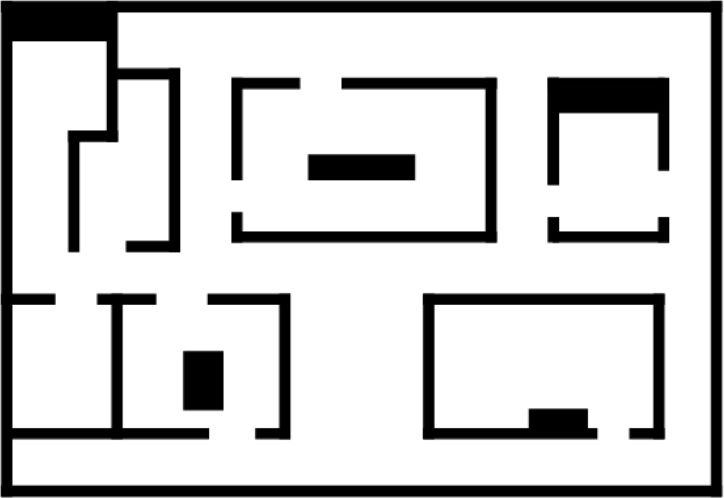
\includegraphics[clip=true, width=0.29\linewidth]{imagenes/tiposDeMapa/metrico.png}\label{fig:ejMapMetrico}}
  \qquad
  \subfloat[Grilla de ocupación]{
\includegraphics[clip=true, width=0.29\linewidth]{imagenes/tiposDeMapa/grillaDeOc.png}\label{fig:ejGrillaOc}}
  \qquad
  \subfloat[Mapa topológico basado en regiones]{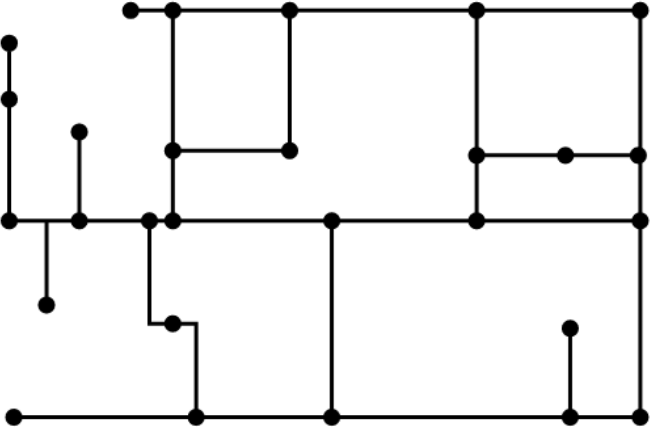
\includegraphics[clip=true, width=0.29\linewidth]{imagenes/tiposDeMapa/topologico.png}\label{fig:ejMapTop}}
  \caption[Tipos de mapas.]{Tipos de mapas. Un mismo entorno representado con distintos tipos de mapas. Extraído de \cite{choset2005principles}.}
\end{figure}

La simplicidad de los mapas topológicos es útil para nosotros los humanos al facilitar la comprensión un entorno y como navegar en él, por lo que es usual ver mapas topológicos de sistemas de transporte (ver figura \ref{fig:metroBsAs}).%, adicionalmente posibilita instrucciones intuitivas como por ejemplo, \say{ir a la habitación A}.

\begin{figure}[H]
  \center
  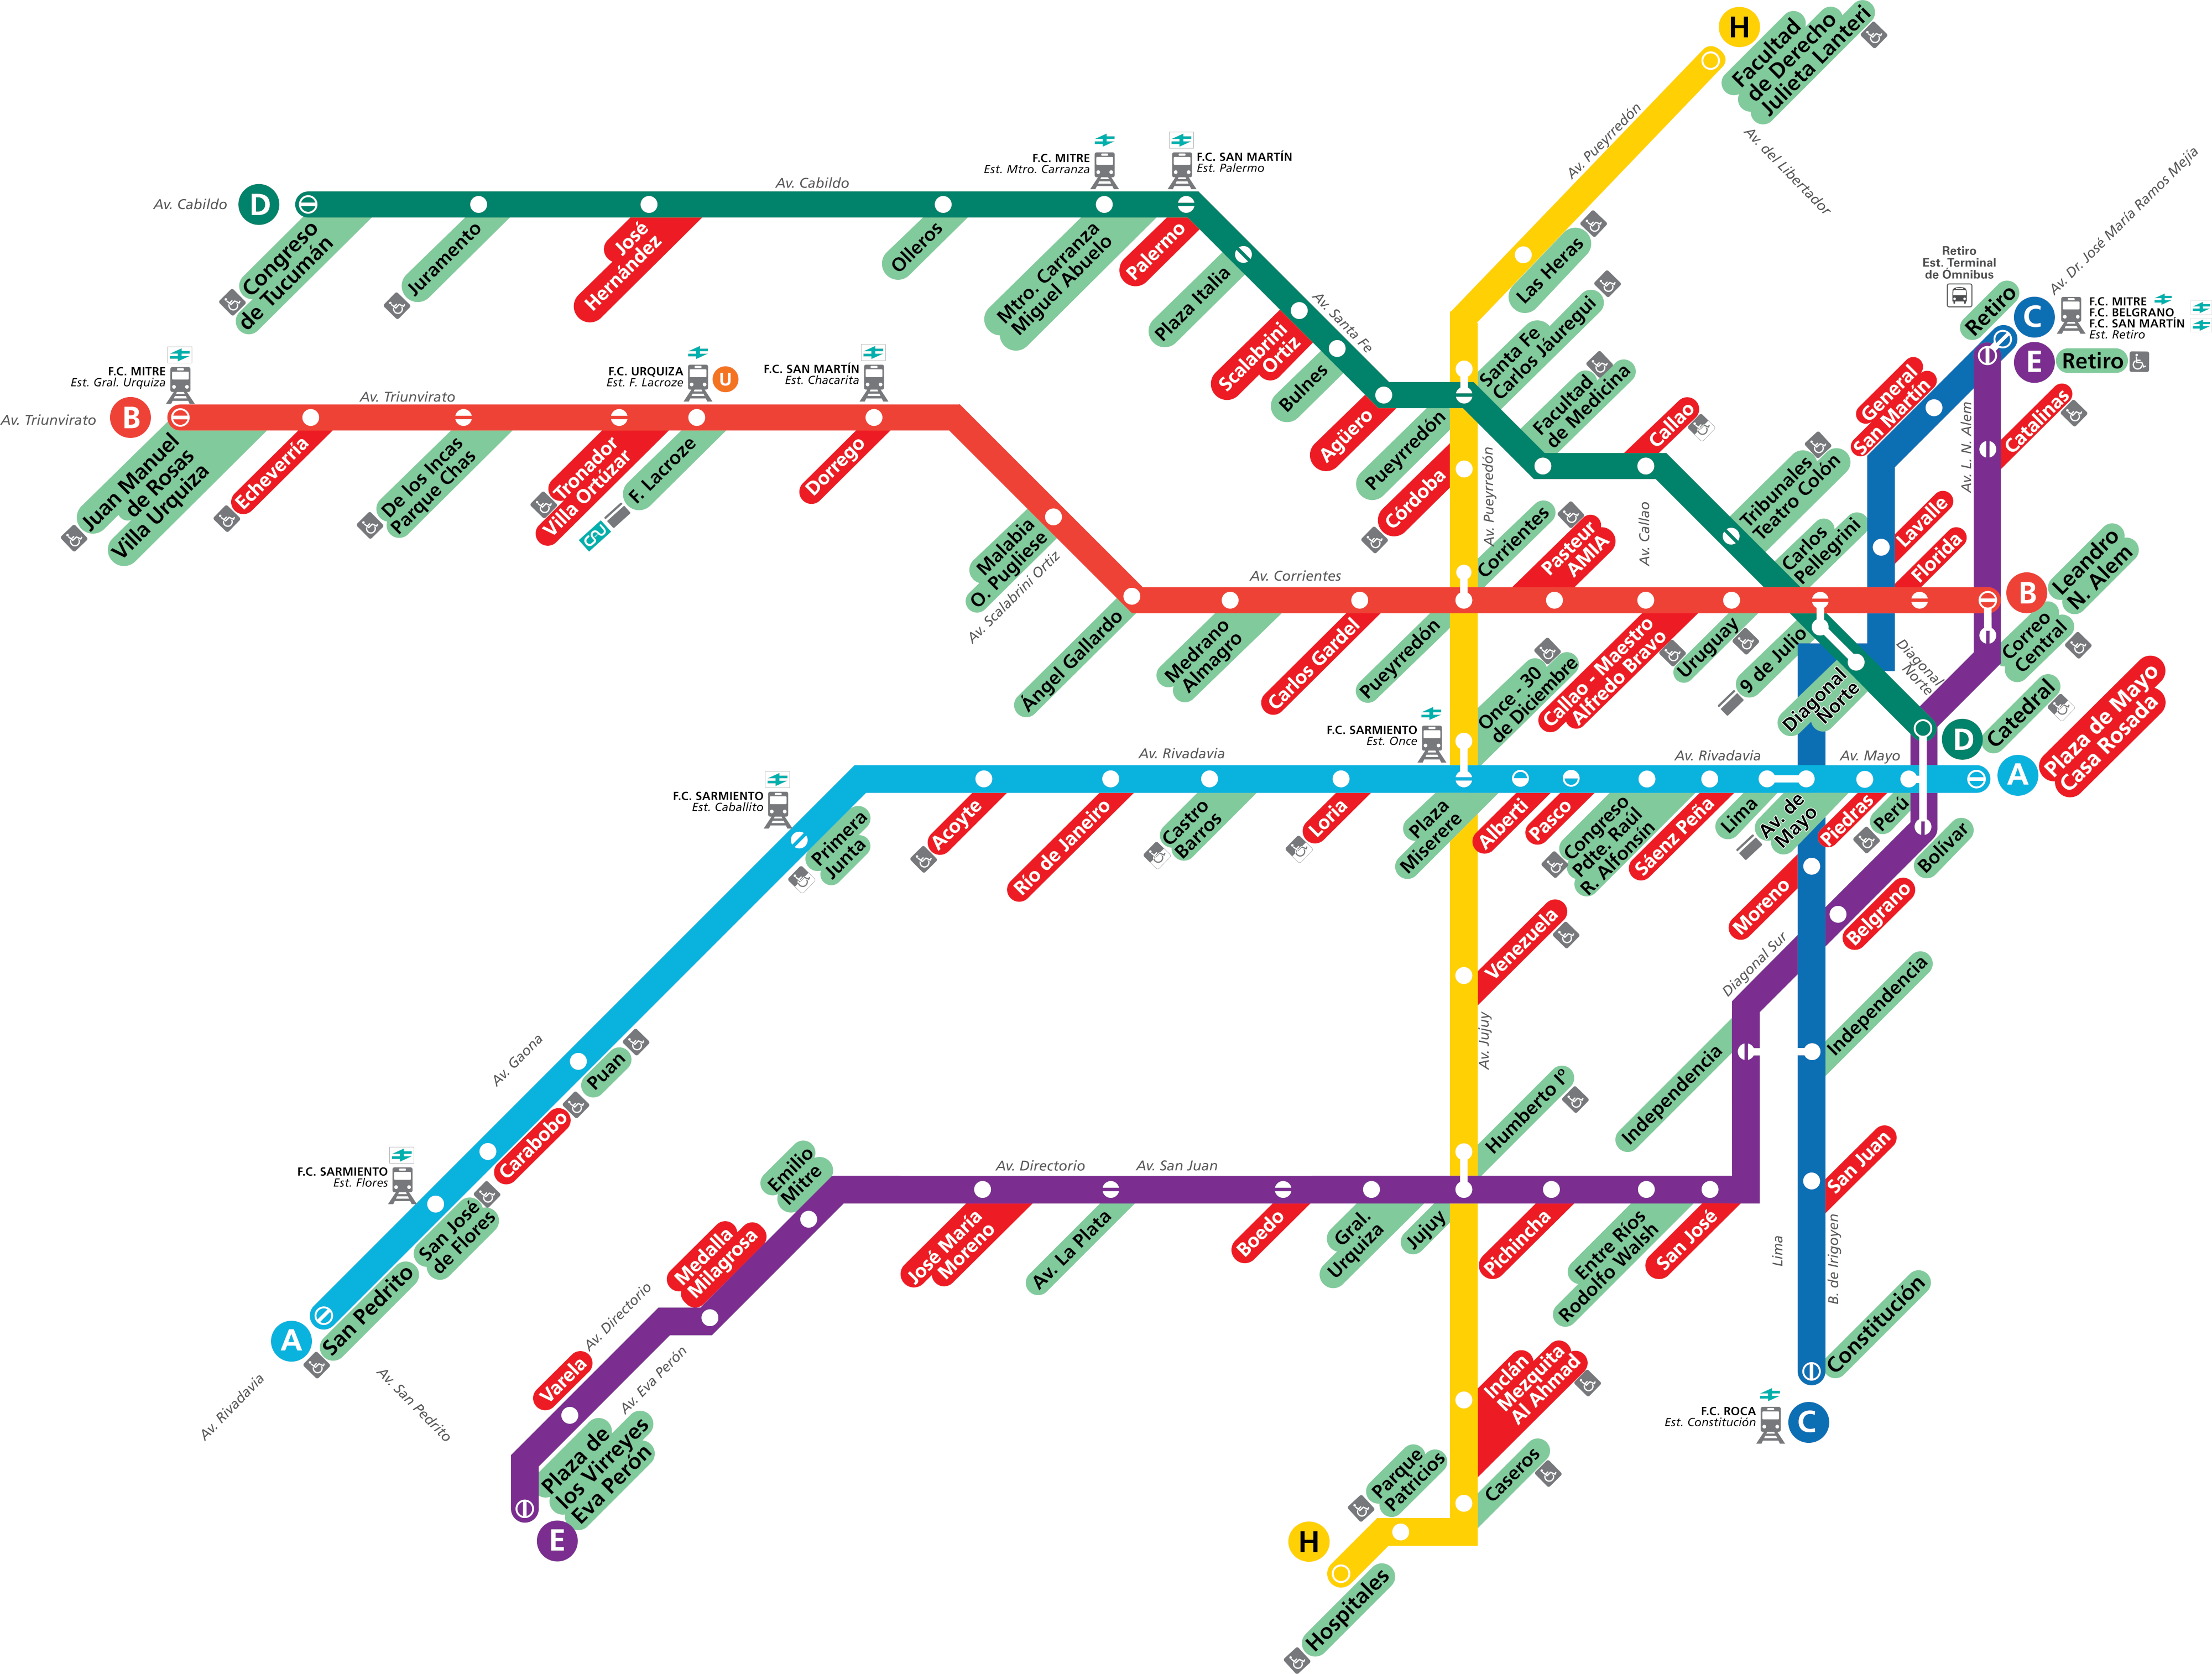
\includegraphics[width=1\linewidth]{imagenes/metroBsAs.png}
  \caption[Mapa del sistema de transporte subterráneo de Buenos Aires, Argentina.]{Mapa del sistema de transporte subterráneo de Buenos Aires, Argentina. Extraído de \cite{metroBsAs}.}\label{fig:metroBsAs}
\end{figure} 

La simplicidad mencionada también tiene ventajas computacionales, ya que para un mismo entorno los mapas topológicos suelen ser ordenes de magnitud más pequeños que los mapas métricos y por lo tanto, más allá de la memoria ahorrada, también se tiene una planificación más eficiente. Sin embargo la falta de detalle en la representación es también una desventaja en tanto hace que los caminos planificados con un mapa topológico suelan ser más largos que los obtenidos en mapas métricos \cite{Thrun1998}.

Dadas las ventajas y desventajas mencionadas existen trabajos \cite{Thrun1998,wurm2008coordinated,Liu2015} que proponen el uso simultáneo de mapas topológicos y métricos para \say{ganar lo mejor de los dos mundos} al tener disponible abstracción y detalle a la vez. Un ejemplo de cómo combinar las ventajas de ambos tipos de mapa es la planificación jerárquica descrita en \cite{Thrun1998} donde se utiliza un mapa topológico y uno métrico de un mismo entorno para generar planes para navegar en el entorno. El mapa topológico es utilizado para generar un plan de navegación topológico que consiste en una secuencia de corredores y habitaciones que se deben atravesar para llegar a un objetivo, plan que aunque es fácil de generar no posee suficiente detalle como para traducirse directamente en acciones que el robot pueda realizar para llegar al objetivo. Por lo tanto se introduce una segunda etapa de planificación que consiste en utilizar la representación métrica del entono para generar planes métricos que permitan al robot moverse entre los segmentos que componen al plan topológico. En este acercamiento se hace un único plan topológico sobre todo el entorno y varios planes métricos sobre porciones reducidas del entorno, lo cual resulta en una reducción del costo computacional en comparación a hacer un único plan métrico sobre el entorno entero.

Los tres trabajos antes mencionados utilizan una misma estrategia para lograr construir un mapa topológico y uno métrico, asegurando que estos son congruentes entre si. La estrategia consiste en construir una grilla de ocupación a partir de los datos obtenidos por los sensores de los robots. Dicha grilla de ocupación es utilizada tanto como mapa métrico, como para generar una estructura intermedia llamada \emph{grafo generalizado de Voronoi}, con el cual es posible detectar los segmentos que constituyen un mapa topológico basado en regiones. Este proceso es una parte fundamental del trabajo desarrollado en este proyecto y se detallará a lo largo de las siguientes secciones.%\todo{durante este proyecto?} 

%\subsection{Mapa métrico basado en polígonos}
%Las grillas de ocupación son los mapas métricos mas utilizadas en el contexto de exploración multirobot, sin embargo, estas grillas no son apropiadas para entornos que son muy grandes o cuyos límites no están bien delimitados desde el comienzo de la exploración. En contraste, las representaciones poligonales no tienen tales limitaciones.

%El artículo \cite{wu2007voronoi} propone utilizar una representación poligonal en la cual el mapa consiste en la union de conjunto de polígonos cerrados de forma y tamaño arbitrario, que pueden estar libres, no explorados u ocupados. 

%Para comprobar y validar la representación propuesta se adapta la estrategia de exploración multirobot presentada en \cite{Solanas2004} (cuya técnica de coordinación fue mencionada en \ref{subsec:coordNoTop}) que originalmente se basa en grillas de ocupación, para que funcione utilizando una representación poligonal.

%De las pruebas realizadas los autores concluyen que una representación poligonal es más compacta, flexible y logra aumentar significativamente la eficiencia.

%\subsubsection{Representación poligonal}
%Inicialmente, todo el mapa estará constituido por un solo polígono desconocido. A partir de lo sensado por cada robot, se incluye nueva información sobre entorno a la representación agregando polígonos libres y ocupados que son substraídos de los polígonos desconocidos a los que pertenecían.

%Los objetivos de exploración se determinan a partir de las aristas entre polígonos desconocidos y polígonos libres denominadas como aristas frontera que son análogas a las celdas frontera de las grillas de ocupación.

%El trabajo propone asignar tareas a partir de la division el entorno desconocido en tantas regiones como robots existan en la flota, para luego asignar a cada robot la tarea de explorar una region diferente. El entorno se divide a partir de un algoritmo que adapta al algoritmo K-Means para funcionar a partir de la representación poligonal propuesta, este algoritmo se explica en la sección\ref{subsubsec:particionamientovoronoi}.  \todo{agregar img}

%%La division del entorno se logra adaptando el algoritmo K-means para funcionar en utilizado para encontrar los centroides correspondientes a las agrupaciones de áreas desconocidas, ya que se asume que estos serán los puntos más provechosos para que los robots exploren.

%Finalmente, la planificación del camino del robot es realizada en el interior de los polígonos libres, cosa que se puede hacer a partir de la aplicación de cualquier algoritmo de descomposición celular, por ejemplo el que se explica en \cite{schachter1978decomposition}.
   
%\subsubsection{Particionamiento basado en polígonos}\label{subsubsec:particionamientovoronoi}
%El diagrama de Voronoi\cite{fortune1987sweepline} de un conjunto de puntos 2D, también conocidos como generadores, $C_{i} , 1 \leq i \leq K$, es una partición de ese espacio en $K$ regiones convexas disjuntas conocidas como células Voronoi. Cada región $V_i$ está definida por los puntos en el espacio que están más cerca de $C_{i}$ que a cualquier otro $C_{j}$, $j\neq i$. \todo{este párrafo bebería escribirse pensando en las definiciones que ya se realizaron. referenciarlas y destacar qué agrega}

%Sea $n$ numero de robots, el resultado deseado es obtener un conjunto de $K=n$ celdas de Voronoi para las cuales, sus centroides (centros de masa) y sus generadores estén a una distancia menos que cierta tolerancia $\varepsilon$. % cerradas que están globalmente delimitadas por el polígono a dividir

%La generación de estas celdas se realiza a partir del algoritmo \ref{alg:particionamientovoronoi} que adapta, utilizado diagramas de Voronoi, al algoritmo K-Means utilizado en la implantación base, que no es compatible con una representación poligonal.

%\begin{algorithm}
%\SetAlgoLined
%    Elegir aleatoriamente $K$ puntos $C_i$, $1 \leq i \leq K$, contenidos en los polígonos correspondientes a las regiones desconocidas actuales en el mapa.\\
%    Calcular el diagrama de Voronoi asociado con el conjunto actual de $C_i$.\\
%    Restringir las celdas del diagrama de Voronoi a los polígonos desconocidos actuales.\\
%    Determinar el centro de masa $M_i$ de cada celda Voronoi restringida.\\
%    \eIf{$C_i - M_i < \varepsilon\ \forall i$}{
%        Saltar al paso 11.\\
%    }{
%        Sustituir cada $C_i$ por su $M_i$ correspondiente.\\ Volver al paso 2.\\
%    }
    
%    Dividir el conjunto de polígonos desconocidos en $K$ regiones disjuntas según las celdas de Voronoi restringidas encontradas.\\
%    \caption{Particionamiento basado en Voronoi}
%    \label{alg:particionamientovoronoi}
    
%\end{algorithm}

%Notar que el algoritmo trabaja con celdas de Voronoi restringidas, estas son las celdas resultantes de un diagrama de Voronoi restringidas a los limites del mapa conocidos por hipótesis.\todo{agregaría una img que ayude a entender cómo funciona}



\subsection{Mapa de carreteras}\label{subsec:mapacarr}
% Un \emph{mapa de carreteras} (del ingles road map) \cite{choset2005principles} es clase particular de mapas topológicos. Que un mapa topológico cumpla con las condiciones necesarias para ser un mapa de carreteras asegura que a partir de este es posible planificar un camino entre dos puntos cualquiera del espacio libre. La idea detrás de esta categoría esta inspirada por como los humanos utilizamos las redes de carreteras. Al planificar un camino entre dos ubicaciónes distantes, por ejemplo dos depatamentos distintos, en lugar de considerar cada camino posible, normalemte planificamos primero un camino hacia una red de carreteras, luego a lo largo de la red de carreteras y, finalmente, desde la red de carreteras hacia el destino. %(ver figura \ref{fig:ejemplovial}). 
Un \emph{mapa de carreteras} (del ingles \emph{roadmap}) \cite{choset2005principles} es una clase particular de mapas topológicos. Que un mapa topológico cumpla con las condiciones necesarias para ser un \emph{roadmap} asegura que a partir de este es posible planificar un camino entre dos puntos cualquiera del espacio libre. La idea detrás de esta categoría esta inspirada por como los humanos utilizamos las redes de carreteras. Al planificar un camino entre dos puntos distantes, por ejemplo ubicados en dos departamentos de Uruguay: Montevideo y Paysandú, en lugar de considerar cada camino posible, normalmente planificamos primero un camino hacia una red de carreteras (Ruta 1), luego a lo largo de la red de carreteras (a través de ruta 1 y ruta 3), para finalmente planificar un camino desde la red de carreteras (Ruta 3) hacia el destino (ver figura \ref{fig:ejemplovial}). 

\begin{figure}[H]
  \center
  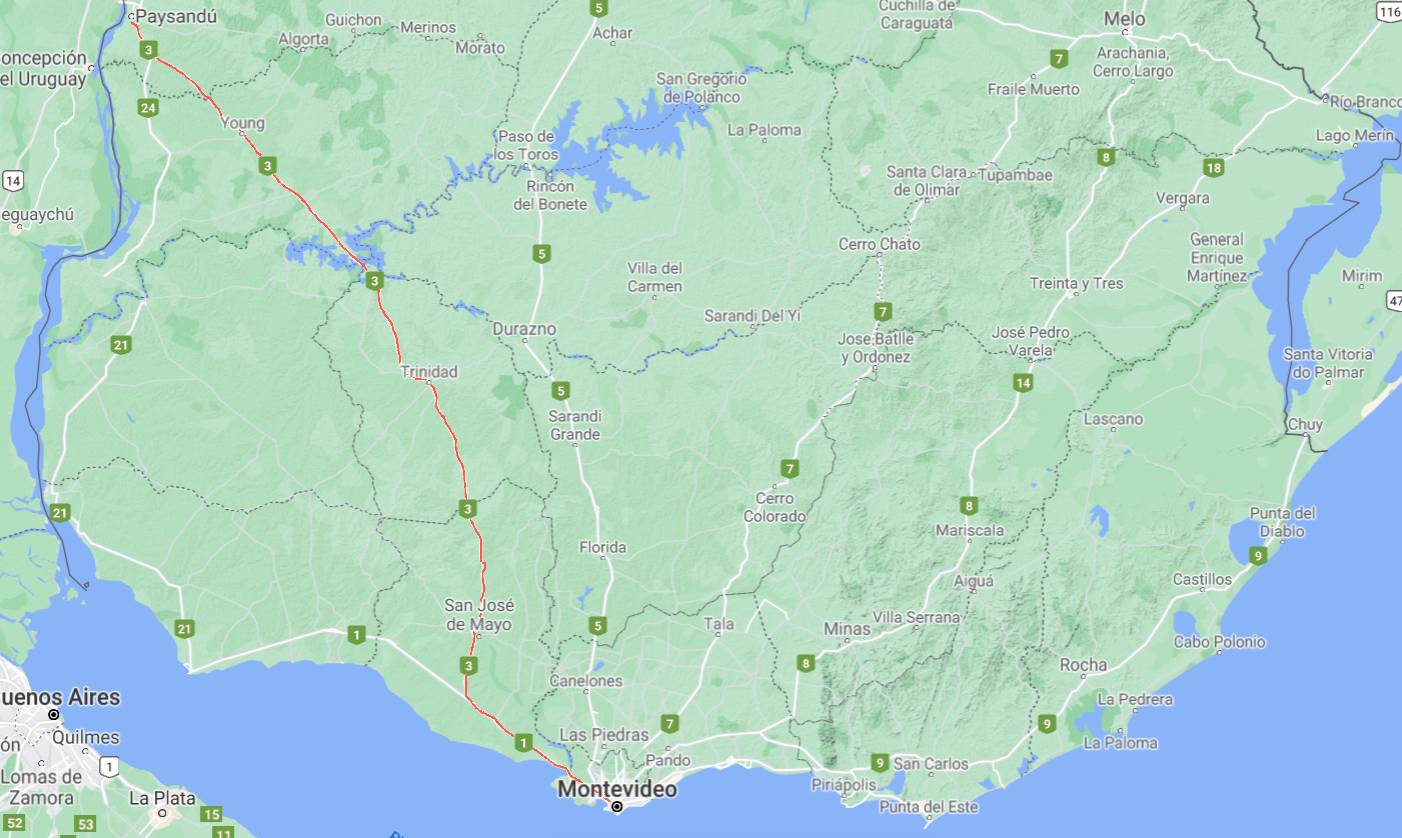
\includegraphics[width=0.9\linewidth]{imagenes/uruguayvialMarcado.png}
  \caption[Red de carreteras de Uruguay.]{Red de carreteras de Uruguay. Con amarillo se resalta un camino entre ubicaciones de Montevideo y Paysandú. Extraído de \cite{googlemaps}.}\label{fig:ejemplovial}
\end{figure} 

Para considerarse un \emph{roadmap}, un mapa topológico debe estar representado
con un grafo $\mli{RM}=(V_{RM},E_{RM})$ en el cual sus vértices $V_{RM}$
corresponden a puntos no ocupados del entorno y sus aristas $E_{RM}$
implican la existencia de al menos un camino disjunto entre los
vértices. Adicionalmente, dicho grafo $\mli{RM}$ debe cumplir con 3
propiedades fundamentales, a partir de las cuales es posible asegurar
que se puede planificar caminos a partir del \emph{roadmap}. Sea $W$ el entorno
y $W_{libre} \subset W$ el espacio libre del entorno, las tres
propiedades son:

\begin{enumerate}
  \item Accesibilidad: Para todo $p_{inicio} \in W_{libre}$ existe un camino a un $p'_{inicio}\in V_{RM}$. % vértice de\todo{sacaría vértice de y en su lugar utilizaría $\in V$, si lo definimos antes. ídem en lo sucesivo.} $\mli{RM}$.
  \item Conectividad: Existe un camino entre cualquier par $p'_{inicio},\ p'_{fin} \in V_{RM}$.
  \item Capacidad de salida: Para todo $p'_{fin} \in V_{RM}$ existe un camino a un $p_{fin} \in W_{libre}$.
\end{enumerate}

Estas propiedades aseguran la navegación, porque que dados dos puntos $p_{inicio},\ p_{fin}\in W_{libre}$ es posible construir un camino entre ellos. Primero por \emph{accesibilidad} se tiene un camino entre $p_{inicio}$ y un $p'_{inicio}\in \mli{RM}$, luego por \emph{capacidad de salida} se asegura la existencia de un  $p'_{fin}\in \mli{RM}$ desde el cual hay un camino a $p_{fin}$ y finalmente por \emph{conectividad} se sabe que existe un camino entre $p'_{inicio}$ y $p'_{fin}$. Entonces uniendo los caminos $p_{inicio} - p'_{inicio}$ (por accesibilidad), $p'_{inicio} - p'_{fin}$ (por conectividad) y $p'_{fin} - p_{fin}$(por capacidad de salida) se tiene un camino que conecta dos puntos genéricos del espacio libre $p_{inicio}$ y $p_{fin}$.

% \cite{choset2005principles}, \cite{Thrun1998}, \cite{Liu2015}.
\subsection{Diagrama de Voronoi}\label{sec:VD}
Dado un espacio euclídeo $W \subseteq R^2$, y $G \subset W$ un conjunto de puntos llamados \emph{generadores}. Sea $p\in W$, la función $d_p : W \rightarrow R$ qué computa la distancia desde $p$ a otro punto en $W$. 

% Una \emph{region de Voronoi} $R_i\subset W$ es el conjunto de puntos mas cercanos a un generador $s_i\in G$ particular: 
% \begin{equation}
%   R_i = \{p \in W : d_p(s_i) \leq d_p(s_j), s_i,s_j\in G,s_j \neq s_i\}\label{eq:regV}
% \end{equation}
Los \emph{puntos bases} de $p$, $BP_p \subseteq G$ son el conjunto de generadores más cercanos a un punto $p \in W$ :
\begin{equation}
  \mli{BP}_p =\{s_i \in G : d_p(s_i) \leq d_p(s_j), \forall s_j\in G,s_j \neq s_i\}\label{eq:bases}
\end{equation}

Un \emph{diagrama de Voronoi} $\mli{VD}\subset W$ se define como todos los puntos con dos o más generadores a una misma mínima distancia, o lo que es equivalente, que tienen dos o más puntos base: 
\begin{equation}
  \mli{VD} = \{p \in W : |\mli{BP}_p| \geq 2\}\label{eq:VD}
\end{equation}

% Notar que las fronteras de las regiones de Voronoi forman parte del diagrama de Voronoi por lo que es posible decir que un diagrama de Voronoi secciona el espacio en regiones de Voronoi. 
% Una propiedad de los diagramas de Voronoi es que los puntos que pertenecen a el serán máximos locales no estrictos de distancia a los generadores. Esta propiedad es útil en el contexto de la robótica porque permite asegurar que los caminos en un diagrama de Voronoi generado con el conjunto de obstáculos como generadores son seguros en tanto mantienen la mayor distancia posible a los obstáculos.

En la figura \ref{fig:ejemploVoronoi} se muestra un ejemplo de un diagrama de Voronoi, con $G=\{A_i | 1\leq i \leq 10\}$ como generadores.
\begin{figure}[H]
  \center
  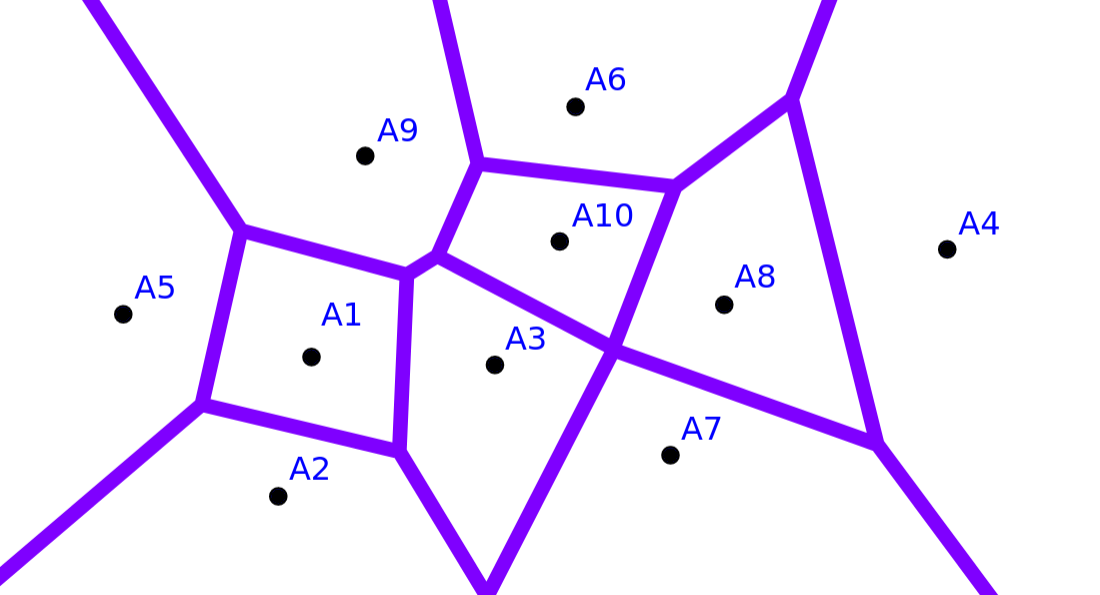
\includegraphics[width=5.5cm]{imagenes/VD.png}
  \caption[Diagrama de Voronoi.]{Diagrama de Voronoi. Con negro se indican los generadores, mientras que con violeta se indican los puntos pertenecientes al diagrama de Voronoi. Generado con \cite{voronoigeo}.}\label{fig:ejemploVoronoi}
\end{figure} 

Una propiedad de los diagramas de Voronoi es que los caminos sobre este tipo de diagramas mantienen a lo largo de ellos la mayor distancia posible al generador más cercano.
Esta propiedad es útil en el contexto de la robótica porque dado un diagrama de Voronoi generado con el conjunto de obstáculos como generadores, los caminos sobre este se consideran caminos de máxima seguridad en tanto mantienen al robot lo más alejado posible de los obstáculos durante el recorrido.

% Una propiedad de los diagramas de Voronoi  es que los caminos sobre este tipo de diagramas aseguran mantener la mayor distancia posible a los generadores. Esta propiedad es util en el contexto de la robotica porque permite asegurar por lo tanto en un diagrama de Voronoi generado con el conjunto de obstáculos como generadores se puede decir que los caminos sobre este serán seguros en tanto mantienen la mayor distancia posible a los obstáculos.

 % \cite{choset2005principles}, \cite{latombe1991}, \cite{wurm2008coordinated}
\subsection{Diagrama generalizado de Voronoi}\label{subsec:GVD}
Recordando que los generadores en un diagrama de Voronoi son puntos, se tiene un problema al querer utilizar obstáculos como generadores. El problema radica en que normalmente los obstáculos ocupan un área y por lo tanto no pueden representarse como puntos en el espacio, para solucionar esto se generaliza la definición de diagrama de Voronoi para poder definirlo a partir de generadores de mayor orden, como lo son líneas o polígonos. A esta generalización se la denomina como \emph{diagrama generalizado de Voronoi} $\mli{GVD}\subset W$ , y los generadores de mayor orden o generadores generalizados son representados como conjuntos de puntos del espacio de trabajo, siendo $\mli{GG}\subset P(W)$ el conjunto de todos los generadores generalizados.

% Las nuevas definiciones generalizadas son en su mayoría análogas a las originales, siendo el principal cambio la substitución de la función de distancia $d_p$ por una función de distancia generalizada $\mli{gd}_p : 2^{W} \rightarrow R$ que considera las formas de los generadores generalizados. La función $\mli{gd}_p$ se define a partir de $d_p$ como se muestra en la ecuación \ref{eq:dg}.

Las definiciones relacionadas a los GVD consisten en generalizaciones de
las planteadas para los VD en la sección \ref{sec:VD} pensadas para considerar
generadores generalizados en lugar de generadores puntuales. 
En primer lugar se define la llamada función de distancia generalizada
$\mli{gd}_p : P(W) \rightarrow R$ que permite obtener la distancia entre
$p$ y un generador generalizado $s_i$, definida a partir de la distancia
euclídea $d_p$ como se muestra en \eqref{eq:dg}.
\begin{equation}
  \mli{gd}_p(s_i) = \min_{p'\in s_i}\{d_p(p')\} \label{eq:dg}
\end{equation}
A partir de la distancia generalizada se definen los generadores base
generalizados $\mli{GBG}_p\subseteq GG$ como los generadores más
cercanos a un punto $p$ \eqref{eq:GBG}. Notar que estos son la
generalización de los puntos base del VD.
\begin{equation}
  \mli{GBG}_p = \{s_i \in \mli{GG}: \mli{dg}_p(s_i) \leq \mli{dg}_p(s_j), \forall s_j\in \mli{GG}, s_j \neq s_i\}\label{eq:GBG}
\end{equation}
Finalmente la definición $\mli{GVD}$ es análoga a su contra parte no
generalizada y se define según se muestra en \eqref{eq:GVD}. 
%, a partir de los cuales se puede definir los puntos base generalizados $\mli{GBP}_p$ de un punto $p$ como los puntos pertenecientes a los generadores de $\mli{GBG}_p$ que son más cercanos a $p$ \eqref{eq:GBP}. 

%\todo{de acuerdo, GBG no aporta, alcanza con GG}
% \todo[inline]{En la def de GBP si en la U se usa GG entonces por cada conjunto de puntos que compone obstaculo $s_i$ en $GG$ se tiene al menos un punto base (argmin se aplica a cada obstaculo individualmente) entoces si hay dos obstaculos ya se tiene que todo punto pertenece al GVD, restingir la U a solo los obstaculos a mínima distancia soluciona esto. Otra solucion es redefinir GBP para decir algo como: los puntos a mínima distancia de cualquier obstaculo, pero me parece mas claro usar GBG y la U de argmin. Cambie el principio del parrafo para indicar que es util mas que necesario, igual lo hablamos a ver que es mejor de las alternativas| para mi GBG no es necesario, con GG alcanza. sacaría}La definición $\mli{GVD}$ es análoga a su contra parte no generalizada y se define según se muestra en \eqref{eq:GVD}. 
% Las regiones generalizadas de Voronoi $\mli{GR}_i$ y el diagrama generalizado de Voronoi $\mli{GVD}$ son las definiciones mas similares a sus contra partes no generalizadas y se definen según se muestra en \eqref{eq:GR} y \eqref{eq:GVD} respectivamente. 

% Notar que la definición de puntos base generalizados tiene una modificación adicional al cambio en la función de distancia, esta es que en lugar de devolver los generadores generalizados mas cercanos $\mli{GBG}_p$\ref{eq:GBS}, solo devuelve los puntos mas cercanos de estos.


% \begin{equation}
%   \mli{GBP}_p =\{p' \in W : d_p(p') \leq d_p(p''), p' \in s_i, p'' \in s_j, s_i,s_j \in \mli{GG},p' \neq p''\}
% \end{equation}
% \begin{equation}
%   \mli{GBP}_p =\bigcup_{s_i \in \mli{GBG}_p} \argmin_{p'\in s_i}\{d_p(p')\}\label{eq:GBP}
% \end{equation}
\begin{equation}
  \mli{GVD}  = \{p \in W : |GBG_p| \geq 2\}\label{eq:GVD}
\end{equation}
% \begin{equation}
%   \mli{GR}_i = \{p \in W : \mli{dg}_p(s_i) \leq \mli{dg}_p(s_j), s_i,s_j\in \mli{GG},s_j \neq s_i\}\label{eq:GR}
% \end{equation}

Algo a destacar sobre los GVD es que la distribución de los puntos sobre los
generadores generalizados no es un tema trivial. Volviendo al caso en el se
desea utilizar los obstáculos como generadores, el problema se traduce a la
distribución los puntos obstaculizados en generadores generalizados. Una
distribución razonable es la resultante de utilizar los conjuntos conexos de
puntos obstaculizados como generadores. Esta decisión lleva a resultados que
pueden no ser deseados, por ejemplo dentro de una habitación vacía no va a
existir ningún punto perteneciente al GVD (figura \ref{fig:distGenConex}). Esto
se debe a que las cuatro paredes conforman un único obstáculo y por lo tanto
para cualquier punto $p$ dentro de la habitación se tiene que $|GBG_p| = 1$.
El resultado se repite para cualquier generador cóncavo que no contenga otros
generadores en su interior, como es el caso de las habitaciones de una sola
entrada, y de los corredores sin salida. De esta última observación se deriva
el criterio presentado en \cite{choset2005principles} que consiste en utilizar
como generadores a conjuntos que ademas de ser conexos sean convexos, evitando
así generadores cóncavos. En la figura \ref{fig:distGenConvex} se muestra un
ejemplo de distribución de puntos obstaculizados en generadores conexos y
convexos junto al GVD generado en el interior de la habitación. 
% Otra técnica para este tipo de inconvenientes
% es la usada en \cite{Lau2010} que se reduce a considerar como generadores a los
% conjuntos unitarios integrados por cada punto obstaculizado, con esto se
% obtienen resultados similares a los obtenidos usando conjuntos conexos y
% convexos (iguales para el caso de la figura \ref{fig:distGenConvex}).

\begin{figure}[H]
  \centering
  \subfloat[Generadores conexos]{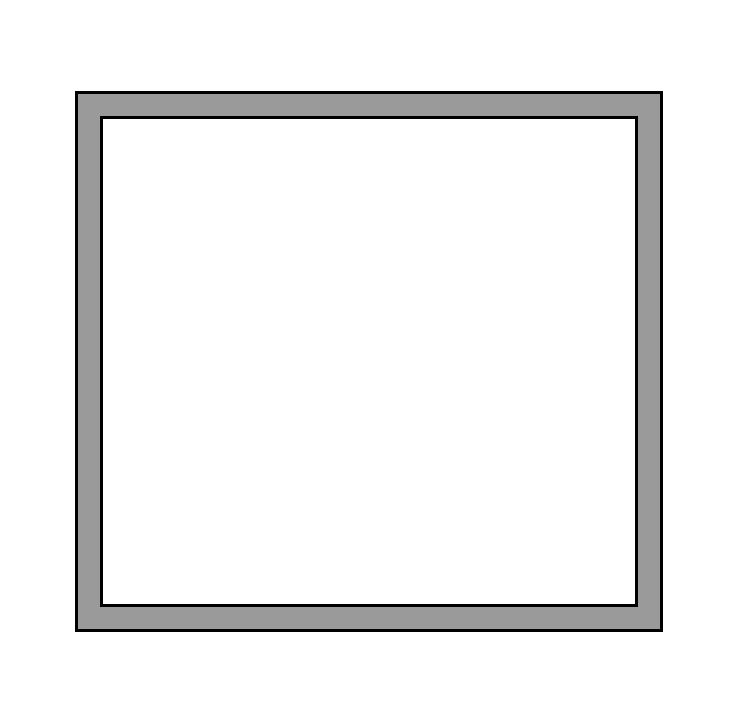
\includegraphics[clip=true, width=0.45\linewidth]{imagenes/GVDG/conex.png}\label{fig:distGenConex}}
  \qquad
  \subfloat[Generadores conexos y convexos.]{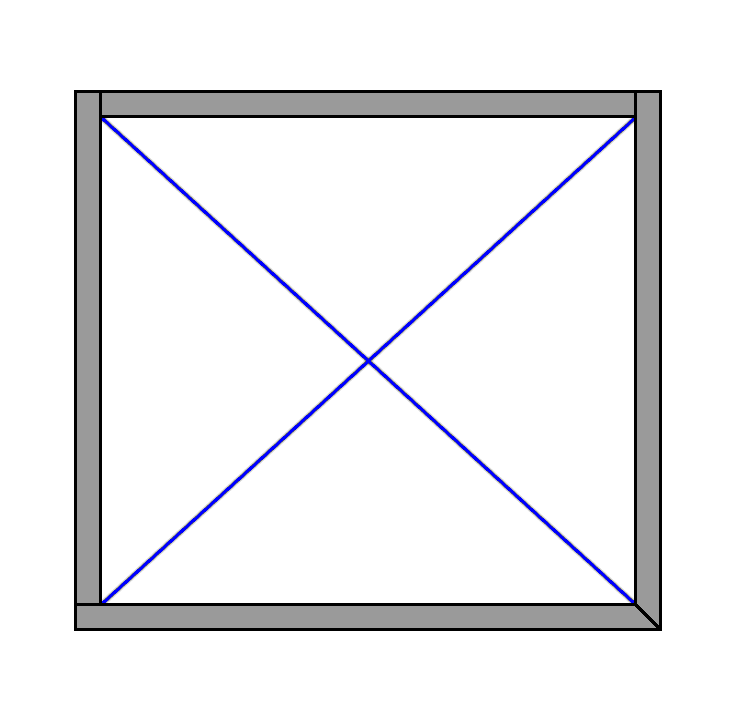
\includegraphics[clip=true, width=0.45\linewidth]{imagenes/GVDG/convex.png}\label{fig:distGenConvex}}
  \caption[Distribución de generadores.]{Distribución de generadores. Los generadores se indican con polígonos de interior gris delimitados con aristas negras mientras que el GVD se indica con azul.}\label{fig:distriGen}
\end{figure}

En la figura \ref{fig:ejemploGVD} se muestra un ejemplo de un GVD que es posible obtener usando generadores conexos y convexos.
%y convexos o generadores unitarios.  

\begin{figure}[H]
  \centering
  % \subfloat[GVD]{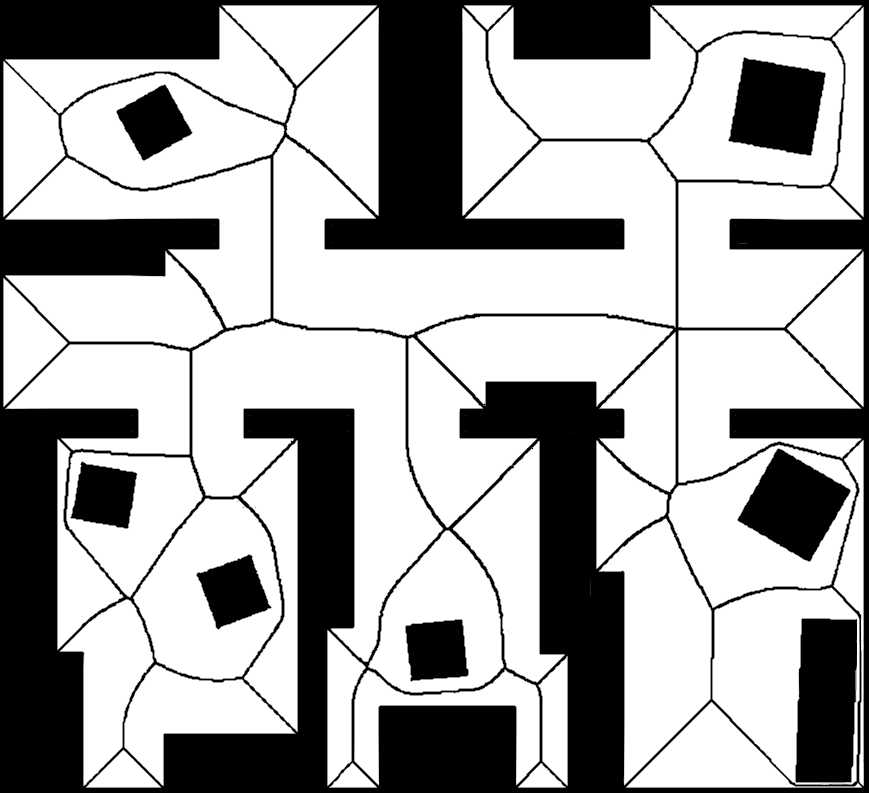
\includegraphics[clip=true, width=0.45\linewidth]{imagenes/GVD2.png}\label{fig:ejemploGVD}}
  % \qquad
  % \subfloat[Grafo asociado al GVD.]{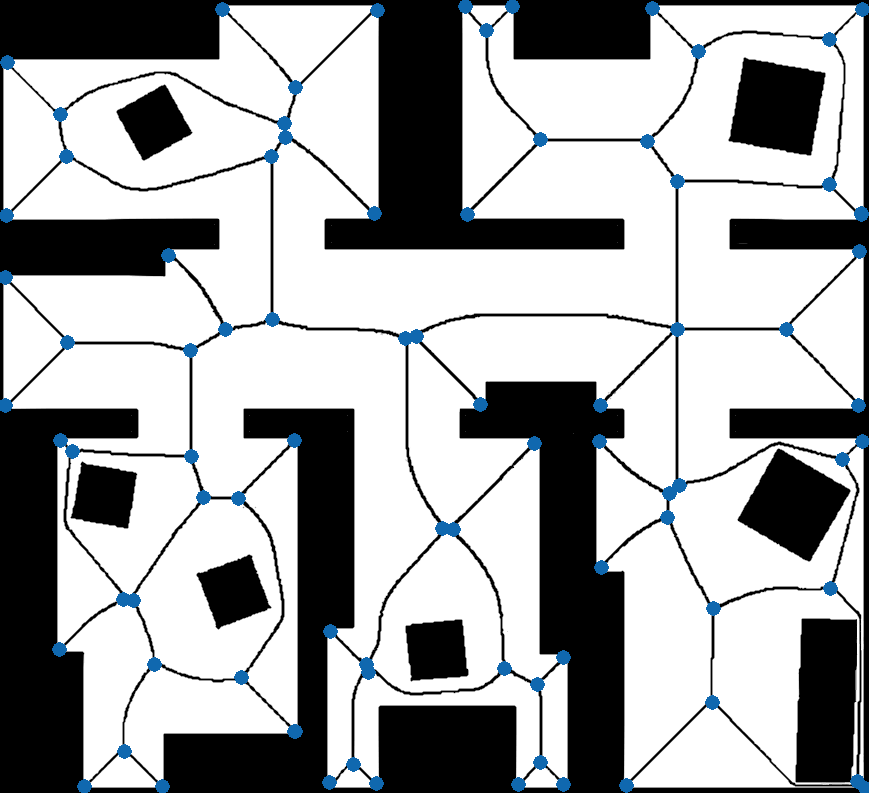
\includegraphics[clip=true, width=0.45\linewidth]{imagenes/GVDGraph.png}\label{fig:ejemploGVDgrafo}}
  % \subfloat[GVD]{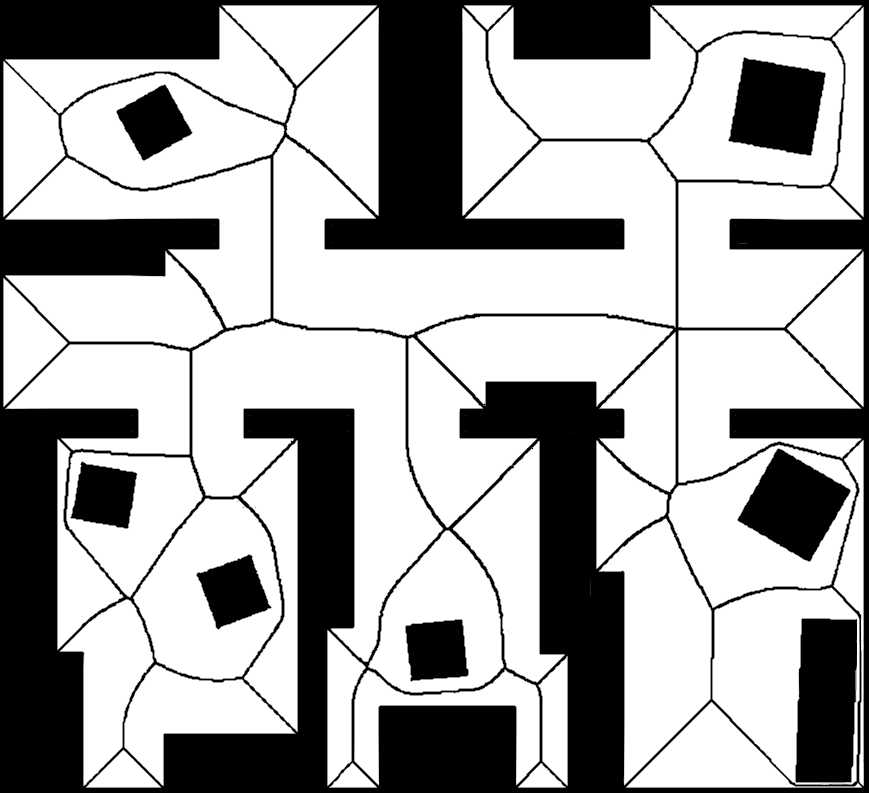
\includegraphics[clip=true, width=0.45\linewidth]{imagenes/GVD2.png}\label{fig:ejemploGVD}}
  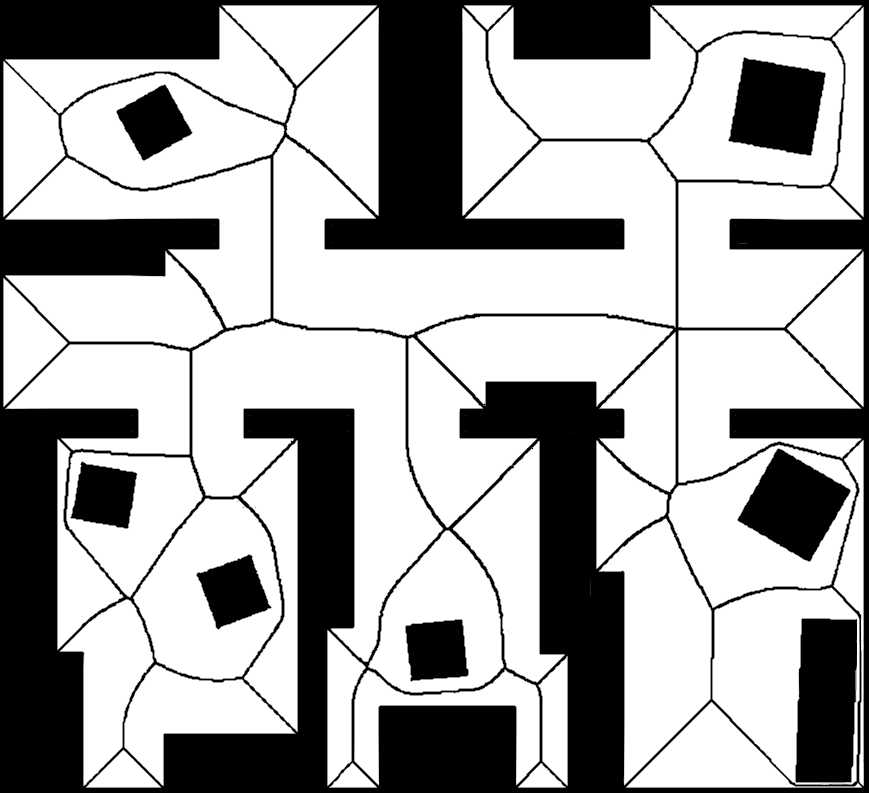
\includegraphics[width=0.45\linewidth]{imagenes/GVD2.png}
  \caption[Diagrama generalizado de Voronoi.]{Diagrama generalizado de Voronoi. El espacio libre se marca con blanco, las líneas negras identifican al GVD y los polígonos negros representan obstáculos. Extraído de \cite{Wallgrun2005}}\label{fig:ejemploGVD}
\end{figure}


% vértices son los puntos pertenecientes al GVD, y las aristas están entre los vértices adyacentes en el espacio. Por otro lado otra forma mas compacta es que los 
% Para referirse a la segunda forma, mas compacta, de representar el GVD con un grafo se utilizara el termino grafo colapsado, y para la primera forma, el termino utilizado es grafo descolapsado. 
% Los GVD suelen ser representados con un grafo en el cual los vértices son los puntos $p$ pertenecientes al GVD que son adyacentes a obstáculos o que cumplen con $|\mli{GBP}_p|\geq 3$, mientras que las aristas\todo{muy entreverado. en un grafo las aristas conectan vértices. de hecho, ahora que lo observo, lo de la fig.1.5b no es un grafo. las aristas no son curvas ya que no modelan dicha información.} se encuentran entre los vértices que se encuentran conectados por caminos disjuntos formados por puntos pertenecientes al GVD. En la figura \ref{fig:ejemploGVDgrafo} se muestra el grafo asociado al GVD de la figura \ref{fig:ejemploGVD}, donde los círculos rojos son los vértices del grafo y las líneas negras las aristas. %(aunque no son visibles existen aristas entre los vértices correspondientes a puntos que son tan cercanos que se solapan)\todo{no creo que este paréntesis aporte}.

En \cite{choset2005principles} se demuestra que los GVD que utilizan los
conjuntos conexos y convexos de puntos obstaculizados como generadores cumplen
con las 3 propiedades necesarias para ser \emph{roadmaps} (sección
\ref{subsec:mapacarr}), lo cual justifica su uso para la navegación. Esto junto
a la capacidad de generar caminos seguros ya mencionada y a otras
características como su utilidad para la coordinación y para generar mapas
topológicos basados en regiones que se tratarán más adelante, hacen que los GVD
que utilizan obstáculos como generadores, sean estructuras de gran útilidad en
el contexto de la navegación robótica. De ahora en adelante al hablar de GVD se
hace referencia a GVD generado considerando a los conjuntos conexos y convexos
de puntos obstaculizados como generadores.

% Otra definición alternativa de GVD se muestra en \eqref{eq:GVDalt}, esta definición es mas restrictiva que la anterior en tanto no permite que un punto pertenezca si tiene mas de dos puntos bases pero estos pertenecen a un mismo generador. Esta definición trae problemas ya que distintas formas de separar a los obstáculos en generadores puede causar distintos GVD. Por ejemplo si se considera u generador como un conjunto conexo de puntos ocupados se tiene que en el interior de las habitaciones con una entrada no se generara GVD, ya que sus paredes por estar conectadas serán un solo generador, y por lo tanto los puntos $p$ interiores a la habitación aunque pueden cumplir con $|GBP_p| \geq 2$ no cumplirán con $|GBS_p| \geq 2$.
% \begin{equation}
%   \mli{GVD}  = \{p \in W : |GBS_p| \geq 2\}\label{eq:GVDalt}
% \end{equation}

%%%%%%%%%%%%%%%%%%%%%%%%%%%%%%%%

% Esto  necesita asumir que los obstáculos son convexos para poder entenderse porque por ejemplo si se considera las 4 paredes de una habitación como un único obstáculo eso seria un único generador generalizado y no formaría un GVD.

% En la def que use también es necesario  porque podrían darse pequeñas imperfecciones en un espacio continuo que generen que lo que a escala macroscópica es una pared a escala microscópica sean tenga pequeñas hendiduras circulares que causen puntos pertenecientes al GVD en lugares no deseados. Esto se evita considerando obstáculos convexos. 

% La ventaja de la forma que use es que no requiere entrar en los asuntos de obstáculos convexos para un entendimiento superficial, mientras que en la otra si.

% \end{figure} 
\subsection{Construcción de un GVD}\label{subsec:constGVD}
% Existen dos tipos principales de métodos para la construcción de un GVD\cite{choset2005principles} los basados en sensores y los basados en grillas\todo{colocaría una cita al lado de cada una. también, discutiría un poco sus diferencias, bondades y debilidades. como para fundamentar un poco la elección.}. En el contexto del trabajo desarrollado serán relevantes los métodos de construcción basados en grillas.

Una idea intuitiva para construir un GVD en un espacio representado con una grilla es la de definir un criterio que determine la pertenencia de una celda al GVD y luego aplicarlo celda a celda. Un criterio posible consiste en que una celda debe pertenecer al GVD si tiene dos o más celdas ocupadas a una misma distancia, siendo la distancia entre celdas la distancia entre sus centros. Sin embargo, esta técnica genera resultados erróneos al no considerar los efectos causados por la discretización. Por ejemplo, en corredores cuya discretización resulta en una cantidad par de celdas entre sus paredes, según este método ninguna celda debería pertenecer al GVD dado que ninguna  tendría una misma distancia a dos celdas ocupadas (paredes del corredor). Esto se considera incorrecto porque el GVD construido en un espacio discretizado debe corresponder al GVD que se construiría en el mismo espacio si fuera continuo y  en el caso continuo los puntos del centro de un corredor siempre pertenecen al GVD. %El método de \cite{wurm2008coordinated} soluciona este tipo de problemas porque la esqueletización asegura la generación de puntos pertenecientes al GVD en las 

En \cite{wurm2008coordinated} se propone un método que logra construir un GVD evitando los problemas de discretización mencionados. El método comienza aplicando una transformación de distancia Euclidiana \cite{meijster2002general} a una mapa métrico representado con una grilla donde cada celda esta ocupada o libre, resultando en un mapa que contiene para cada celda la distancia al obstáculo más cercano, este tipo de mapa se denomina \emph{mapa de distancia} a los obstáculos. Finalmente GVD se obtiene aplicando un algoritmo de esqueletización \cite{zhang1984fast} al mapa de distancia construido. Un ejemplo de este proceso se puede ver en la figura \ref{fig:wurmGVD}. En esta propuesta es clave el uso del algoritmo de esqueletización, que retrae el mapa de distancias a un esqueleto discreto que se aproxima al GVD que se generaría en el espacio continuo.   

% que consiste en erosionar las celdas mas cercanas a los obstáculos hasta llegar a las celdas mas distantes a estos siendo estas últimas las celdas que se asignan al GVD construido. Un ejemplo de este proceso se puede ver en la figur
\begin{figure}[H]
  \centering
  \subfloat[Mapa original]{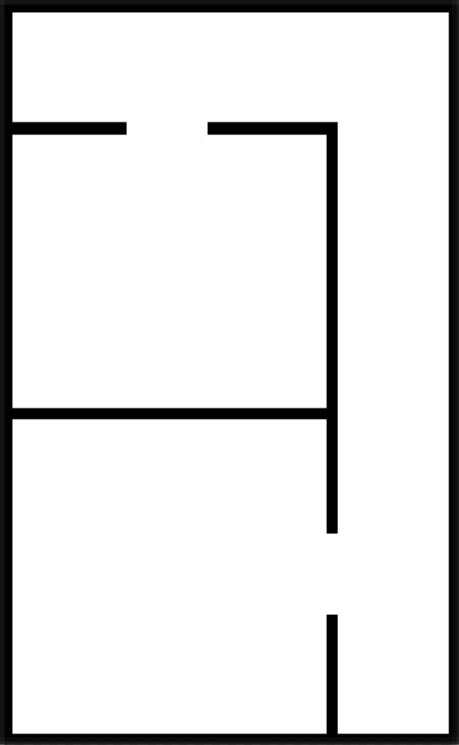
\includegraphics[clip=true, width=0.29\linewidth]{imagenes/wurmSeg/a.png}\label{fig:ejWurmA}}
  \qquad
  \subfloat[Mapa original y mapa de distancia (oscuridad proporcional a la distancia al obstáculo más cercano)]{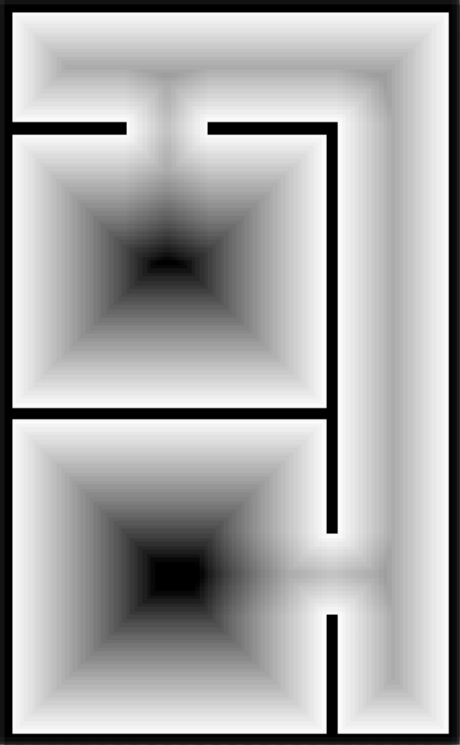
\includegraphics[clip=true, width=0.29\linewidth]{imagenes/wurmSeg/b.png}\label{fig:ejWurmB}}
  \qquad
  \subfloat[Mapa original y GVD (resultante de la esqueletización)]{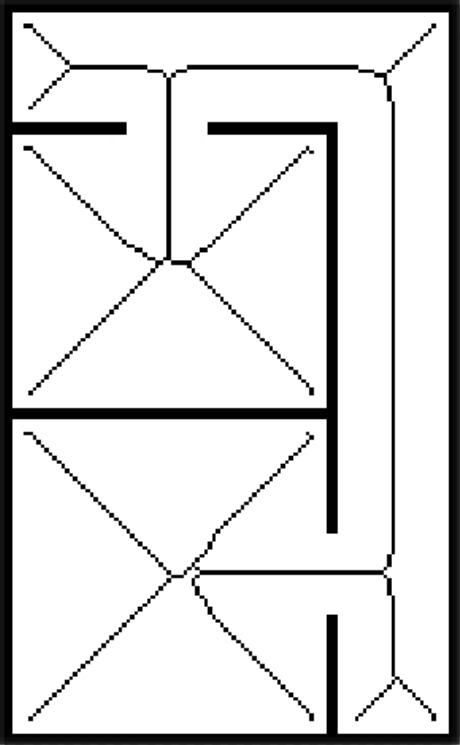
\includegraphics[clip=true, width=0.29\linewidth]{imagenes/wurmSeg/c.png}\label{fig:ejWurmC}}
  \caption[Método de construcción de un GVD.]{Método de construcción de un GVD. Extraído de \cite{wurm2008coordinated}.}\label{fig:wurmGVD}
\end{figure}

Otro método es el presentado en \cite{choset2005principles} llamado
\emph{brushfire} que permite construir un GVD mientras se determina un mapa de
distancia a los obstáculos.
%, asociado a una grilla donde cada celda tiene asociado un estado libre u ocupado.
Este algoritmo se puede ver como una variante con multiples fuentes y sin
destino del conocido algoritmo de Dijkstra, en el que las fuentes son los
obstáculos y la distancia calculada es la mínima distancia hacia un obstáculo.
Se comienza inicializando las distancias de las celdas libres con $\infty$ y
las ocupadas con $0$.  Adicionalmente, las celdas ocupadas se insertan en una
cola de prioridad que prioriza las celdas de menor distancia. Luego hasta que
las cola de prioridad este vacía se remueve la celda más prioritaria $c$ y para
cada celda $c'$ adyacente a $c$ se computa una distancia tentativa $dt_{c'}$
según \eqref{ec:dtBrushFire} que remplaza la distancia actual $d_{c'}$ de la
celda $c'$ si $dt_{c'}<d_{c'}$. De reemplazarse $d_{c'}$ se inserta a $c'$ en
la cola de prioridad. 

\begin{equation}\label{ec:dtBrushFire}
  dt_{c'} = d_c+||c'-c||_2
\end{equation}

Una vez que la cola de prioridad queda vacía, el valor de distancia de las celdas converge al valor de la mínima distancia hacia un obstáculo. 

El nombre de este algoritmo proviene de como este determina las distancias comenzando desde cada obstáculo y extendiéndose desde las celdas más cercanas a las más lejanas asemejándose a un incendio de maleza (traducido al ingles como brushfire). Adicionalmente el algoritmo también puede interpretarse como ondas que parten desde cada obstáculo, y a medida de que avanzan le asignan la distancia recorrida a las celdas que atraviesan. Un ejemplo de ejecución se muestra en la figura \ref{fig:wavesBrush}.  
% a cada celda por la que pasan mientras avanzan

\begin{figure}[H]
  \center
  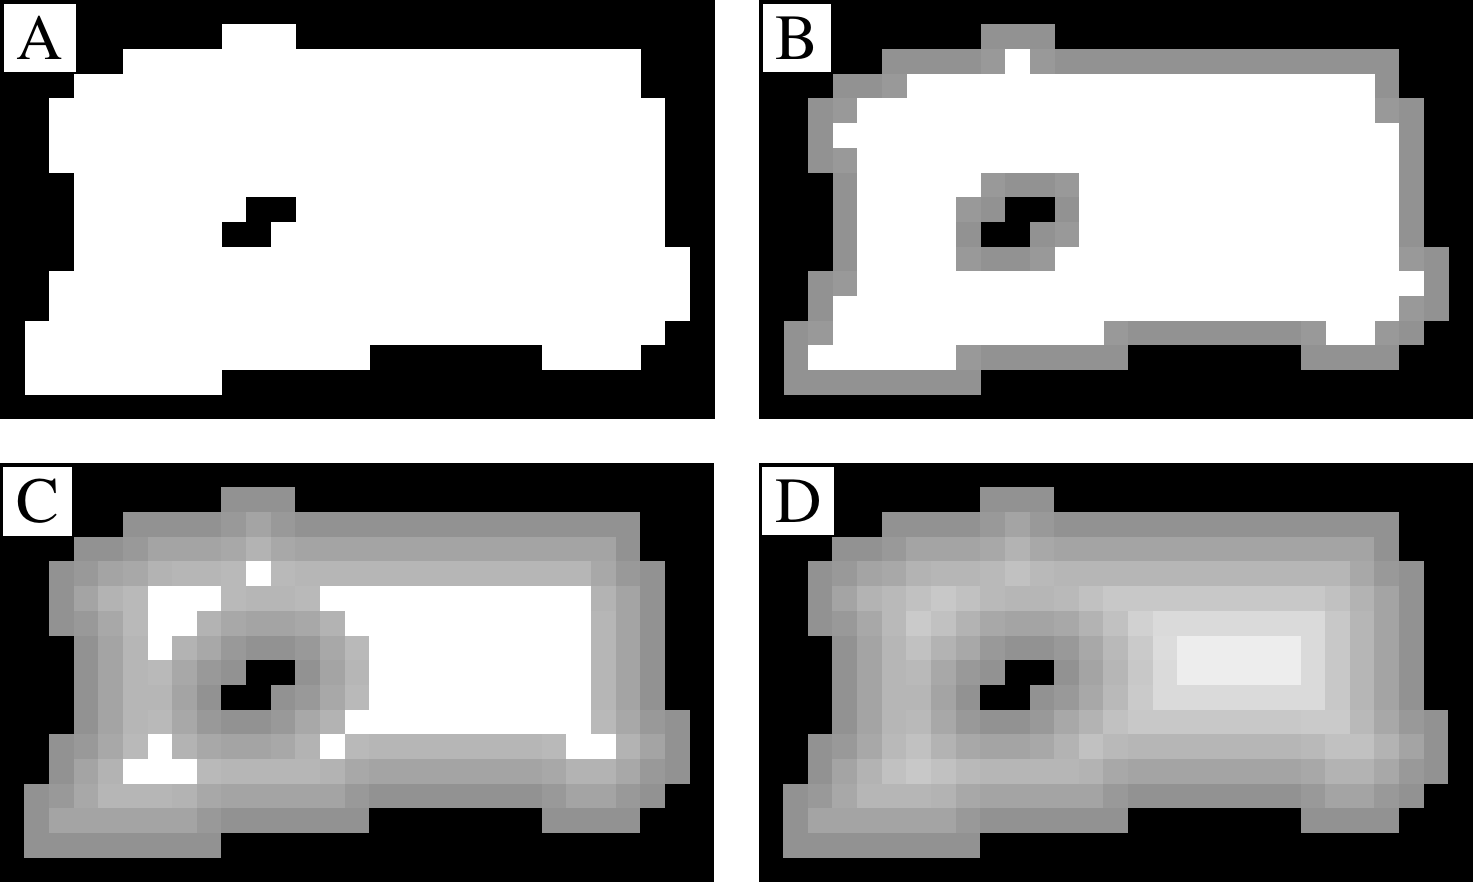
\includegraphics[width=1\linewidth]{imagenes/wavesBrush2Rows.png}
  \caption[Algoritmo brushfire.]{Algoritmo brushfire. (A) Los valores de distancia se inicializan con 0 (negro) para celdas ocupadas e infinito (blanco) para celdas vacías. (B) y (C) Las celdas ocupadas generan ondas que asignan distancias crecientes a medida que se propagan, indicadas por el aumento de brillo de las celdas. (D) Las ondas se detienen al no poderse reducir más valores de distancia. Una vez que se han detenido todas las ondas, se obtiene el mapa de distancia completo. Extraído de \cite{Lau2013}.}\label{fig:wavesBrush}
\end{figure} 
% \todo[inline]{mucho, recortar y colocar en el texto}

La ventaja sobre el método propuesto en \cite{wurm2008coordinated} es
que brushfire logra construir el GVD evitando el paso intermedio de
esqueletización. La idea se basa en asignar identificadores a cada
conjunto conexo de celdas ocupadas, y luego según la interpretación de
brushfire como ondas, las ondas provenientes de celdas ocupadas con
identificadores distintos colisionan en las celdas que deben pertenecer
al GVD. Notar que la asignación de identificadores presentada causa los
problemas asociados a generadores cóncavos comentados en la sección
\ref{subsec:GVD}, en la sección \ref{subsec:constGVDInc} se describe una
solución. 

\subsection{Construcción incremental de un GVD}\label{subsec:constGVDInc}
% A lo largo de la exploración el mapa construido recibirá, de forma frecuente, actualizaciones que solo modifican una pequeña porción del mismo. Dado esto, por motivos de eficiencia, se busca que los algoritmos que utilizan al mapa como una entrada eviten recomputarse completamente en cada actualización y que en su lugar actualicen el último resultado obtenido para que sea consistente con la última version del mapa.

% Los algoritmos que requieren recomputarse completamente al cambiar parte de la entrada son conocidos como \emph{algoritmos no incrementales}, por otro lado los algoritmos que actualizan la salida anterior a partir de los cambios experimentados desde la última entrada son llamados \emph{algoritmos incrementales}.

% Los algoritmos de generación de GVD, y de segmentación a partir de un GVD descritos anteriormente son no incrementales, por lo tanto dado el problema de eficiencia que esto implica es de interés describir variantes incrementales para los mismos.

A lo largo de la exploración el mapa construido recibe actualizaciones de forma frecuente que solo modifican una pequeña porción del mismo. Esto causa que los datos que tienen que ser consistentes con el mapa también deban actualizarse de forma frecuente. Dado esto, por motivos de eficiencia, se busca que los algoritmos que deben ejecutarse para mantener la consistencia de los datos con el mapa, eviten descartar el resultado anterior y recomputarse completamente en cada actualización, sino que en su lugar modifiquen el último resultado para que este sea consistente con la última version del mapa. 

La idea se basa en que, como se mencionó anteriormente, las actualizaciones son frecuentes pero también pequeñas y por lo tanto luego de una actualización gran parte del mapa se mantiene igual. Esto usualmente implica que gran parte del resultado anterior continua siendo valido luego de la actualización, solo siendo necesario modificar una pequeña porción del mismo para que este vuelva a ser consistente, lo cual suele ser órdenes de magnitud menos costoso que la alternativa de calcular todo desde cero. 
 % hecho de que las actualizaciones solo modificaron una  que e 

% Los algoritmos que requieren recomputarse completamente al cambiar parte de la entrada son conocidos como \emph{algoritmos no incrementales}, por otro lado los algoritmos que actualizan la salida anterior a partir de los cambios experimentados desde la última entrada son llamados \emph{algoritmos incrementales}.
Los algoritmos que actualizan el resultado anterior a partir de los cambios experimentados son llamados \emph{algoritmos incrementales}, en consecuencia los algoritmos que al cambiar parte de la entrada descartan el último resultado y recomputan el nuevo resultado desde cero se denominan como \emph{algoritmos no incrementales}.

El uso de algoritmos no incrementales como los presentados en la sección \ref{subsec:constGVD} no es adecuado cuando se desea mantener GVD asociado a un entorno que es actualizado en tiempo real mientras es explorado, para esto lo ideal es utilizar algoritmos incrementales. A continuación se describe el algoritmo incremental introducido en \cite{kalra2009incremental} denominado \emph{brushfire dinámico}, que como su nombre lo indica se basa en el algoritmo no incremental brushfire comentado en \ref{subsec:constGVD}.
% Los algoritmos de generación de GVD, y de segmentación a partir de un GVD presentados anteriormente no son incrementales, dado el problema de eficiencia que esto implica son de interés las variantes incrementales que se explicarán a continuación.

% , y por lo tanto su uso resulta ineficiente, por esto fueron desarrolladas variantes incrementales para los mismos.
% \subsubsection{Construcción incremental del GVD}
% El algoritmo incremental para la construcción de un GVD que se presentara en esta sección es conocido como \emph{brushfire dinámico}, formulado originalmente por \textit{et al.} en \cite{kalra2009incremental}. Este algoritmo se basa en el algoritmo no incremental \emph{brushfire}

% El algoritmo \emph{brushfire dinámico} es una variante incremental del algoritmo brushfire descrito hasta el momento presentada en \cite{kalra2009incremental}.

% Como se comento anteriormente, los algoritmos incrementales fundamentalmente consisten en tomar como entrada los cambios ocurridos desde la última ejecución, y a partir de estos modificar solo las porciones del último resultado necesarias para que vuelva a ser consistente. En este caso los cambios ocurridos corresponden a un conjunto de celdas en las que su estado pasa de ser ocupado a ser libre (se quita una celda ocupada) o viceversa (se agrega una celda ocupada). Y las porciones necesarias a modificar son las que al darse uno de los posibles cambios alteran la distancia mínima a un obstáculo calculada previamente. Cuando se quita una celda ocupada, son aquellas celdas que estaban más cerca de esta que de otra. Mientras que cuando se agrega una celda de ocupada, los cambios se dan en las celdas que pasan a tener esta nueva celda ocupada mas cerca que las demás.
Como se comento anteriormente, los algoritmos incrementales se basan en
mantener un resultado consistente con una entrada que sufre modificaciones a lo
largo del tiempo, solo actualizando las porciones del resultado que quedan
inconsistentes debido a dichas modificaciones.
En el contexto de brushfire dinámico los cambios en la entrada
corresponden a celdas cuyo estado pasa de ocupado a libre (se quita una
celda ocupada) o viceversa (se agrega una celda ocupada), mientras que las
porciones a actualizar son las celdas en las que la distancia
mínima a un obstáculo deja de ser consistente debido a los cambios.
Específicamente, cuando se quita una celda ocupada, es necesario actualizar
aquellas celdas que definen su mínima distancia a un obstáculo según la
celda que ahora se encuentra libre. 
Por otro lado cuando se agrega una celda ocupada, se deben actualizar las celdas 
cuya distancia a la nueva celda ocupada es menor que la distancia mínima a un
obstáculo que tenían antes de la modificación.

Brushfire dinámico lleva a cabo las actualizaciones propagando los cambios ocurridos
en forma de ondas. Las celdas $o$ que pasan a estar ocupadas emiten una onda
\say{consistente} que establece la distancia $dt_c$ recorrida por la onda a la
distancia $d_c$ asociada a la celda $c$ si $dt_{c}<d_{c}$, si la distancia se
modifica, entonces se establece a $o$ como el obstáculo a mínima distancia de $c$. En el
caso de las celdas $l$ que pasan a estar libres, se emana una onda
\say{inconsistente} que reinicia a $\infty$ las distancias $d_c$ de las celdas
$c$ que tienen a $l$ como obstáculo a mínima distancia, esta onda se expande
hasta llegar a alguna celda $c'$ que tiene un obstáculo valido a mínima
distancia. Al suceder esto desde $c'$ se resume la onda \say{consciente} que
causo su valor de distancia actual, y esta onda es la que establece la
distancia de las celdas previamente reiniciadas. En la figura
\ref{fig:wavesBrushDyn} se muestra gráficamente el funcionamiento de brushfire
dinámico.

\begin{figure}[H]
  \center
  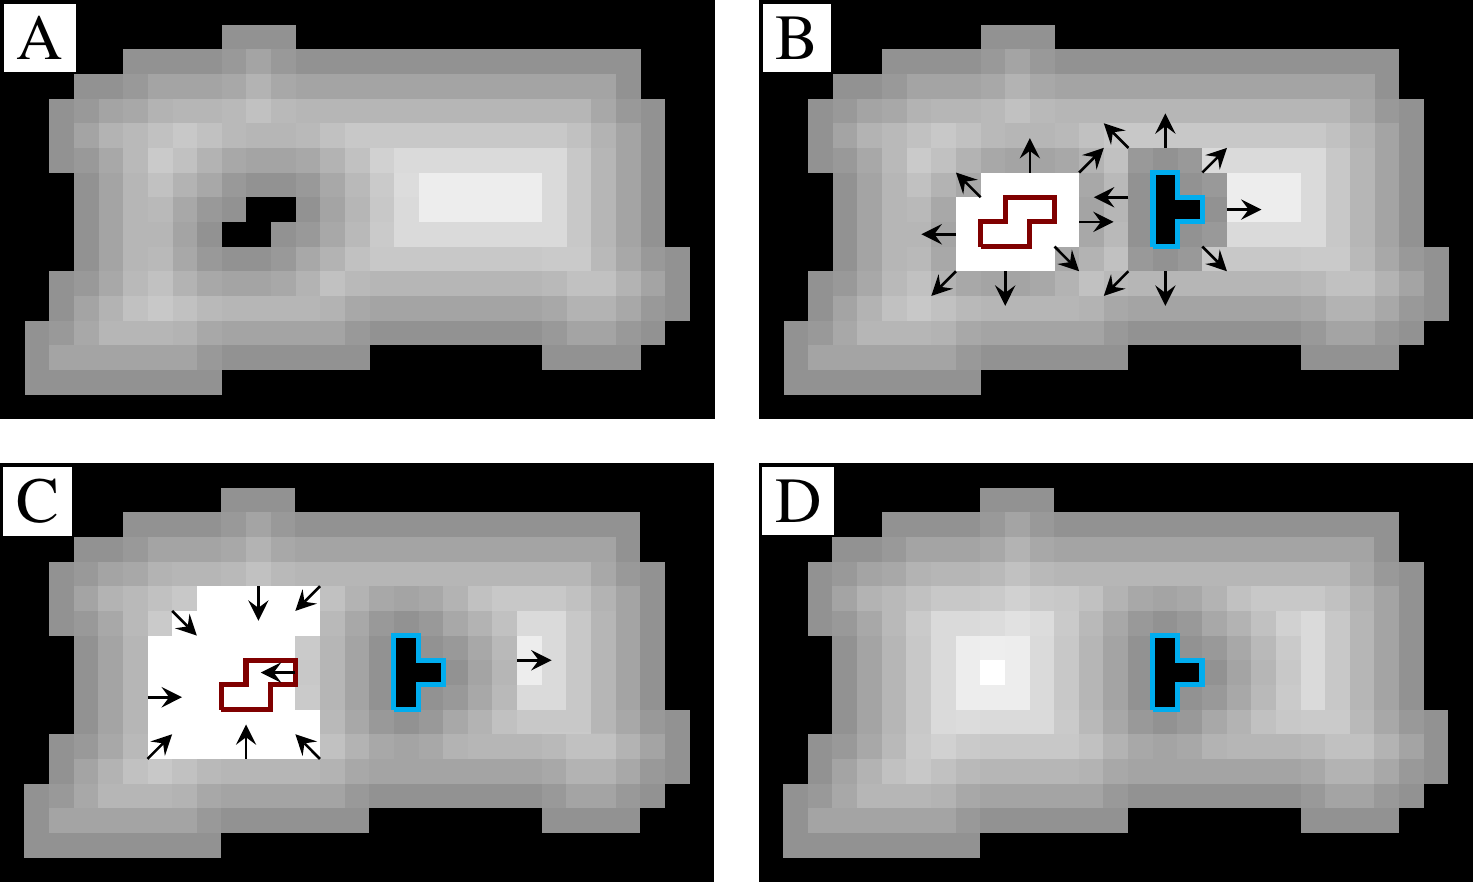
\includegraphics[width=1\linewidth]{imagenes/wavesBrushDinClean2Rows.png}
  \caption[Algoritmo brushfire dinámico.]{Algoritmo brushfire dinámico. (A) Último mapa de distancias calculado. (B) Un obstáculo es eliminado (contorno rojo) lo cual causa ondas inconsistentes que comienza a reiniciar los valores de distancia inválidos, a su vez un obstáculo es insertado (contorno azul) y generando ondas consistentes que propagan las nuevas distancias. (C) Cuando las ondas inconsistentes chocan contra celdas con un obstáculo más cercano válido estas se detienen y en ese mismo lugar inicia una onda consistente para restaurar los valores de distancia reiniciados. (D) Después que todas las ondas se detienen, la actualización se completa. Extraído de \cite{Lau2013}.}\label{fig:wavesBrushDyn}
\end{figure} 
% \todo[inline]{ídem fig anterior, recortar y colocar en el texto.}

%Con esto se tiene una definición de brushfire dinámico que calcula un mapa de distancia.
Al igual que en el algoritmo brushfire original, en brushfire dinámico la
construcción de un GVD se hace a partir de identificadores asignados a
conjuntos conexos de celdas ocupadas.
Las ondas consistentes en su expansion remueven las celdas del GVD, y al
detenerse agregan al GVD tanto las celdas en donde se detienen, como también
las celdas que causaron que se detengan, siempre y cuando dichas celdas tengan
identificadores distintos entre sí. Por otro lado las ondas inconsistentes remueven del
GVD a todas las celdas cuya pertenencia al GVD involucra a celdas previamente
ocupadas que pasaron a ser libres. Un ejemplo de como agregar y remover un
obstáculo altera al GVD se encuentra en la figura \ref{fig:ejWavesIncKarlra}. 

\begin{figure}[H]
  \center
  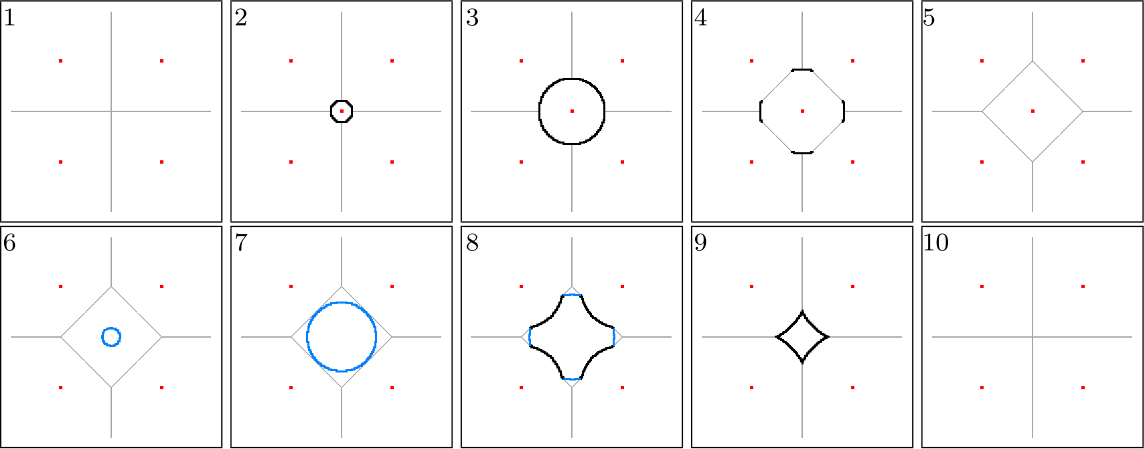
\includegraphics[width=1\linewidth]{imagenes/wavesKalra.png}
  \caption[Olas de brushfire dinámico.]{Una secuencia que ejemplifica las olas generadas cuando se agregan obstáculos (1-5) y se eliminan obstáculos (6-10). (1-5) Se agrega nueva celda ocupada en el centro del entorno (en rojo) lo cual produce una ola consistente (en negro) que al detenerse genera celdas pertenecientes al GVD (en gris). (6-10) La celda central deja de ser un obstáculo produciéndose una ola inconsistente (en azul) que remueve las celdas del GVD que involucran a la celda ocupada que paso a ser libre mientras que al al llegar a cedas con una distancia mínima generar olas inconsistentes (en negro) que reparan el GVD. Extraído de \cite{kalra2009incremental}.}\label{fig:ejWavesIncKarlra}
\end{figure} 


De esta forma se logra la construcción incremental de un GVD. Sin embargo en \cite{Lau2013} se destaca algunas problemáticas de brushfire dinámico, principalmente que el GVD generado tiene líneas de dos celdas de ancho y que no genera pertenencia al GVD en el interior de obstáculos cóncavos como lo son habitaciones con una sola entrada, lo cual es crítico en entornos estructurados. Los problemas mencionados se pueden ver a la izquierda de la figura \ref{fig:lauPalo}.

Para solucionar las problemáticas planteadas Lau \textit{et al.}
proponen cambios al algoritmo de brushfire dinámico. El problema de
generación de GVD en obstáculos cóncavos se relaciona con el uso de
conjuntos conexos de obstáculos para determinar la pertenencia de celdas
al GVD (sección \ref{subsec:GVD}). Dado esto la solución propuesta
consiste en dejar de utilizar identificadores para los conjuntos conexos
de obstáculos, en su lugar utilizar un identificador para cada celda
ocupada. Y al chocar dos olas, las celdas en donde se da el choque
pertenecen al GVD si sus identificadores de obstáculo a mínima distancia
son distintos y las celdas ocupadas correspondientes a dichos
identificadores no son adyacentes en la grilla. Este cambio soluciona la
generación del GVD en obstáculos cóncavos. Con respecto a las líneas de
dos celdas de ancho la propuesta consiste en aplicar técnicas que
permitan eliminar las celdas redundantes, estas son la celdas del GVD
que son adyacentes a más de una celda perteneciente al GVD (no son
hojas) y que su remoción no desconecta al GVD. A la derecha de la figura
\ref{fig:lauPalo} se muestra el resultado de aplicar estos cambios.

\begin{figure}[H]
  \center
  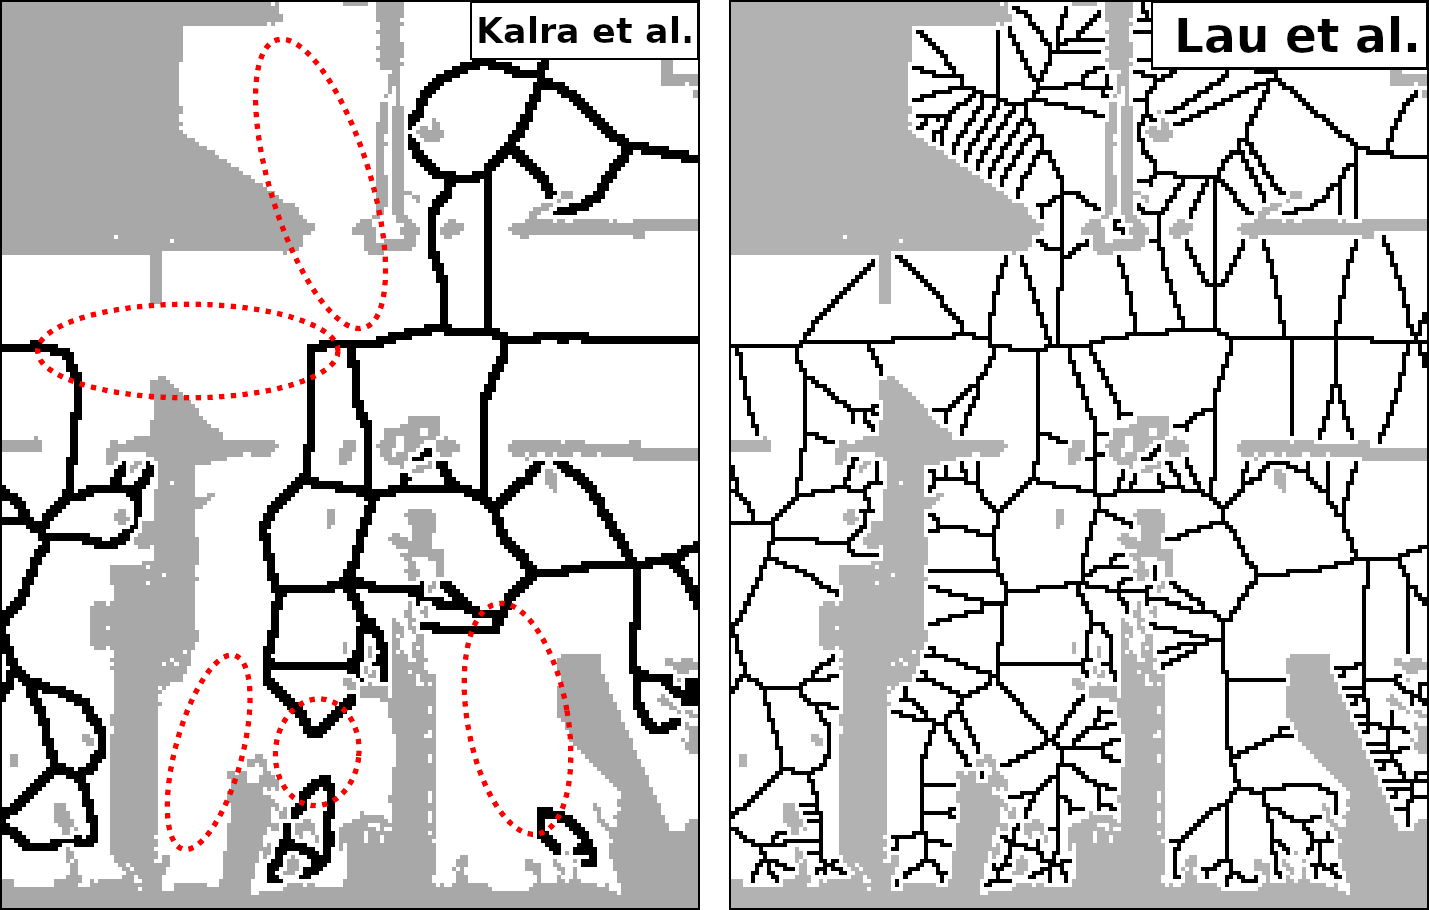
\includegraphics[width=0.75\linewidth]{imagenes/lauPalo.png}
  \caption[Resultados de brushfire dinámico original y la variante propuesta por Lau \textit{et al.}]{Resultados de brushfire dinámico original (a la izquierda) y la variante propuesta por Lau \textit{et al.} (a la derecha). Las elipses marcan los lugares en donde el acercamiento de Kalra \textit{et al.} falla al no generar celdas pertenecientes al GVD. Extraído de \cite{Lau2013}.}\label{fig:lauPalo}
\end{figure} 


% \todo[inline]{uniformizar captions, sacar 'Ejemplo de'. además reescribiría los captions b) y c): Mapa original y mapa de distancias (color proporcional a la distancia al obstáculo más cercano). Mapa original y GVD (resultante de la esqueletización)}
% \begin{figure}[H]
%   \begin{center}
%   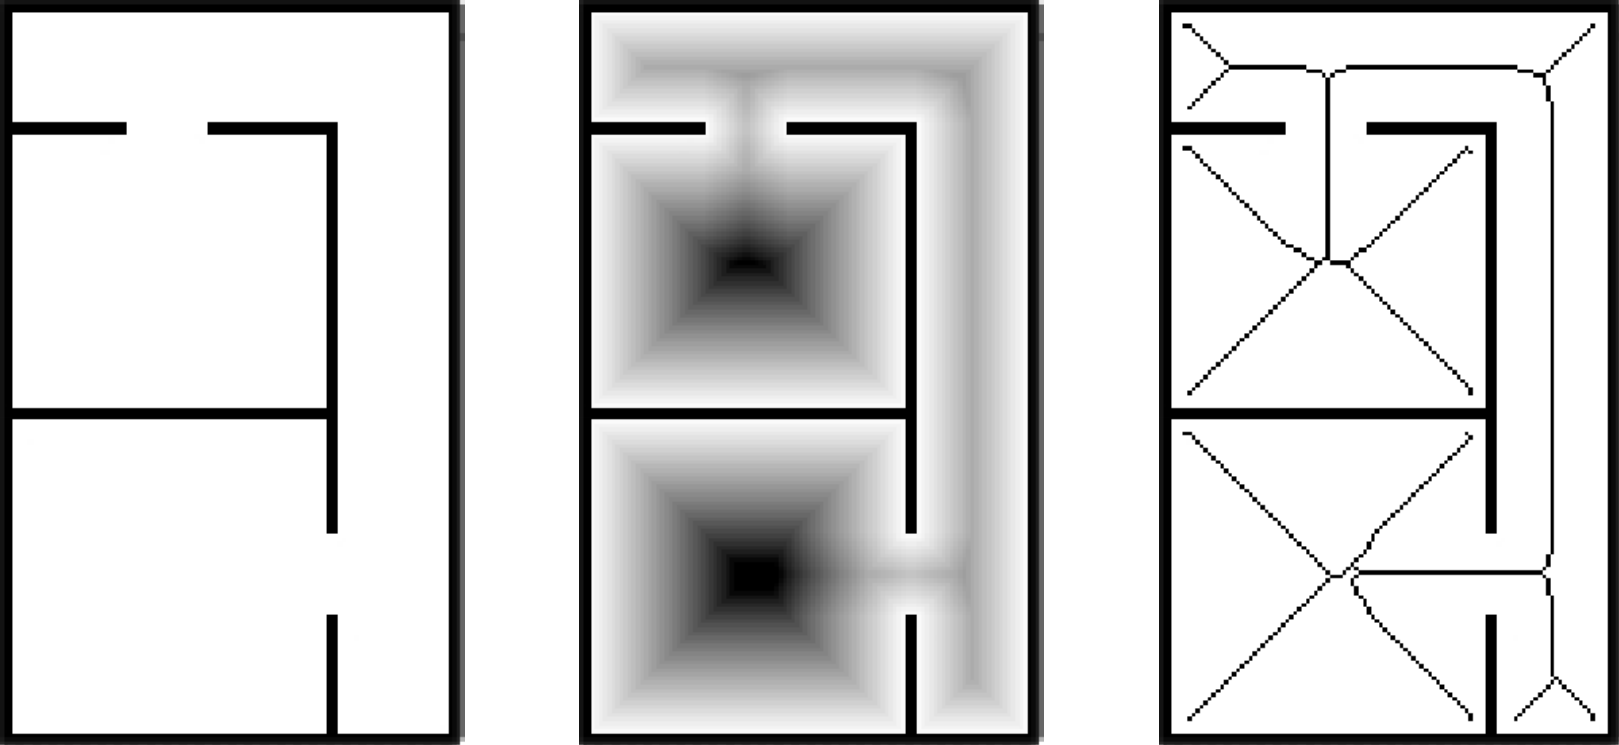
\includegraphics[width=7.5cm]{imagenes/wurmGVD.png}
%   \end{center}
%   \caption{Ejemplo del método de construcción de un GVD basado en grilla extraído de \cite{wurm2008coordinated}. A la izquierda se encuentra el mapa original, en el centro el mapa original junto a su correspondiente mapa de distancia (cuanto más oscuro es un punto, mayor es la distancia al obstáculo más cercano). A la derecha se encuentra el mapa original junto al resultado de la esqueletización del mapa de distancia (líneas negras) que es a su vez el GVD construido.}\label{fig:wurmGVD}
% \end{figure} 

% La esqueletización es usada en lugar de s
% Este método evita problemas que se pueden dar al generar un GVD discretizado a partir de la definición de pertenencia al GVD directamente adaptada a un espacio discretizado en celdas, donde una celda pertenece al GVD si tiene dos o mas celdas ocupadas a una misma distancia. Un ejemplo de este tipo de problemas es el que se genera en los corredores cuya discretización tiene una cantidad par de celdas entre sus paredes, en este caso si se aplica la definición de GVD a las celdas ninguna debería pertenecer al GVD dado que ninguna celda tendría una misma distancia a dos celdas ocupadas (paredes del corredor). Este comportamiento no es deseable ya que se debe a una discretización particular del espacio, si el tamaño de las celdas fuera otro y en lugar de ser un numero par fuera uno impar se tendría un GVD a lo largo del centro del corredor, y mas importante aun, un GVD sobre un corredor en un espacio continuo siempre genera una linea sobre el centro del corredor. %El método de \cite{wurm2008coordinated} soluciona este tipo de problemas porque la esqueletización asegura la generación de puntos pertenecientes al GVD en las 

% \begin{figure}
%   \centering
%   \subfloat[Ancho par]{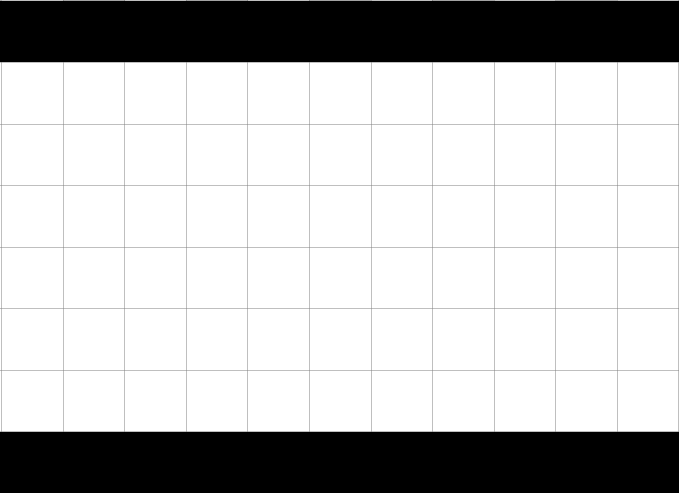
\includegraphics[clip=true, width=0.45\linewidth]{imagenes/anchopar.png}
%   \label{map:laberinto}}
%   \subfloat[Ancho impar]{\hspace{0.1\linewidth}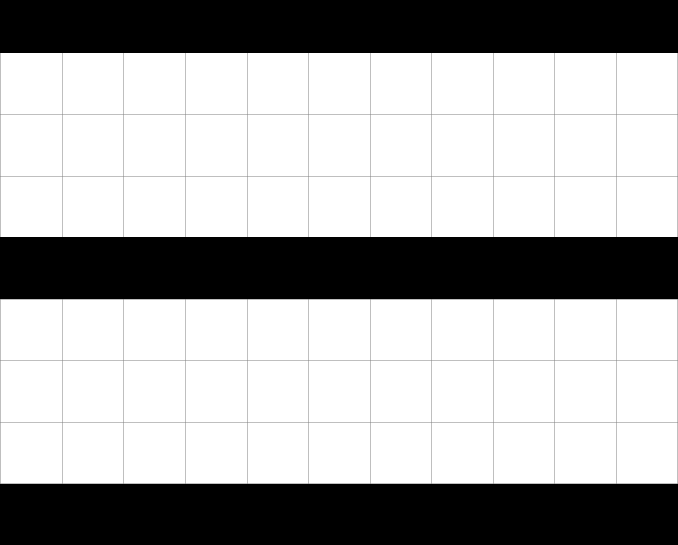
\includegraphics[clip=true, width=0.45\linewidth]{imagenes/anchoimpar.png}
%   \label{map:office}}
%   \caption{Entornos}
% \end{figure}

\subsection{Generación de mapas topológicos basados en regiones a partir de un GVD}\label{subsec:mapaTopGVD}
En \cite{Thrun1998} se propone un método que permite, a partir de un GVD generado a través de una grilla de ocupación, segmentar el entorno en habitaciones y corredores, con el objetivo de generar un mapa topológico cuyas regiones de interés serán los segmentos reconocidos. La idea principal del algoritmo de segmentación es que las entradas y salidas entre los segmentos son pasajes estrechos, y por lo tanto encontrar estos pasajes estrechos permite delimitar segmentos.

Para describir el método de segmentación es necesario introducir tres nuevos conceptos asociados al $\mli{GVD}$, el primero es el concepto de \emph{despeje} (del ingles clearance) $D : W \rightarrow R$ de un punto $p \in W$, que corresponde a la distancia del punto $p$ al punto ocupado más cercano. De de ser $p \in \mli{GVD}$ el despeje equivale a la distancia entre $p$ y alguno de sus generadores base generalizados $\mli{GBG}_p$ (recordar que todos están a una misma mínima distancia de $p$ \eqref{eq:GBG}). El segundo es el concepto de \emph{puntos críticos} $C \subset \mli{GVD}$, que son los puntos pertenecientes al GVD que minimizan el despeje localmente en el GVD, esta definición se formaliza en \eqref{eq:crit}, donde $d_p(p')$ es la distancia entre $p$ y $p'$. 
\begin{equation}
  % p\ \in C \iff p \in \mli{GVD}\ \land \ D(p) < D(p')\ \forall p' \in Ady(p) 
  C = \{p\ \in \mli{GVD} : \exists \upvarepsilon > 0, \forall p' \in \mli{GVD}, d_p(p') \leq \upvarepsilon, D(p) < D(p') \} \label{eq:crit}
\end{equation}
El tercer y último concepto es el de \emph{líneas críticas}, que son las líneas
que se encuentran entre un punto crítico $p \in C$ y los puntos más cercanos de
sus generadores base generalizados $\mli{GBG}_p$. La figura \ref{fig:crits}
ilustra estos conceptos.

\begin{figure}[H]
  \center
  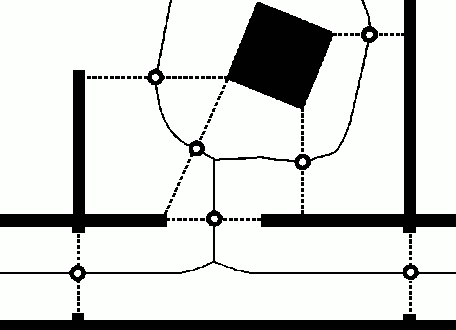
\includegraphics[width=0.75\linewidth]{imagenes/CritsSharpMono.png}
  \caption[Puntos críticos y lineas críticas.]{Puntos críticos y líneas críticas. Los puntos críticos se indican con círculos y las líneas críticas con líneas punteadas. Notar que el despeje en puntos críticos se corresponde con el largo sus líneas críticas asociadas. Extraído de \cite{Thrun1998}.}\label{fig:crits}
\end{figure} 



El algoritmo comienza determinando el estado (ocupado o libre) para cada celda de la grilla de ocupación, para esto se define previamente un umbral de probabilidades, y si la probabilidad de ocupación de una celda supera dicho umbral se considera como ocupada y de lo contrario sera considerada como libre. Con la nueva grilla de estados determinados se procede a construir su  GVD. Luego se encuentran los puntos críticos asociados al GVD construido para luego obtener las líneas críticas para cada punto crítico encontrado. Finalmente los segmentos serán las regiones de espacio libre delimitadas por las líneas críticas y los obstáculos. En la figura \ref{fig:ejThrunTop} se muestra un ejemplo de algunas etapas del algoritmo aplicado a un mismo entorno.

\begin{figure}[H]
  \centering
  \subfloat[GVD]{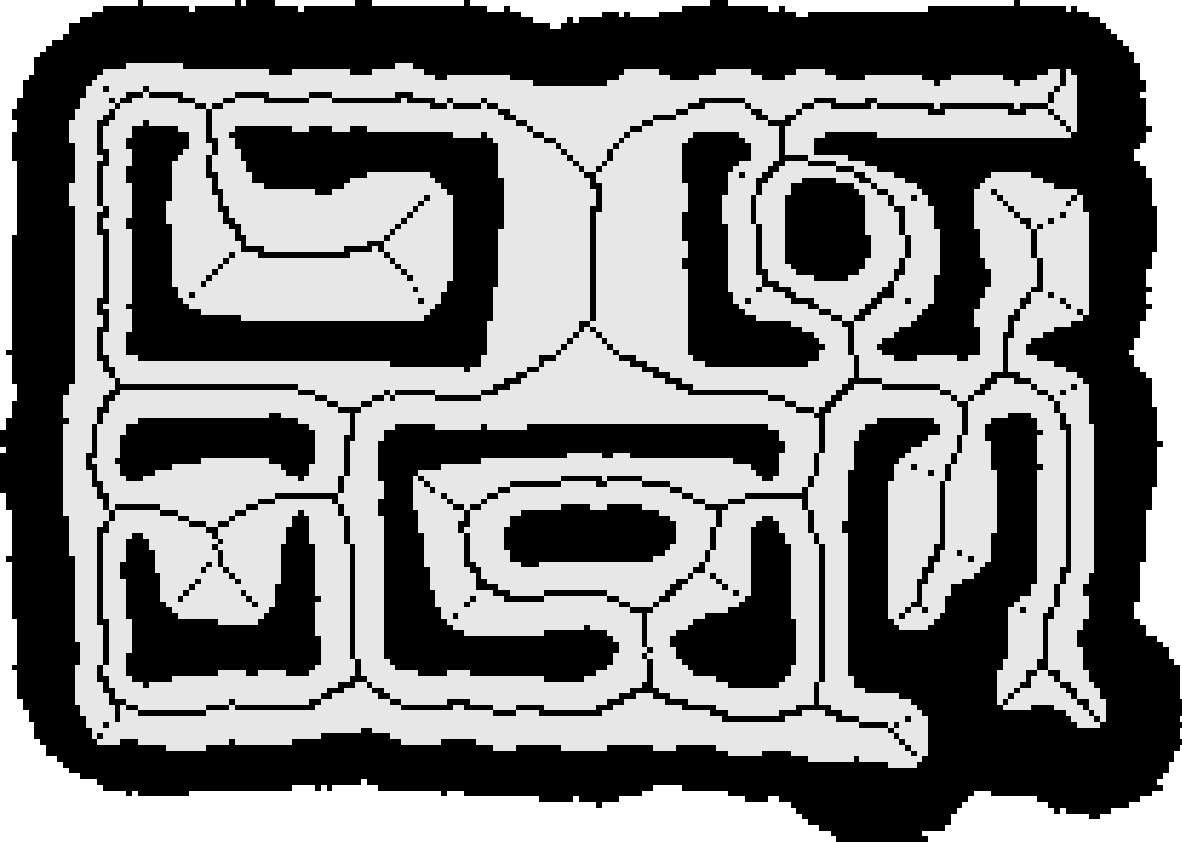
\includegraphics[clip=true, width=0.45\linewidth]{imagenes/thrunTop/a.png}\label{fig:ejThrunTopA}}
  \qquad
  \subfloat[Lineas criticas]{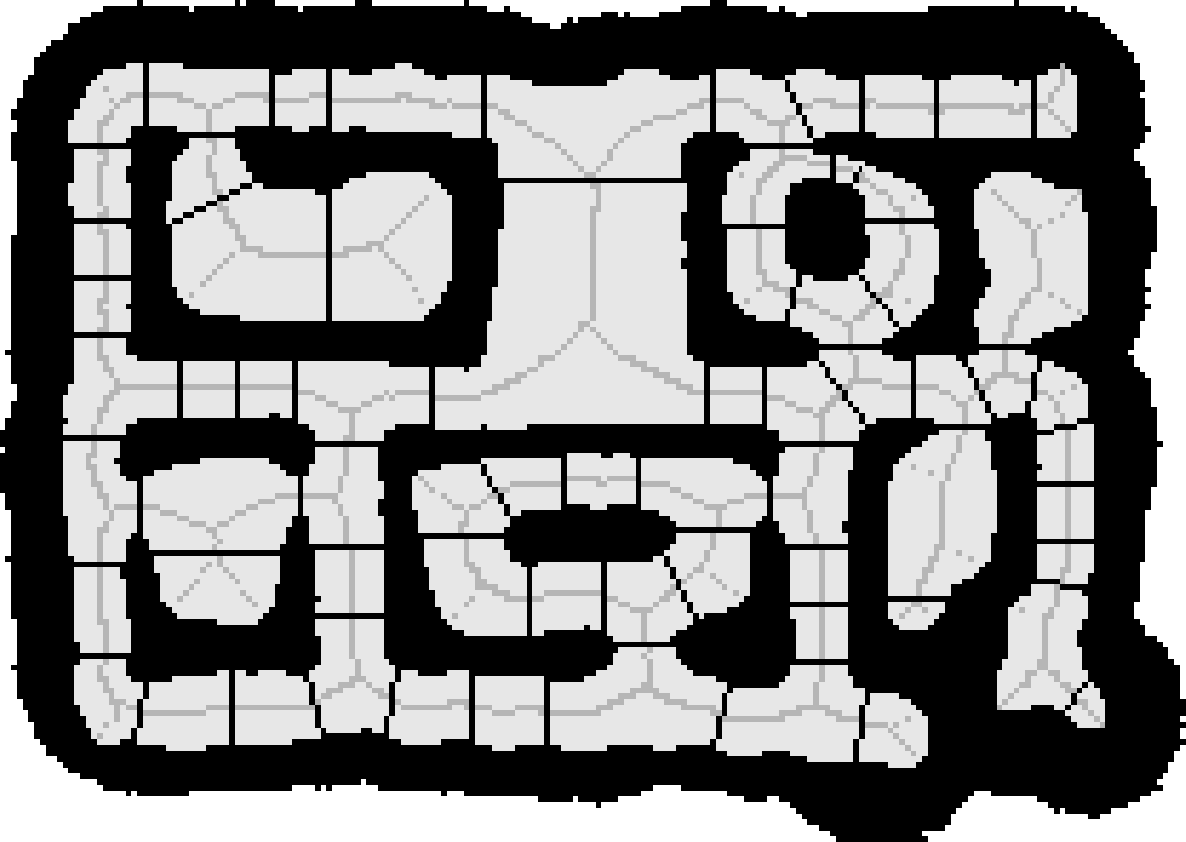
\includegraphics[clip=true, width=0.45\linewidth]{imagenes/thrunTop/b.png}\label{fig:ejThrunTopB}}
  \qquad
  \subfloat[Regiones]{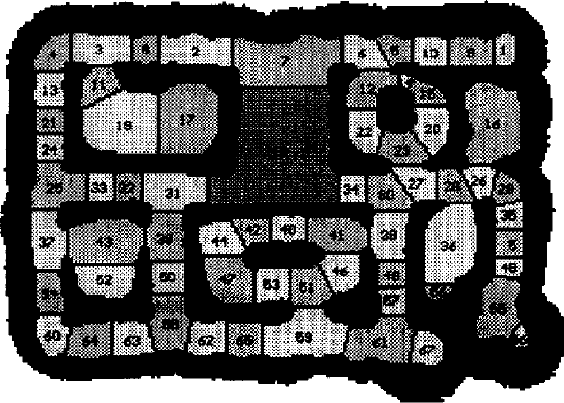
\includegraphics[clip=true, width=0.45\linewidth]{imagenes/thrunTop/c.png}\label{fig:ejThrunTopC}}
  \qquad
  \subfloat[Mapa topologico]{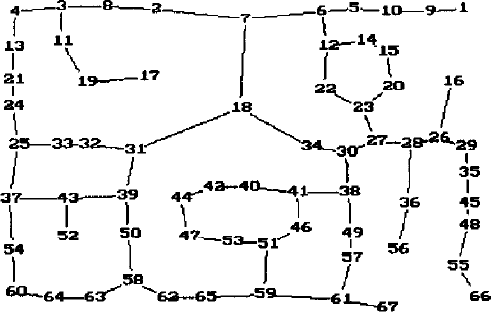
\includegraphics[clip=true, width=0.45\linewidth]{imagenes/thrunTop/d.png}\label{fig:ejThrunTopD}}
  \caption[Método de construcción de un mapa topológico basado en regiones a partir de un GVD.]{Método de construcción de un mapa topológico basado en regiones a partir de un GVD. Los números de las figuras (c) y (d) son identificadores arbitrarios de regiones. Extraído de \cite{Thrun1998}.}\label{fig:ejThrunTop}
\end{figure}
% \todo[inline]{sacar 'Ejemplo de', además hay que editar estas imgs limpiando los fondos blancos. a y b seguro, la c capaz se puede dejar}

La idea subyacente de este algoritmo es que, por definición, los puntos críticos se encuentran presentes en el centro de todo pasaje estrecho siendo los puntos obstaculizados más cercanos los extremos de dicho pasaje. Por lo tanto las líneas críticas estarán ubicadas a lo largo de cada pasaje estrecho y dada la consideración que las transiciones entre los segmentos se dan en los pasajes estrechos, las líneas críticas actúan naturalmente como limites entre cada segmento.

% TODO describir bien el algoritmo no incremental de Liu ming (capaz despues)

En \cite{wurm2008coordinated} los autores argumentan que la propuesta original de Thrun tiene el problema de generar gran cantidad de puntos críticos que no se encuentran en un pasaje entre segmentos, considerados como falsos positivos que generan una segmentación excesiva del entorno (un ejemplo de este problema se puede ver en la cantidad de segmentos generados en los corredores de la figura \ref{fig:ejThrunTopC}). Entonces, con el motivo de evitar los mencionados falsos positivos y mejorar la segmentación generada agregan condiciones adicionales a la definición de punto crítico original, estas son que el vértice asociado a un punto crítico en el grafo que representa GVD debe ser de grado 2 y tener un vecino de grado 3 (un vértice de intersección entre varios caminos)\todo{convendría colocar una imagen que muestre la mejora}. 

\subsection[Alternativas para la generación de mapas topológicos basados en regiones]{Alternativas para la generación de mapas topológicos basados en regiones}\label{subsec:mapaTopAlt}

Existen alternativas para generar mapas topológicos basados en regiones, que no
involucran el uso de un GVD.

En \cite{Fermin-Leon2017} la generación se logra interpretando la grilla de
ocupación como una imagen binaria, para luego extraer sus contornos los cuales
se representan como polígonos. Finalmente se aplica un algoritmo que segmenta
el espacio según la convexidad de dichos contornos, obteniendo así un mapa
topológico basado en regiones.

Por otro lado en \cite{zivkovic2006hierarchical} se interpreta la grilla de
ocupación como un grafo donde cada celda libre es un nodo y las aristas se
encuentran entre nodos cuyas celdas asociadas son adyacentes en la grilla.
Usando un método de particionamiento de grafos se obtienen agrupaciones de
nodos que corresponden a las regiones del mapa topológico construido.

En \cite{martinez2006semantic} se presenta un método de generación basado en
aprendizaje automático. En cada celda libre de la grilla de ocupación se
determina el valor de atributos geométricos asociados a la distancia de la
celda a los obstáculos que tiene a su alrededor. Estos atributos se utilizan
para entrenar un modelo de clasificación denominado \emph{AdaBoost}
\cite{schapire1999improved} que es usado para clasificar celdas libres en
categorías semánticas como por ejemplo puerta, habitación o corredor. Luego en
la practica a partir de los valores de los atributos y el modelo entrenado se
clasifica cada celda libre. Las regiones que conforman el mapa topológico se
obtienen agrupando las celdas con una misma categoría. La figura
\ref{fig:ejMartinezTop} muestra un ejemplo de la clasificación y su posterior
segmentación.

\begin{figure}[H]
  \centering
  \subfloat[Clasificación]{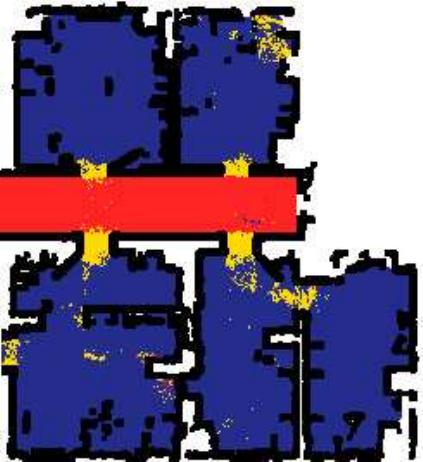
\includegraphics[clip=true, width=0.2\linewidth]{imagenes/aa_clas.png}}
  \qquad
  \subfloat[Mapa topológico]{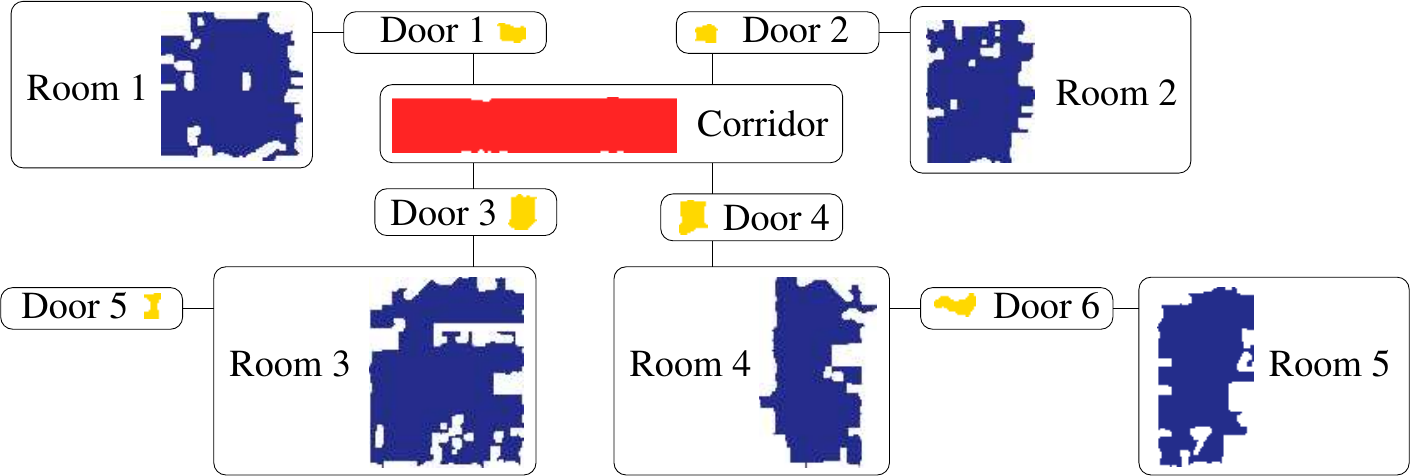
\includegraphics[clip=true, width=0.7\linewidth]{imagenes/aa_topo.png}}
  \caption[Método de construcción de un mapa topológico basado en regiones a partir de aprendizaje automático.]{Método de construcción de un mapa topológico basado en regiones a partir de aprendizaje automático. Las celdas tienen un color correspondiente a su clasificación, amarillo corresponde a puerta, azul a habitación y rojo a corredores. Extraído de \cite{martinez2006semantic}.}\label{fig:ejMartinezTop}
\end{figure}

% Un comentario relevante sobre los métodos basados en aprendizaje automático es
% que para obtener buenos resultados los clasificadores deben ser entrenados con
% cantidades suficientes de datos representativos de los entornos a segmentar. Lo
% cual puede ser un inconveniente si se segmentan nuevos entornos con
% caracteristicas no contempladas los utilizados para entrenar. 

\subsection{Criterios de calidad de un mapa topológico basado en regiones}
\subsubsection{Criterio de calidad basado en intuiciones geométricas}
% un mapa topológico basado en regiones se considera útil si
% representa la estructura del entorno de manera correcta y eficiente.
En \cite{Liu2015} se plantea un criterio para cuantificar la calidad de un mapa
topológico basado en regiones mediante indicadores que surgen de intuiciones
geométricas. El criterio considera tanto la calidad de cada región de forma
independiente, como la calidad de la segmentación formada por todas las
regiones en su conjunto.

La \textbf{calidad de una región} se calcula tomando en cuenta dos indicadores
la convexidad y la compacidad. 

La \emph{convexidad} indica la similitud entre la región y su envolvente
convexa. Se calcula como el cociente entre el área de la región y el área de
su envolvente convexa. 

La \emph{compacidad} mide la distribución de una región con respecto
a su centro de masa. A menor valor de compacidad mayor es la concentración de
una región sobre su centro de masa.

La \textbf{calidad de segmentación} se compone de varios indicadores de
calidad sobre ciertas características globales de la segmentación. Estos indicadores son la
cobertura, validez y simplicidad.

% En el caso ideal cada punto del entorno esta asociado a una región en el mapa
% topológico, pero por diversas razones este puede no ser el caso. Dado esto se define
La \emph{cobertura} de una segmentación se define como el cociente entre la
suma de las áreas de cada región y el área total del mapa.

La \emph{validez} indica la proporción de regiones validas en la segmentación, siendo valida una
región cuando esta es accesible por los robots utilizados.

% Por lo tanto, es útil penalizar las soluciones con
% un gran número de regiones. Por otro lado, si el número de regiones es
% demasiado pequeño, la segmentación no tendrá sentido.

La \emph{simplicidad} es un valor que busca penalizar a las segmentaciones que
sean demasiado complejas o demasiado simples, esto se logra midiendo la
diferencia entre la cantidad de regiones de la segmentación generada y la 
cantidad de regiones esperada para el entorno actual.

Finalmente la \textbf{calidad de un mapa topológico basado en regiones} se
reduce a combinar aritméticamente la calidad de cada región y los indicadores
de calidad de la segmentación.


\subsubsection{Criterio de calidad basado en la segmentación humana}
En \cite{bormann2016room} se propone que la calidad de una segmentación
corresponde a su semejanza a la segmentación humana y se proporciona un metodo
para medirla.  

En el contexto del articulo la segmentación humana se aproxima como la
segmentación que un humano genera para dicho entorno. Luego para cuantificar la
semejanza se definen dos indicadores, exhaustividad y precision. 

La \emph{exhaustividad} se define como el área correspondiente a la mayor 
superposición entre una región de la segmentación humana y una región de la
segmentación evaluada, dividida por el área de la región de la segmentación
humana. La exhaustividad es alta si las regiones de la segmentación humana
están completamente contenidas en las regiones de la segmentación evaluada. 

La \emph{precisión} de manera similar se define como el área correspondiente a
la mayor superposición entre una región de la segmentación humana y una región
de la segmentación evaluada, dividida por el área de la región de la
segmentación evaluada. La precisión es alta si las regiones de la segmentación
evaluada están completamente contenidas en las regiones de la segmentación
humana . 

En la subsegmentación, la exhaustividad es alta y la precisión es baja,
mientras que en la sobresegmentación, la precisión es alta y la exhaustividad
es baja.  Solo si ambas medidas son altas, la segmentación evaluada se ajusta
bien a la segmentación humana.  

Este criterio es utilizado en \cite{bormann2016room,Fermin-Leon2017}
para comparar las segmentaciones resultantes de distintos acercamientos para la
construcción de mapas topológicos basados en regiones, incluyendo el método
descrito en \ref{subsec:mapaTopGVD} y algunos de los mencionados en
\ref{subsec:mapaTopAlt}, siendo la segmentación a partir de un GVD la que
obtiene mejores resultados en general.  

% \subsection{Criterios de calidad de un mapa topológico basado en regiones}
% Según \cite{Liu2015} un mapa topológico basado en regiones se considera útil si representa la estructura del entorno de manera correcta y eficiente. Para ello, consideran dos criterios principales, la calidad asociada a cada region y la topología la segmentación. Los criterios propuestos se basan principalmente en intuiciones geométricas. 

% \subsubsection{Calidad de una region}
% Los autores determinan que existen dos aspectos que intervienen en la calidad de una region, la convexidad $c_i$ y la compacidad $s_i$, específicamente, definiendo la calidad de una region como $q_i = c_i - s_i$. Adicionalmente se menciona que tanto $c_i$ como $s_i$ pueden ser multiplicados por pesos en el calculo de $q_i$ para  para hacer énfasis en una u otra característica.

% \paragraph{Convexidad}
% Esta se puede representar como el cociente entre el área de la region y el área de su envolvente convexa. La envolvente convexa de una region se define como el polígono convexo de menor área que contiene a la region. Un polígono convexo cumple que para cualquier par de puntos que pertenecen a la frontera del polígono, el segmento de recta que los conecta estará contenido en dicho polígono. Entonces sea $A_i$ el área de la region $R_i$ y $H_i$ el área de su envolvente convexa, la convexidad para esta region sera:
% \begin{equation}
%   c_i=\frac{A_i}{H_i}
% \end{equation}
% Se cumple que $A_i \leq H_i$ siendo iguales cuando la region es convexa, por lo tanto $c_i$ sera igual a uno cuando la region es convexa, y su valor disminuirá entre más difiera el área de la region con la de su componente convexa. En la figura \ref{fig:ejemplConvexidad} se muestra a modo de ejemplo el valor de convexidad $c$ asociado a dos regiones con distinta convexidad.
% \begin{figure}[H]
%   \centering
%   \subfloat[c=0.88]{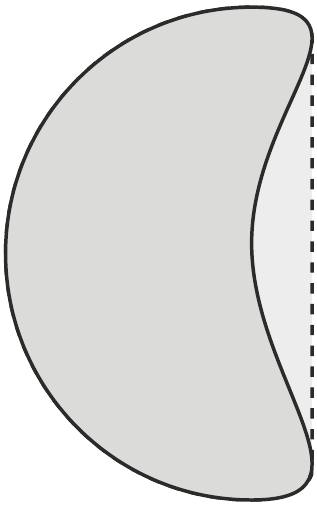
\includegraphics[clip=true, height=0.25\linewidth]{imagenes/liuConv/a.png}}
%   \hspace{2cm}
%   \qquad
%   \subfloat[c=0.56]{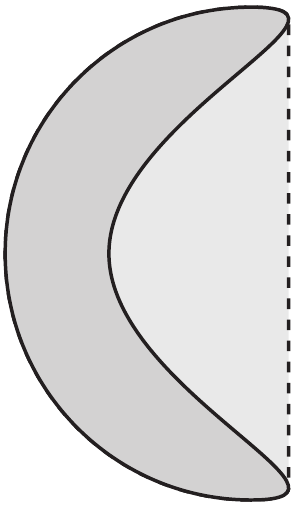
\includegraphics[clip=true, height=0.25\linewidth]{imagenes/liuConv/b.png}}
%   \caption[Regiones convexas y su valor de convexidad asociado.]{Regiones convexas y su valor de convexidad asociado. Las líneas sólidas delimitan las regiones y las punteadas sus envolventes convexas. Extraído de \cite{Liu2015}.}\label{fig:ejemplConvexidad}
% \end{figure}
% % \todo[inline]{conviene utilizar captions más cortos. ej. Regiones convexas. Las líneas sólidas delimitan las regiones y las punteadas sus envolventes convexas. además, delante de la llaves, en la defición del caption, conviene agregar entre paréntesis rectos el 'nombre' de la figura. esto será tomado para generar el índice de figuras de modo que no te queden entradas quilométricas}

% \paragraph{Compacidad}
% % Cuanto mas cercanos son los puntos que componen una region a su centro mas compacta sera la region.
% La compacidad de una region mide la distribución una region con respecto a su centro de masa. La compacidad $s_i$\todo{$s_i$ ya se usaba para los generadores de V} de una region $R_i$ se calcula a partir de una discretization de dicha region en celdas de dimensiones y peso uniforme, llamadas elementos de masa. En \eqref{ec:compacidad} se define la compacidad $s_i$ para un region $R_i$, donde $x_j$ e $y_j$ son las coordenadas $x$ e $y$ de los elementos de masa\todo{qué sería un elemento de masa? una molécula? un átomo?} de $R_i$, $M_i$ es igual a la cantidad de dichos elementos de masa y $x_0$ e $y_0$ son las coordenadas del centro de gravedad\todo{de masa?} de $R_i$.
% \begin{equation}
%   s_i=\frac{1}{M_iA_i}\sum_j \frac{(x_j-x_0)^2 + (y_j-y_0)^2}{A_i} \label{ec:compacidad}
% \end{equation}
% \todo[inline]{si $M_i$ es igual a la suma de esos elementos, los elementos tienen masa elemental/unitaria. pero eso es menos genérico que considerar que cada elemento podría tener masa $m_i$ distinta y que $M_i=\sum m_i$. en ese caso, la masa $m_i$ debería multiplicar a cada término de la sumatoria. lo que nos lleva a una definición muy alineada con la de centro de masa. por otro lado, $A_i$ ya está dividiendo afuera, no creo que vaya también en la sumatoria. además, unidades no cierran. asumo que la compacidad no tiene unidad y para ello falta que aparezca la masa en el numerardor. finalmente, me parece raro que no aparezca el volumen. o en realidad, no se para qué aparece la masa.}
% Notar que cuanto mas compacta sea una region menor sera su valor $s_i$ (si se entiende por region compacta una region en la cual sus puntos interiores son cercanos al centro de masa).

% \subsubsection{Calidad de segmentación}
% Para determinar la calidad general de la segmentación, sera necesaria, ademas de la calidad de cada region, la calidad de las características globales de la segmentación. Para lograr determinar dichas características se definen varios indicadores que se mencionarán a continuación.

% \paragraph{Cobertura}
% En el caso ideal cada punto del entorno esta asociado a una region en el mapa topológico, pero por diversas razones este puede no ser el caso. Dado esto se define la cobertura $C$ de una segmentación como el cociente del área representada por el mapa topológico y el área del mapa:
% \begin{equation}
% C=\frac{\sum^N_{i=1} A_i}{A_m}
% \end{equation}
% Donde $A_m$ es el área total del mapa y $N$ es el numero de regiones.

% \paragraph{Validez}
% La validez $V$ de una segmentación se define como el cociente entre el numero de regiones validas y el numero total de todas las regiones:
% \begin{equation}
%   V=\frac{\#regiones\ validas}{\#total\ de\ regiones}
% \end{equation}
% Se considera que una region valida debe ser accesible por los robots utilizados. Teniendo esto en cuenta una region será valida si cubre un área mayor a $A_{min}$ y tiene al menos una entrada de ancho mínimo $l_{min}$, siendo los valores $l_{min}$ y $A_{min}$ definidos a partir las dimensiones de los robots utilizados.\todo{entiendo entonces, que según este indicador, un alg de segmentación es mejor si logra 'filtrar' segmentos inaccesibles}

% \paragraph{Simplicidad}
% Una de las ventajas principales de los mapas topológicos es su simplicidad, que permite ayudar a una navegación y planificación eficiente. Los autores\todo{cuáles?} consideran que es de utilidad penalizar a los mapas topológicos que tengan una cantidad elevada de regiones, considerando dicha cantidad como un indicador de complejidad. 

% La simplicidad $S$ de una segmentación se define en \eqref{ec:simp} donde $\hat{N}$ es el numero esperado de regiones y $\phi$ refleja el impacto que tiene la diferencia entre el numero de regiones esperado y el obtenido. $\hat{N}$ y $\phi$ son parámetros a definir dependiendo de la aplicación.

% \begin{equation}
%   S=e^{-\frac{|N-\hat{N}|}{\phi}} \label{ec:simp}
% \end{equation}


% \subsubsection{Calidad general}
% Finalmente, evaluar la calidad general $Q$ de una segmentación, se reduce a combinar la calidad cada región y los indicadores de calidad de la segmentación, según la siguiente ecuación:
% \begin{equation}
% Q=\frac{CV}{N}\sum^N_{i=1}{q_i+\lambda S}
% \end{equation}

% Donde $\lambda$ es un peso que determinara la importancia de la simplicidad de la segmentación en cálculo calidad general de la segmentación.

% % \subsubsection{Evaluación humana}
% % Otra criterio de evaluación es el utilizado en \cite{Fermin-Leon2017} el cual compara la segmentación a evaluar $R_{seg}$ contra segmentaciones realizadas por humanos $R_{human}$. La comparación consiste en para cada pixel comprobar si este esta asignado a una misma region en ambas segmentaciones, lo cual se considera como un verdadero positivo $vp$, los falsos positivos $fp$ son los pixeles que están en la segmentación a evaluar pero no en la humana, o no, que se considera  

\section{Coordinación en la exploración multirobot}
Como fue mencionado en la sección \ref{subsec:expmutirob}, la coordinación es un aspecto crítico en problema de exploración multirobot, por lo tanto a lo largo del tiempo fuero desarrolladas varias propuestas para una exploración multirobot coordinada. A continuación se describen técnicas de coordinación que consisten en primero segmentar el espacio, asignar segmentos a los robots, para finalmente establecer los objetivos de exploración de robots teniendo en cuenta el segmento asignado y el segmento al que pertenece el objetivo. Las propuestas se dividen en las que segmentan el espacio considerando la topología del mismo los que segmentan según criterios no topológicos.
 % para la coordinación de una flota robótica durante la tarea de exploración de un entorno desconocido
% para la exploración multi-robot 
\subsection{Coordinación a partir de mapas topológicos} \label{subsec:wurmCoord}
% En \cite{wurm2008coordinated} se describe y analiza un enfoque de coordinación que se basa en la distribución eficiente de los robots durante la exploración, teniendo en cuenta la estructura del entorno a partir del uso de mapas topológicos.

En \cite{wurm2008coordinated} se describe y analiza un enfoque de coordinación que tiene en cuenta la estructura del entorno a partir del uso de mapas topológicos. La estrategia de coordinación consiste en la distribución uniforme de los robots sobre las habitaciones y corredores (segmentos), que componen a un entorno estructurado. Esto se basa, en primera instancia, en que asignar más de un robot a un mismo segmento en muchos casos puede ser una desventaja ya que este podría ser demasiado pequeño para que un segundo robot acelere su exploración aunque exista más de un objetivo de exploración en el mismo, e incluso al terminar la exploración de un segmento los robots pueden bloquearse entre sí mientras intentan abandonarlo. Por otro lado las tareas de exploración de segmentos diferentes suelen en su mayor parte ser independientes entre si. Considerando esto, distribuir los robots sobre los segmentos a explorar debería lograr una reducción del trabajo redundante y de las interferencias entre los mismos, llevando a una reducción del tiempo de exploración.

Implementar esta técnica de coordinación requiere la construcción de un mapa topológico ya que con este se obtiene la información sobre los segmentos del entorno. Para la construcción de el mapa topológico los autores utilizan la técnica descrita en \ref{subsec:mapaTopGVD}, que consiste en la construcción del mapa topológico a partir de un GVD y el método de construcción del GVD utilizado es el explicado en \ref{subsec:constGVD}.

La idea es que al asignar un robot a un segmento este deberá completar los objetivos de exploración que estén dentro de dicho segmento, siendo los objetivos, como es usual, las fronteras (sección \ref{sec:exploracion}) entre las partes desconocidas y conocidas del mapa. 

% Los entornos interiores son en general estructurados, por ejemplo, los edificios generalmente se dividen en habitaciones a las que se puede llegar por pasillos.
Para asignar los objetivos a los robots primero estos son asignados a los segmentos a explorar, de forma de maximizar la distribución de los robots sobre los segmentos, por ejemplo evitando asignar más de un robot por segmento si la cantidad de segmentos a explorar es mayor que la cantidad de robots. Dicha maximización se obtiene cuando los robots están distribuidos de forma uniforme en los segmentos, cosa que se obtiene si se cumple lo planteado en \eqref{ec:uniform} donde $S$ es el conjunto de todos los segmentos del mapa topológico, y $\#Robots : S \rightarrow N$ es una función que dado un segmento devuelve el numero de robots asignados al mismo. 

\begin{equation}\label{ec:uniform}
  \forall s,s' \in S, |\#Robots(s) - \#Robots(s')| <= 1
\end{equation}

Para resolver la asignación se propone el uso del método húngaro \cite{kuhn1955hungarian} de una forma particular que permite cumplir con la restricción \eqref{ec:uniform}. Para ejecutar el método húngaro es necesario calcular los costos $C_{s}^{i}$ que se definen como el costo de llegar a la celda frontera más cercana del segmento $s \in S$ con el robot $i$ y descontando un valor constante en caso de que el robot ya se encuentre en el segmento. 

La técnica de coordinación explicada en esta sección se resume en el algoritmo \ref{alg:asignacionobjetivos}.

\begin{algorithm}[H]
\SetAlgoLined
    Determinar segmentos $S = \{s_{1} , ..., s_{n} \}$ del mapa\\
    Determinar el conjunto de fronteras objetivo para cada segmento\\
    \For{cada robot $i$}{
        \For{cada segmento $s \in S$}{
                Computar el costo $C_{s}^{i}$\\
                Descontar al costo $C_{s}^{i}$ si el robot $i$ ya se encontraba en $s$\\
            }
    }
    Asignar robots a los segmentos usando el método húngaro\\
    \For{cada segmento $s \in S$}{
        Asignar robots a las fronteras objetivas en $s$ utilizando el resultado del método húngaro\\
    }
    \caption{Asignación de objetivos}
    \label{alg:asignacionobjetivos}
\end{algorithm}

%Finalmente los pasajes reconocidos determinan una partición del grafo que a su vez determina los segmentos, que por estar entre pasajes serán corredores y habitaciones.

% Usando este enfoque, cada uno de los corredores es explorado completamente por uno de los robots revelando rápidamente la estructura de un edificio, mientras que se asignarán otros robots a las habitaciones accesibles desde los corredores a medida que estas se vayan detectando.
% Para llevar a cabo esta técnica de coordinación es necesario reconocer los segmentos del entorno, para esto se construye un mapa topológico
% su mayoria  una tareas que no se solapan
% que al asignar los robots a distintos segmentos estos podrán 
% la separación que existe entre segmentos permite que
%   que componen a un mapa topológico. 
% Los autores proponen que distribuir 
% en dado un mapa topologico que segmente el un entorno estructurado en habitaciones y corredores
% en este caso se basa en la heurística 
% se divide en segmentos, por ejemplo, correspondientes a habitaciones y corredores. Luego, las asignaciones de robots a objetivos se hacen considerando que los robots deben ser distribuidos de forma uniforme sobre los segmentos identificados. 
% En \cite{wurm2008coordinated} se propone el uso de un mapas topológicos para lograr la coordinación de una flota robótica durante la exploración. La idea base es que 
% Incluir acá a wurm la parte de coordinacion

\subsection{Coordinación a partir de segmentaciones no topológicas}\label{subsec:coordNoTop}
Existen métodos de coordinación que se basan en segmentar el espacio sin considerar su topología, uno de estos es el propuesto en \cite{Solanas2004}. En este la segmentación se basa en agrupar el espacio desconocido en tantos grupos como robots se utilizan para explorar. Las agrupaciones se determinan utilizando el algoritmo K-Means\cite{hartigan1979ak}. En la figura \ref{fig:ejemploCoodGrill} se muestra un ejemplo de esta segmentación con K = 8.  %\todo{típicamente, la codificación de colores se coloca en el caption de la figura}.
\begin{figure}[H]
  \center
  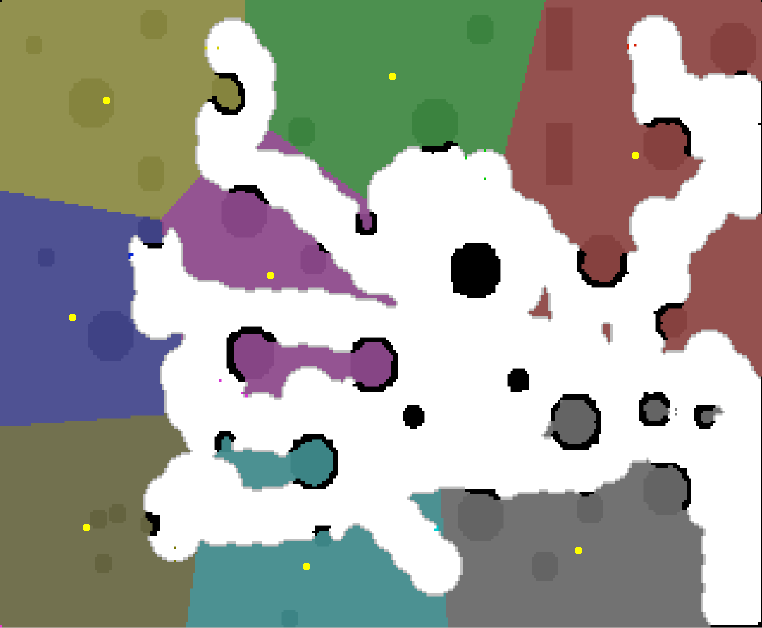
\includegraphics[width=5.5cm]{imagenes/coordGrillCM.png}
  \caption[Segmentación propuesta en \cite{Solanas2004}.]{Segmentación propuesta en \cite{Solanas2004}. En blanco se indica el espacio libre, con negro el espacio ocupado, y con colores se indica el espacio desconocido, donde cada color indica un segmento diferente dentro de los cuales se indica con tonalidades más oscuras los obstáculos todavía no explorados y con amarillo su centro de masa. Extraída de \cite{wu2007voronoi}.}\label{fig:ejemploCoodGrill}
\end{figure} 

Cada robot esta asignado al segmento cuyo centro de masa sea más cercano según la distancia euclidiana. El segmento asignado al robot $R_i$ se identifica como $\zeta_i$.
Los objetivos de exploración nuevamente serán las fronteras, la frontera $F_j$ que se asigna al robot $R_i$ es la que minimiza el $costo_{ij}$ definido en \eqref{ec:costsolanas} donde $\Delta$ es una constante que representa la distancia maxima entre dos puntos del mapa (longitud de la diagonal del mapa) $||\ ||_2$ es norma euclídea, $d$ es la distancia del camino no ocupado más corto entre dos celdas y $o_ij$ es una penalización acumulada que aumenta cuando $F_j$ esta en el rango de sensado de algún robot.

\begin{equation}\label{ec:costsolanas}
costo_{ij} = 
\begin{dcases}
  \Delta + || F_j - C_i ||_2 + o_{ij} & F_j \notin \zeta_i \\
  d(F_j, C_i) + o_{ij}                & F_j \in    \zeta_i
\end{dcases}
\end{equation}

Dado un robot $R_i$ la función de costo, a partir del valor $\Delta$, penaliza fuertemente a los objetivos que no pertenecen al segmento $\zeta_i$ asignado a $R_i$, por lo tanto los objetivos pertenecientes al segmento asignado al robot tendrán prioridad frente a los pertenecen a otro segmento, asegurando que los robots se mantendrán explorado sus segmentos asignados. Los objetivos pertenecientes a otros segmentos son considerados para permitir que un robot pueda continuar tomando objetivos aunque su segmento no tenga ningún objetivo restante. La penalización $o_ij$ evita el el solapamiento del los rangos de sensado de los robots, evitando así el trabajo redundante.\medbreak

Otro método es el que se describe en \cite{Lopez-Perez2018}, en este caso la segmentación consiste en asignar cada punto del espacio desconocido a el robot más cercano de la flota, por lo tanto el entorno se particiona en tantos segmentos $S_i$ como robots $R_i$ componen la flota de exploración. La definición exacta de los segmentos se encuentra en \eqref{ec:segmentsLopez} donde $U_i \subset M_i$ son los puntos desconocidos del espacio, $C_i$ es la posición del robot $R_i$ y la distancia $d$ se define de la misma manera que la distancia homónima del método anterior.
\begin{equation}\label{ec:segmentsLopez}
  S_i=\{c_j:d_g(C_i,c_j)\leq d(V_i(k),c_j) \forall i \neq k , c_j \in U_i\}
\end{equation}


Un ejemplo de esta segmentación se muestra en la figura \ref{fig:ejemploCoordCenter} para un entorno completamente desconocido, donde se puede visualizar las posiciones de los robots y con colores se indican los distintos segmentos. Notar que por la definición de segmento cada robot $R_i$ se encuentra dentro del segmento $S_i$ que fue definido a partir de su ubicación $C_i$. %Otra cosa a notar sobre esta técnica de segmentacion es que en este caso, donde todo el espacio es desconocido, los segmentos se corresponden directamente a las regiones de un diagrama de Voronoi generado con las posiciones de los robots como generadores y para los casos en donde el espacio no es completamente desconocido se deberá excluir los puntos conocidos de las regiones de Voronoi para obtener la segmentacion propuesta.

\begin{figure}[H]
  \center
  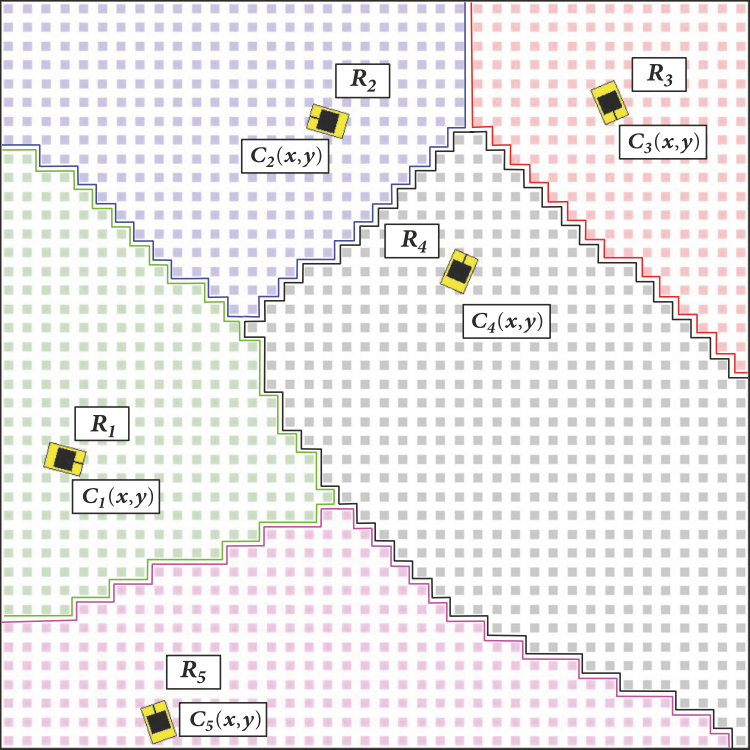
\includegraphics[width=5.5cm]{imagenes/centerCoord.png}
  \caption[Segmentación propuesta en \cite{Lopez-Perez2018}]{Segmentación propuesta en \cite{Lopez-Perez2018}, extraído de la misma fuente.}\label{fig:ejemploCoordCenter}
\end{figure} 

Una vez calculados, cada segmento $S_i$ es asignado al robot $R_i$. En este método todo punto que perteneciente a algún segmento sera un posible objetivo de exploración, por lo que en este caso sera una excepción a la norma y los objetivos no serán las fronteras sino que será todo el espacio desconocido. Los robots solo pueden ser enviados a objetivos perecientes su segmento asignado, siendo el objetivo asignado el que alcanza el menor valor para la función de peso $f_p$ que se encuera definida en \eqref{ec:weightLopez}.
\begin{equation}\label{ec:weightLopez}
  f_p(c_j) = k_d.d(C_i,c_j) + k_a.\phi_i(c_j)
\end{equation}
Donde $k_d$ y $k_a$ son dos constantes positivas que determinan el peso de cada sumando de la ecuación, la distancia $d$ es la definida en el método anterior, $\phi_i(c_j)$ es el angulo que queda definido entre la orientación del robot y el vector con origen en la posiciones del robot $C_i$, y fin en el centro de celda $c_j$. 

% \section{ Trabajos relacionados }
% A lo largo de esta sección se describen diferentes acercamientos para solucionar el problema de exploración multirobot. El primero es el presentado en \cite{amorin2019novel} en el cual se define un criterio para detener la exploracion multirobot basado en el concepto de ganacia de información. El siguiente, articulo \cite{wu2007voronoi} en el cual se 

%\subsection{Criterio de parada}
%Uno de los aspectos no mencionados hasta el momento sobre el problema de exploración es el denominado criterio de parada según el cual se determina cuando la exploración se considera finalizada. 
%Una de los criterios de parada tomados usualmente es de detener la exploración cuando el mapa construido alcanza cierto un porcentaje de cubrimiento del entorno, por ejemplo 99\% \cite{Yan2015}. Esta es usualmente utilizada para evaluaciones de rendimiento donde el entorno explorado es conocido, pero no suele ser útil en práctica, ya que para utilizarse se requiere tener conocimiento previo de las dimensiones del entorno a explorar, de lo contrario es imposible saber el porcentaje de cubrimiento.

%Otro posible criterio es el de explorar el entorno hasta que no quede ninguna posibilidad de obtener nueva información de el, osea que no exista ningún espacio desconocido que sea accesible. La desventaja de este criterio es que se fuerza a una exploration exhaustiva del entorno, lo cual puede ser indeseable por cuestiones de costos, tanto temporales, como de recursos como la energía de los robots, o su desgaste.

%En \cite{amorin2019novel} se propone un criterio de parada que carece de la necesidad de conocer las dimensiones del entorno de antemano, haciendo factible su uso en la práctica y que a su vez evita una exploración exhaustiva. El criterio se basa en el concepto de ganancia de información que hace referencia a la cantidad de información que el robot agrega al mapa construido al completar un objetivo de exploración. 

%Para experimentar y describir con detalle al criterio de parada este se define integrado a una solución en particular del problema de exploración multirobot, los aspectos de dicha solución se describen a continuación con el propósito de explicar el criterio de parada, pero también por su relevancia como ejemplo de una posible solución al problema de exploración multirobot.

%El mapa es representado como una grilla de ocupación, en este contexto la ganancia de información hace referencia a las celdas del mapa cuyo contenido es determinado luego de que un objetivo es completado. 

%La flota se compone de $N$ robots móviles circulares rígidos con capacidad para percibir toda la circunferencia alrededor con un radio $r$. Existe una estación central encargada de la tarea de reconocimiento de objetivos y asignación de los mismos. Los robots serán quienes recopilen la información del entorno y la central la encargada de crear un mapa global a partir de esta. Se consideran comunicaciones ideales, suponiendo que los robots no tienen restricciones de comunicación (por ejemplo, sin errores ni pérdidas con ancho de banda y alcance ilimitados). %Cabe aclarar que las comunicaciones inalámbricas son importantes en el contexto de exploración multi-robot.

%Para determinar los potenciales objetivos de exploración se utiliza el concepto de fronteras, que aplicado a una grilla de ocupación se asocia a las denominadas celdas fronteras son las celdas consideradas como libres y a su vez adyacentes a celdas desconocidas. Sin embargo, se argumenta que tratar todas las celdas frontera como tareas de exploración diferentes podría ser computacionalmente prohibitivo. Por lo tanto, para reducir el costo computacional, se intenta reducir los objetivos de exploración a las celdas frontera mas representativas. Para determinar que celdas frontera serán las mas representativas, primero, las fronteras se dividen en conjuntos disjuntos $F_i$. Luego, las fronteras mas representativas de cada conjunto $F_i$ se obtienen agrupando las celdas fronteras con el algoritmo k-means con $k=\frac{|F_i|}{2r}$ donde $r$ es el radio de sensado del robots. Este proceso busca reducir los objetivos de exploración de forma de que cada frontera sea perceptible desde al menos uno de los objetivos y a su vez minimizar las celdas frontera que pueden ser percibidas desde mas de un objetivo. La figura \ref{fig:ejemploFrontSig} contiene un ejemplo de las distintas partes del proceso de extracción de fronteras significativas con $r=6.l$ siendo $l$ el largo de un lado de celda.
%\begin{figure}[H]
%  \centering
%  \subfloat[Se identifican las celdas frotneras,  marcadas con amarillo.]{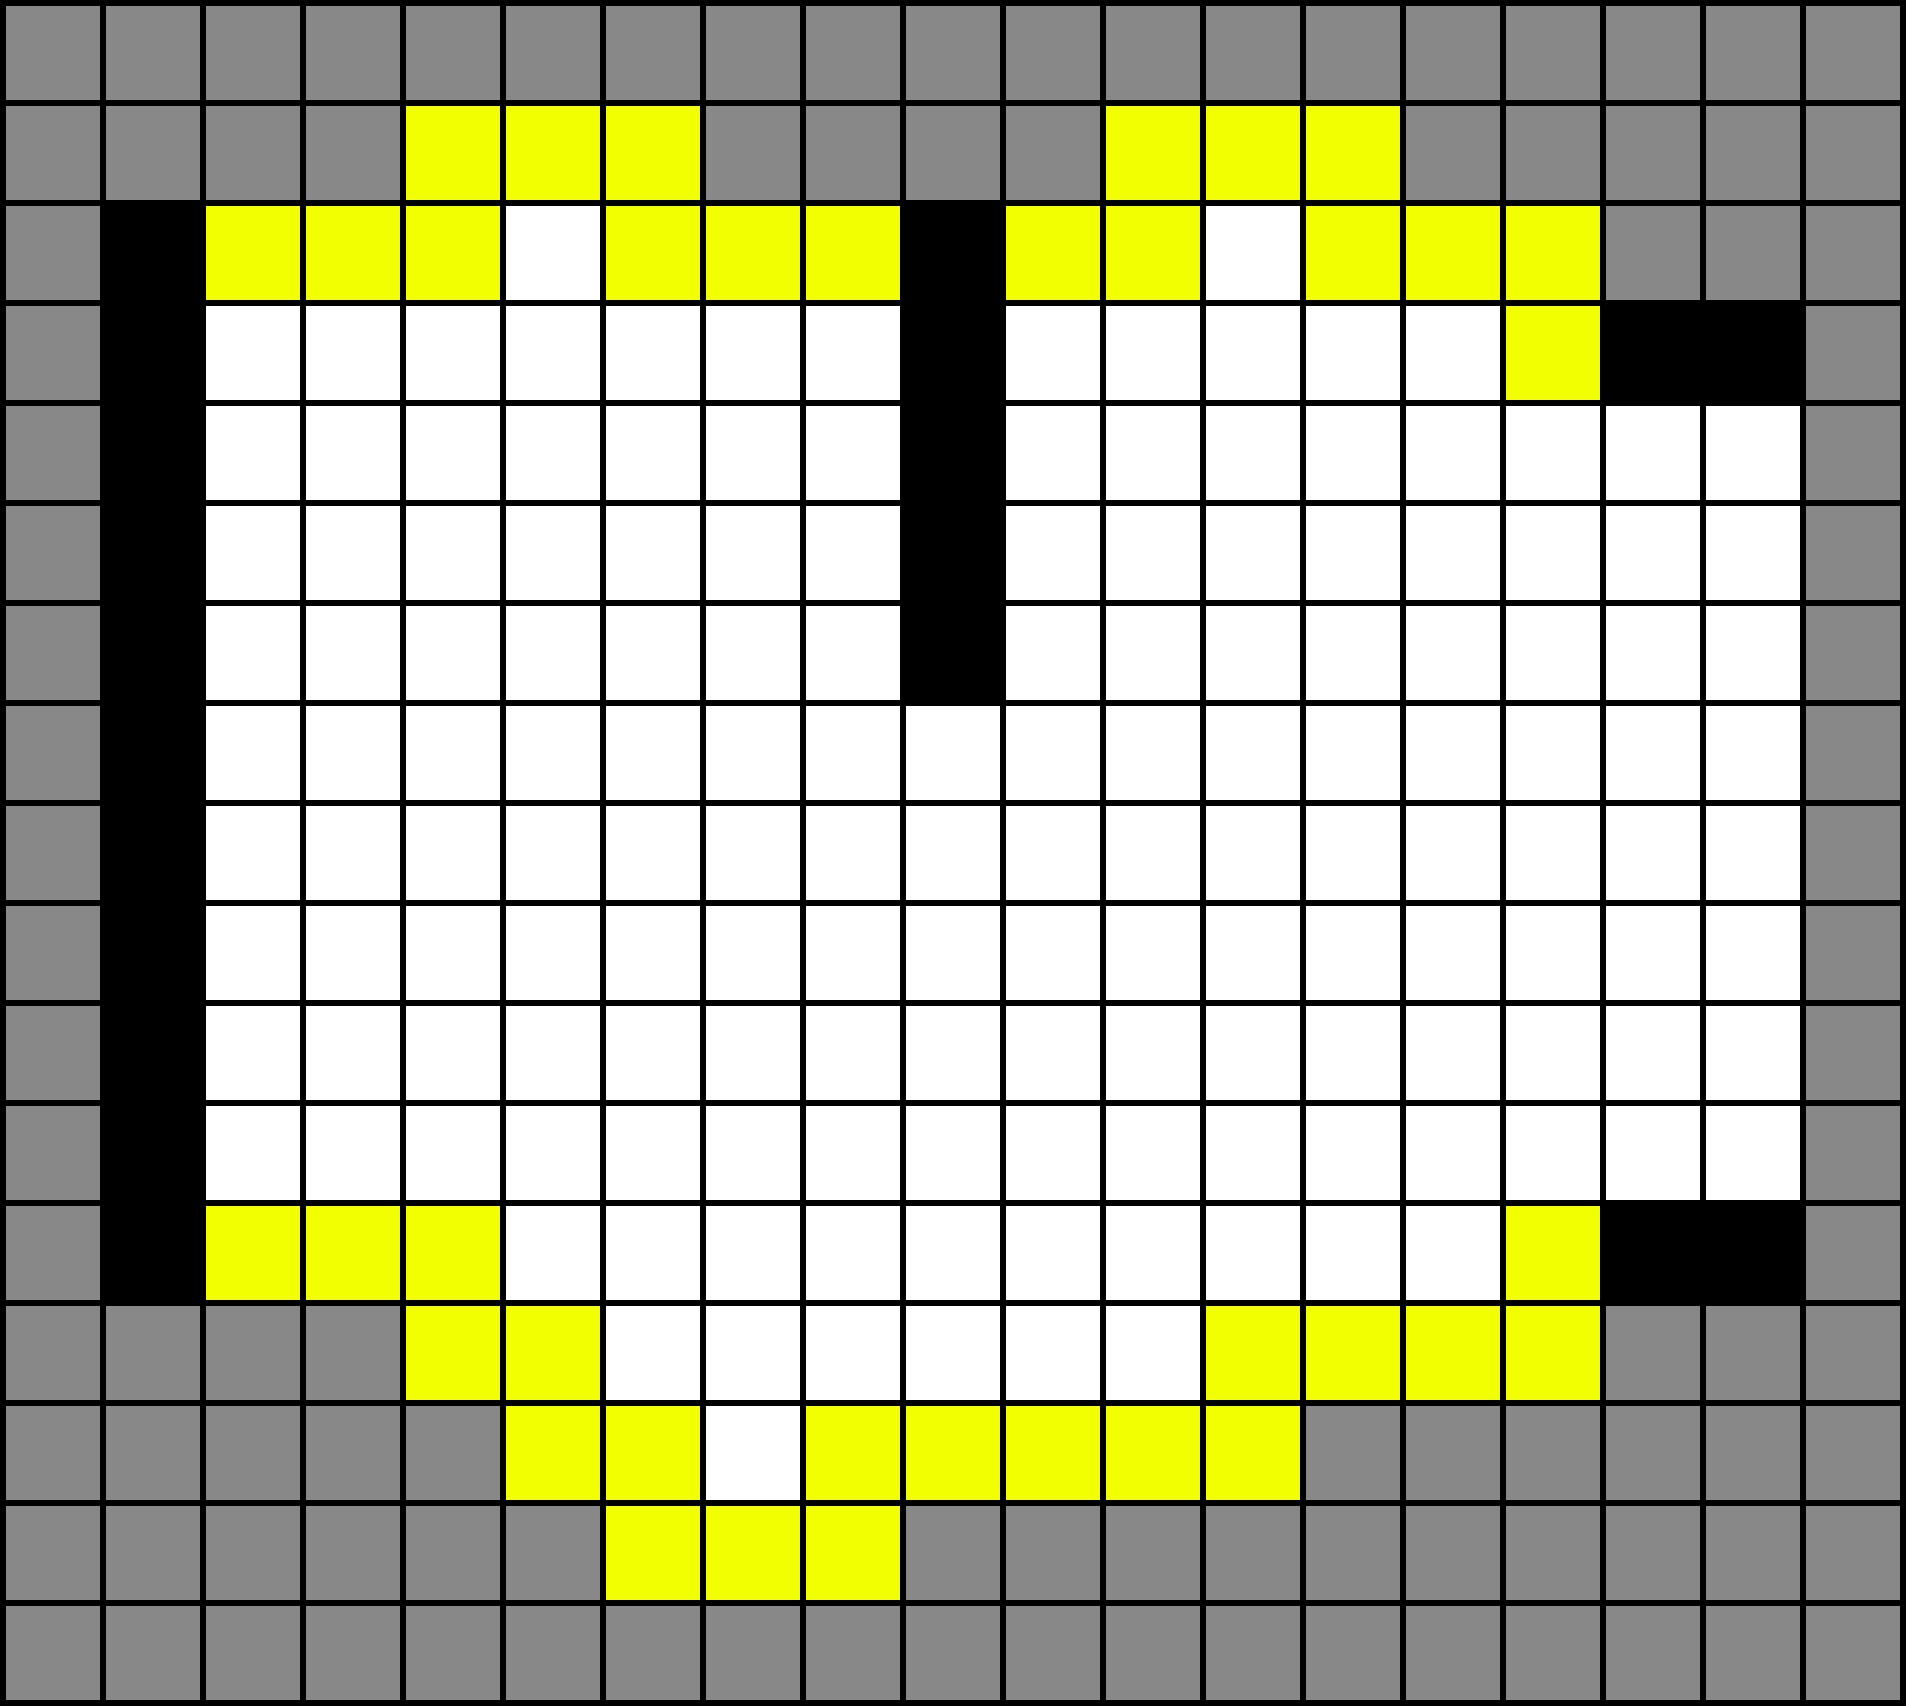
\includegraphics[clip=true, width=0.29\linewidth]{imagenes/fronterasSig/a.png}}
%  \qquad
%  \subfloat[Se Determinan los conjuntos de fornteras disjuntos $F_i$, cada color distinto representa un $i$ distinto.]{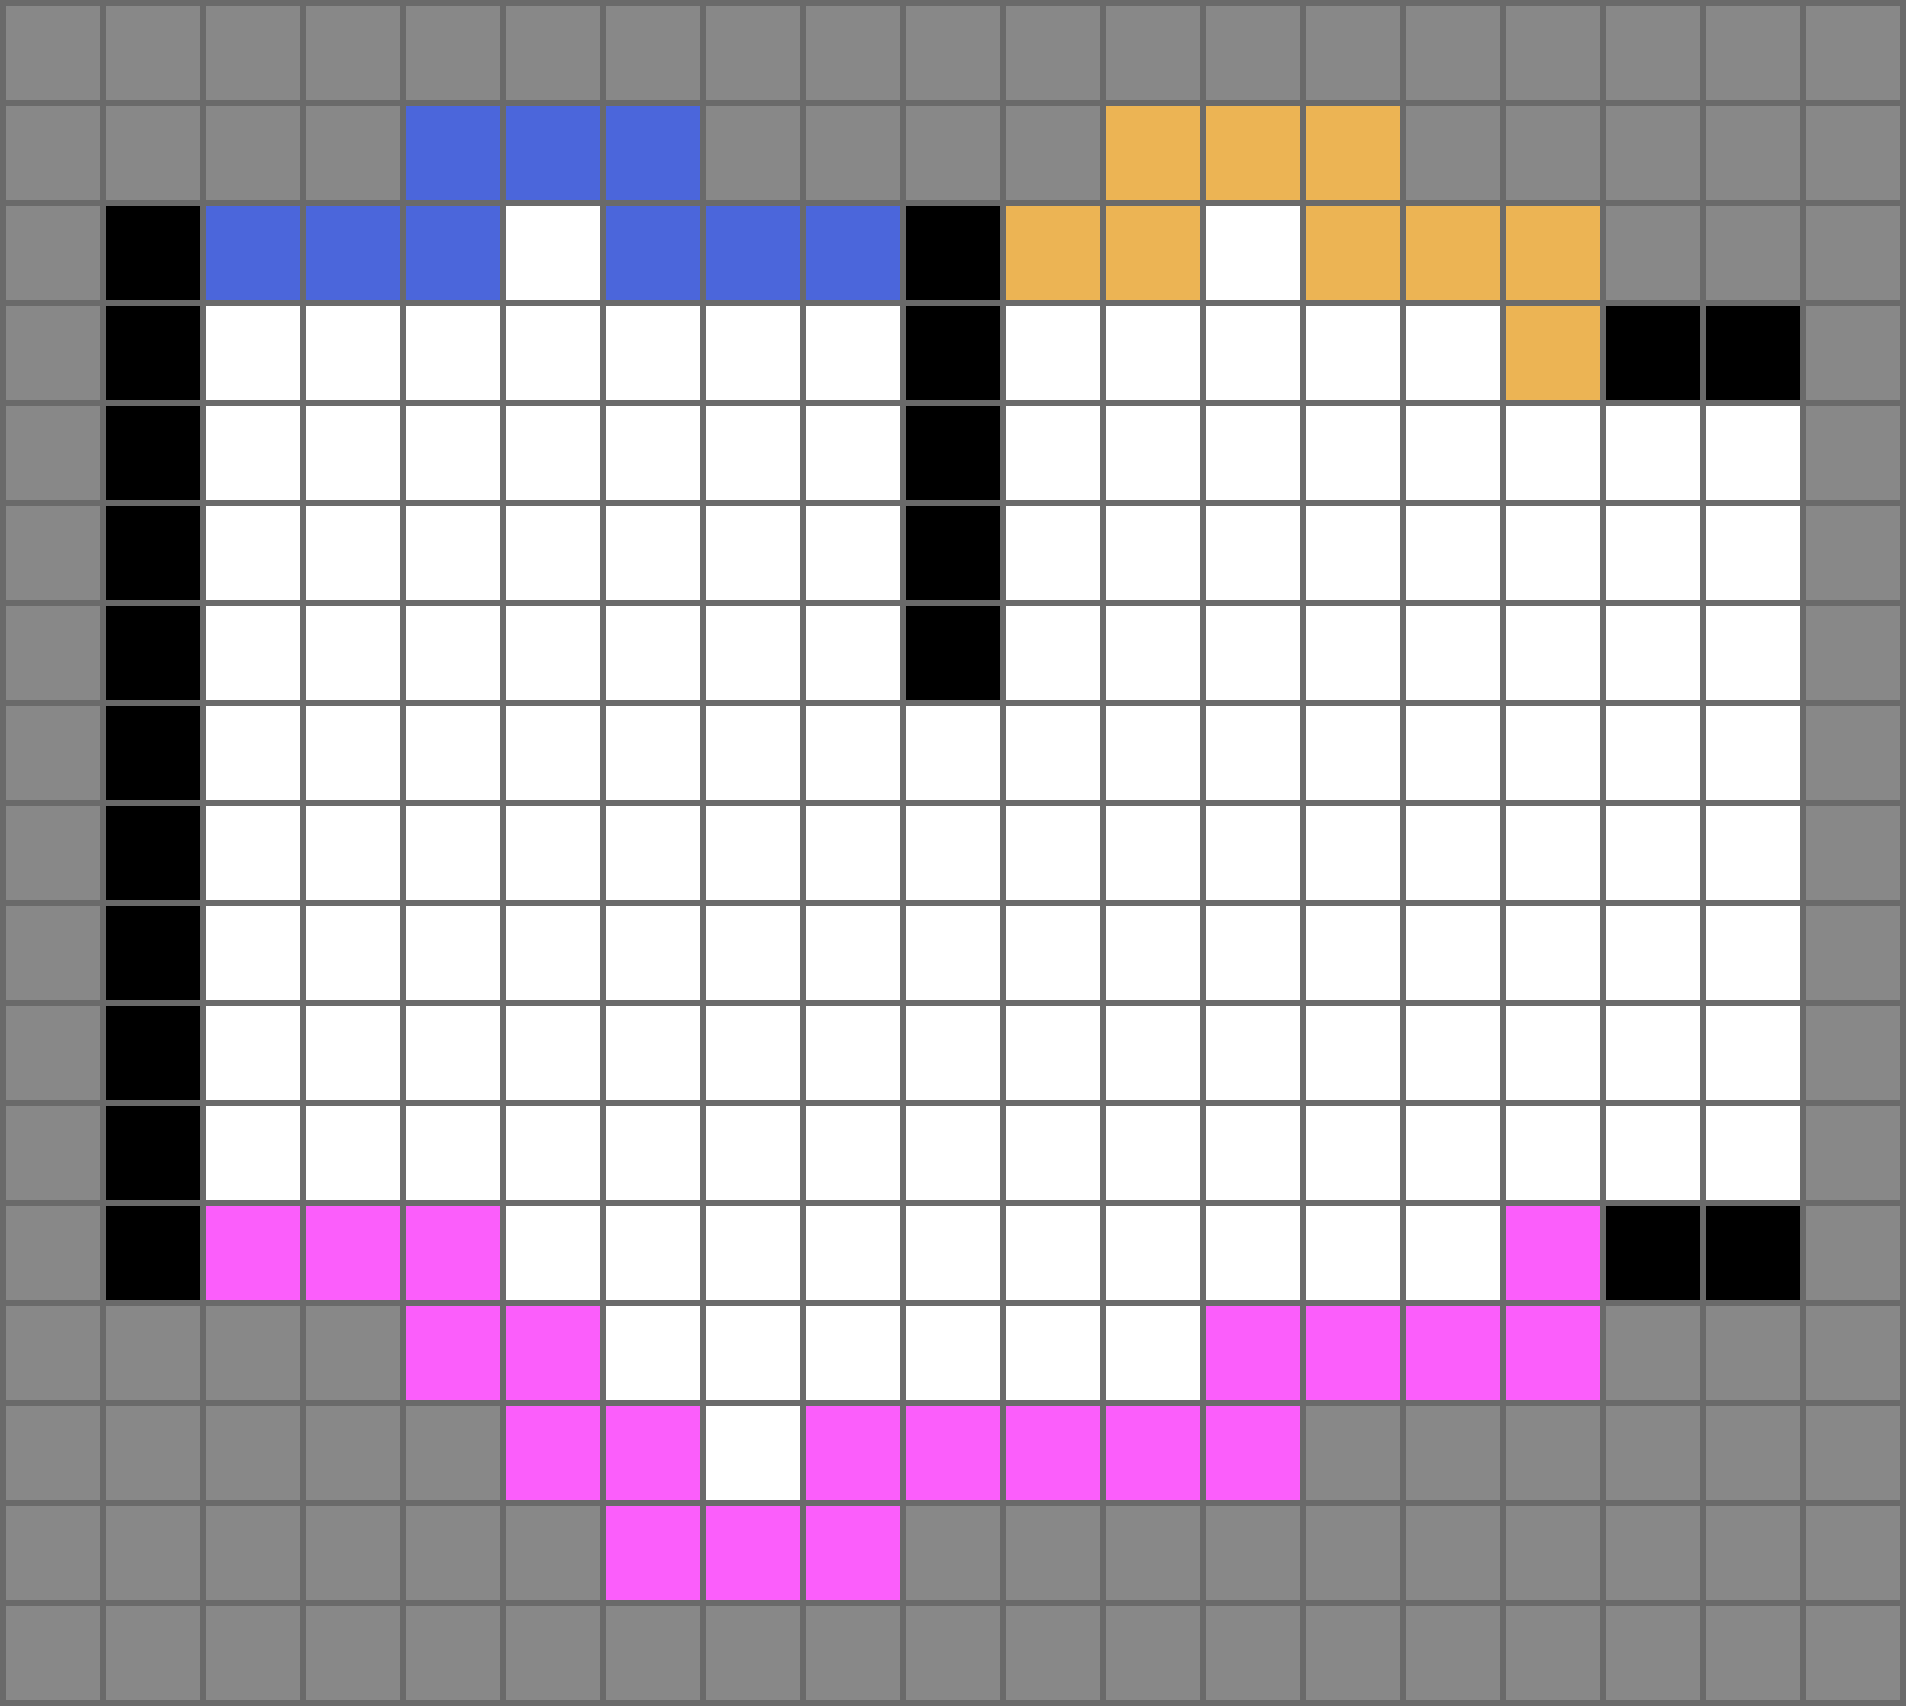
\includegraphics[clip=true, width=0.29\linewidth]{imagenes/fronterasSig/b.png}}
%  \qquad
%  \subfloat[Se obtienen las celdas frontera significativas de cada $F_i$ indicados con verde.]{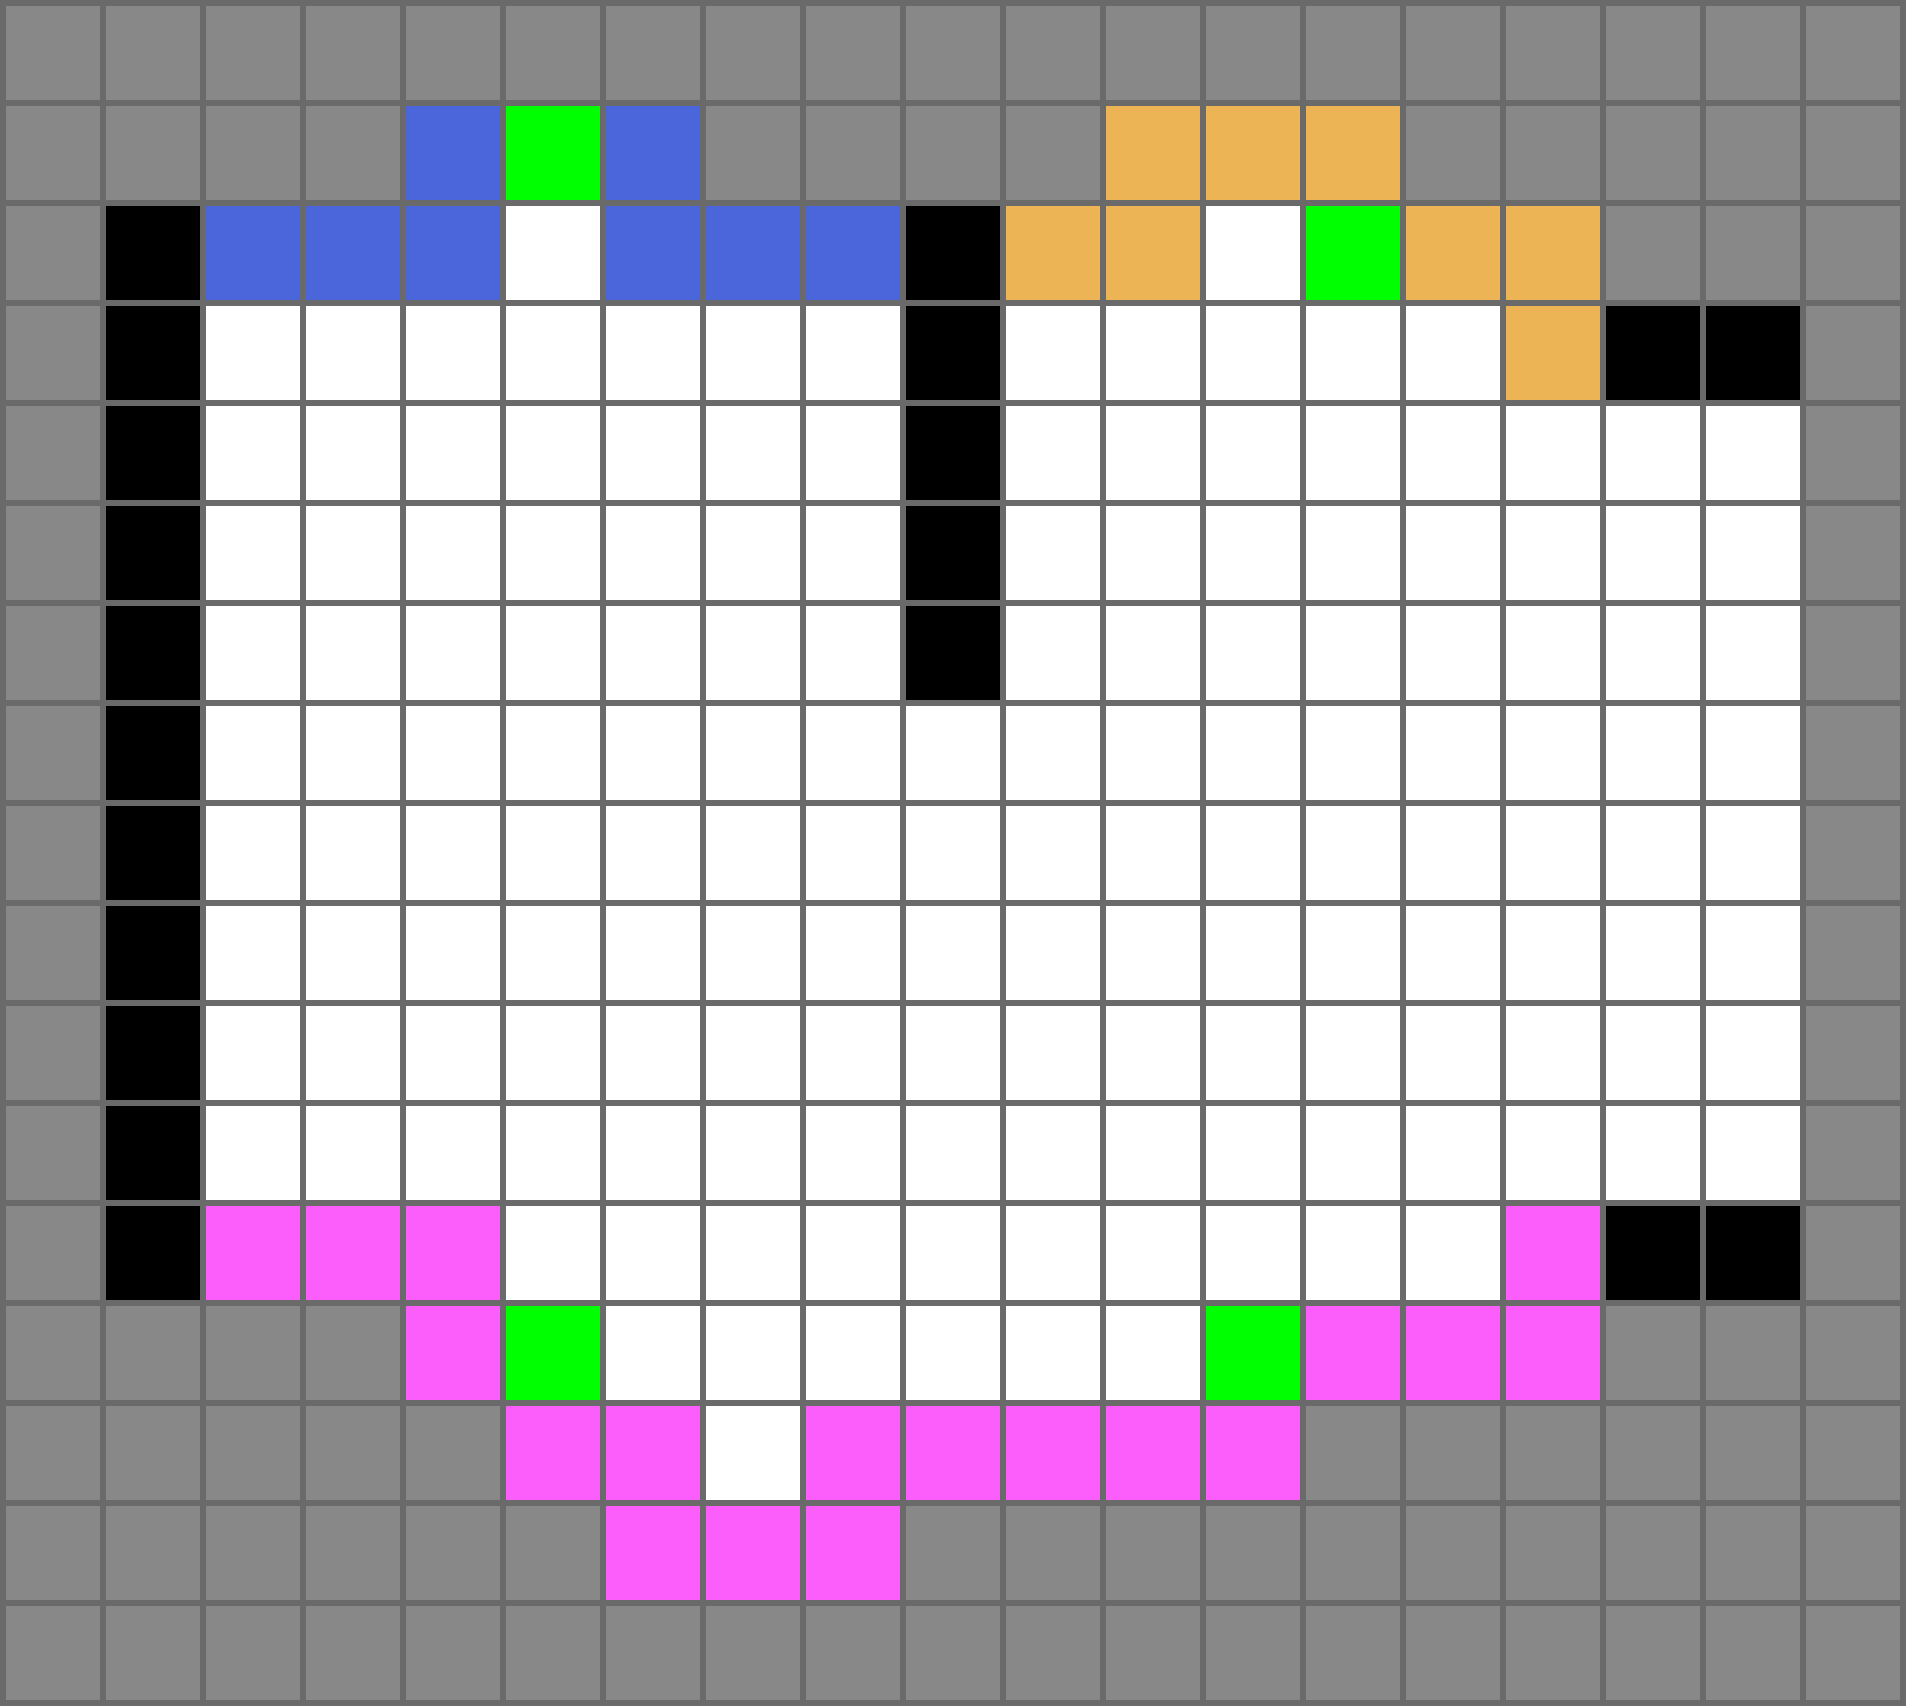
\includegraphics[clip=true, width=0.29\linewidth]{imagenes/fronterasSig/c.png}}

%  \caption[Proceso de extracción de fronteras representativas.]{Proceso de extracción de fronteras representativas. Cada figura corresponde a una etapa distinta para un mismo entorno parcialmente explorado, representado con una grilla, donde las celdas blancas son libres, las negras ocupadas, y para las grises se desconoce su estado. Extraído de \cite{Amorin2019}.}\label{fig:ejemploFrontSig}
%\end{figure}

%La asignación de objetivos de exploración se resuelve organizando una subasta entre robots, con la estación central como mediadora, es decir, encargada de dar inicio a la subasta, recibir las ofertas de los robots, determinar los resultados de la subasta e informárselos a los robots. A continuación se detallan las etapas de una subasta.

%Cuando un robot completa un objetivo de exploración (alcanza la celda frontera significativa asignada) este envía una notificación a la estación central que indica que se debe iniciar una subasta. Para dar comienzo a la subasta la estación central notifica a todos los robots sin objetivos, los cuales durante un corto período de tiempo, pueden enviar una oferta a la misma. Cada oferta consiste en una lista de pares objetivo-utilidad, donde la utilidad de un objetivo $c$ es igual a $\frac{\overline{\mli{IG}}_c}{\mli{PC}_c}$ donde $\overline{\mli{IG}}_c$ es una estimación de ganancia de información al alcanzar $c$ que se explicara más adelante y $\mli{PC}_c$ es el costo asociado a la ruta necesaria para llegar a $c$, es decir su distancia. Finalmente la central, a partir de las ofertas de todos los postores, resuelve la subasta de forma voraz, para luego notificar a cada robot su tarea asignada.

%% Dada la falta de conocimiento sobre el entorno, la mejor opción para los robots es visitar los lugares donde la ganancia de información puede ser potencialmente mayor, sin dejar de considerar el esfuerzo necesario llegar al objetivo, por lo tanto, los robots priorizarán las tareas por el coeficiente entre la ganancia de información esperada y el esfuerzo esperado necesario para completar la tarea.

%La ganancia de información estimada que es utilizada en el calculo de la utilidad y en el criterio de parada que se presentara a continuación, se calcula según \eqref{ec:infGain}. 
%%varios conceptos.  Para cada celda $c$ de la grilla de ocupacion las coordenadas $(x_c,y_c)$ son las correspondientes al centro de la celda $c$.
%\begin{equation}\label{ec:infGain}
%  \overline{\mli{IG}}_c = \overline{\mli{IG}}_{(x_c,y_c)} = |{c_i}|
%\end{equation}
%Donde toda celda $c_i$ cumple con:
%\begin{enumerate}[label=(\roman*)]
%  \item $c_i$ es una celda desconocida.
%  \item $c_i$ se puede percibir desde $c$:
%  \begin{itemize}
%    \item $c_i$ esta en rango del sensor desde $c$: $\sqrt{(x_c - x_{c_i})^2 + (y_c - y_{c_i})^2}\leq r$
%    \item No existe celda $c_o$ ocupada que obstruya a $c_i$ desde $c$:\\
%      $\nexists\ c_o \ ocupada \ \land \ \frac{ |(\frac{y_{c_o}-y_c}{x_{c_o}-x_c})(x_{c_i}-x_c) - y_{c_i} - y_{c}| }{\sqrt{(\frac{y_{c_o}-y_c}{x_{c_o}-x_c})+1}}\leq \delta $
%  \end{itemize}
%\end{enumerate}

%Siendo el valor $\delta$ igual a la mitad de longitud diagonal de una celda, por ser este la maxima distancia que puede existir entre una celda ocupada $c_o$ y el segmento de recta definido entre $c$ y $c_i$ sin que $c_o$ obstruya a $c_i$ desde $c$. En la figura \ref{fig:ejemploOclusionAm} se muestra un ejemplo de celdas que cumplen con las condiciones antes mencionadas y celdas que las cumplen, haciendo énfasis en dos celdas particulares una obstruida y otra no obstruida.

%\begin{figure}[H]
%  \centering
%  \subfloat[La celda con sus centro indicado en azul se puede precibir, esta dentro del rango del sensor y no existe un obstaculo que la obstruya.]{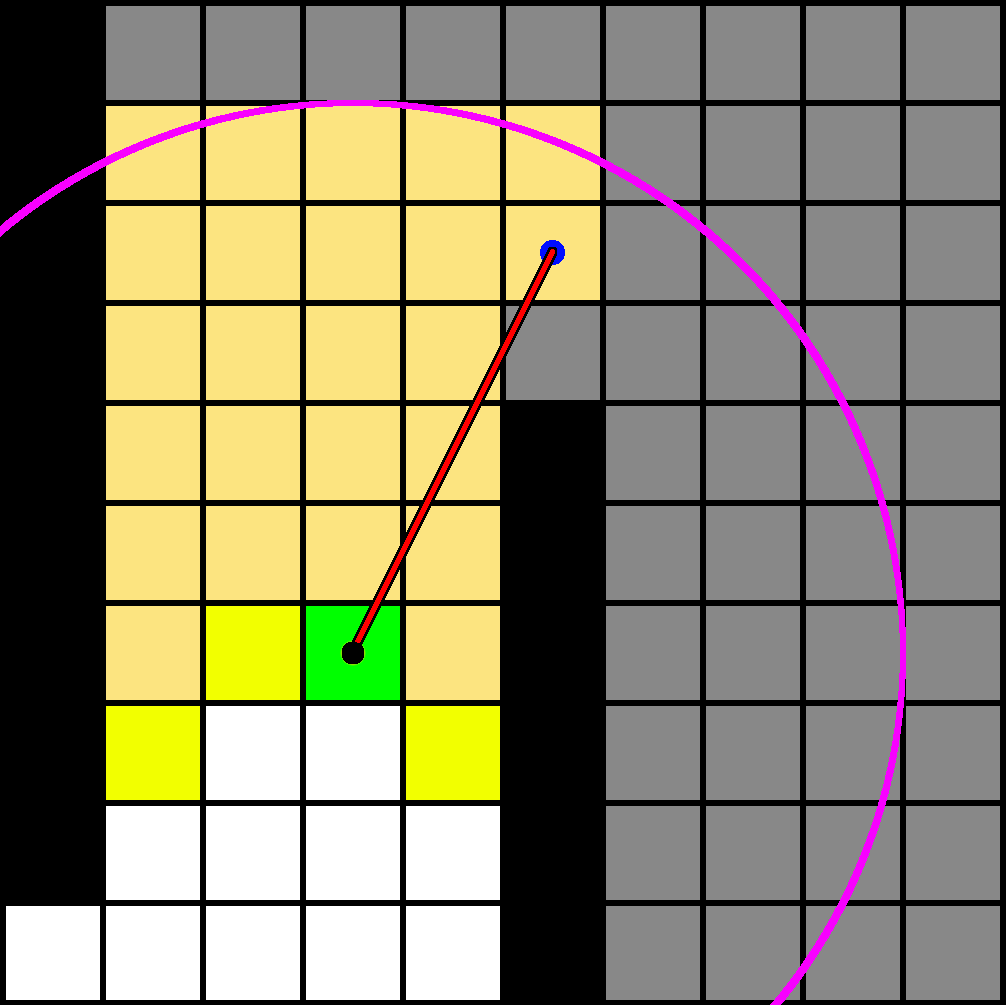
\includegraphics[clip=true, width=0.47\linewidth]{imagenes/oclusion/a.png}}
%  \qquad
%  \subfloat[La celda con su centro indicado en azul \textbf{no} se puede precibir, esta dentro del rango del sensor pero existe un obstaculo que la obstruye.]{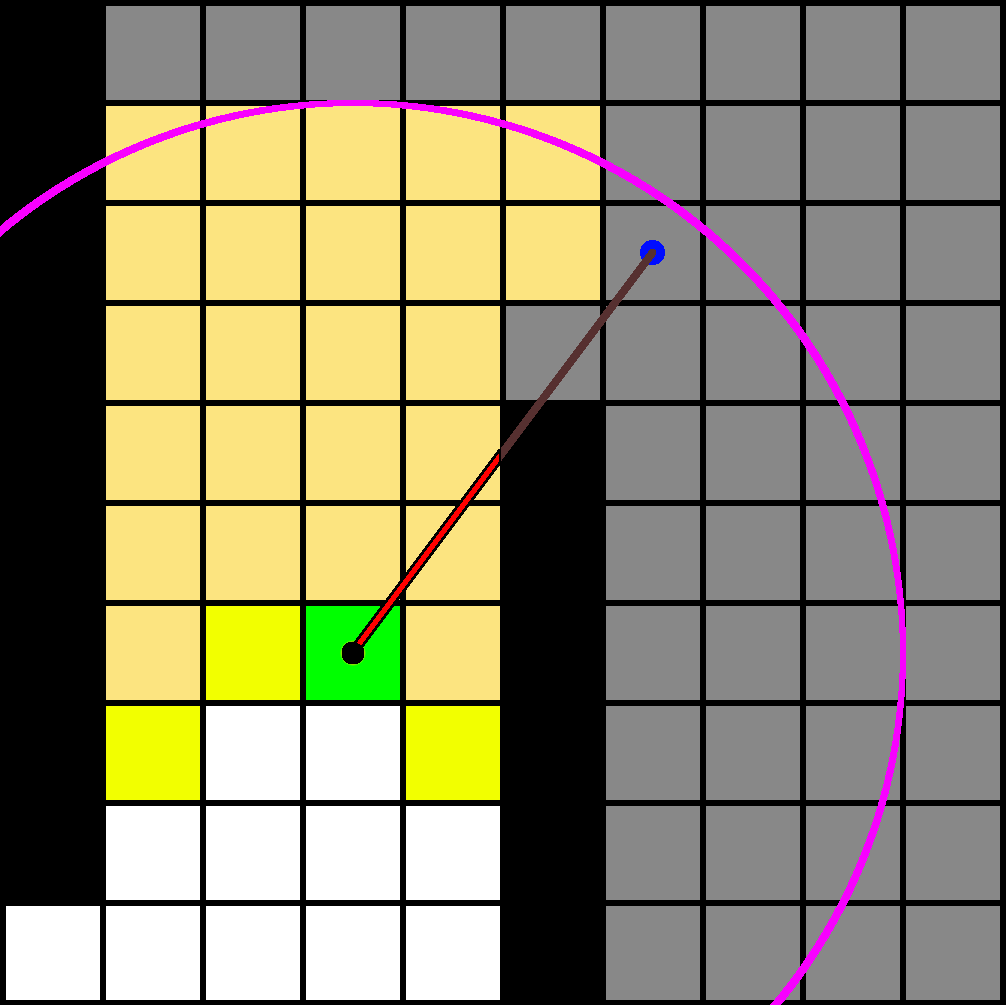
\includegraphics[clip=true, width=0.47\linewidth]{imagenes/oclusion/b.png}}

%  \caption[Condiciones que debe cumplir una celda para contabilizar en el calculo de la ganancia de información.]{Condiciones que debe cumplir una celda para contabilizar en el calculo de la ganancia de información. Lo representado por las celdas blancas, grises, negras, verdes y amarillas coincide con lo que estas representan en la figura \ref{fig:ejemploFrontSig}. Las condiciones se comprueban tomando la celda cuyo centro se marca con un punto negro como la celda $c$ y las celdas que cumplen con las condiciones se colorean con naranja. Extraído de \cite{Amorin2019}.}\label{fig:ejemploOclusionAm}
%\end{figure}



% % esto mejora sus habilidades para predecirlo de forma continua hasta que sus habilidades de predicción serán lo suficientemente buenas
%El criterio de parada propuesto en el articulo, se basa en la idea de que durante la exploración los robots obtienen conocimiento sobre el entorno, y que llegado un punto su conocimiento sobre el entorno sera lo suficientemente bueno como para estimar el estado de las zonas desconocidas del mapa de forma precisa.

%Teniendo en cuenta que una suposición básica es que la flota explora entornos limitados, las hipótesis necesarias para que el criterio de parada propuesto sea valido son dos. La primera es que existe un momento a partir del cual la estimación de la ganancia de información se puede hacer con precisión (es decir, el error cometido por el estimador tiende a cero). Y la segunda es que dicho momento puede determinarse en línea mediante robots que calculan su propio error en sus estimaciones de ganancia de información. 

%El criterio de parada consiste en finalizar la exploración cuando todos los robots, de forma independiente, determinan concluir su participación en la exploración. El criterio que un robot individual usa para determinar cuando debe dejar de explorar, es el de tener $\eta$ predicciones acertadas. Dado un umbral de tolerancia $\chi$ una una predicción es acertada cuando, al completar objetivo $c$ la diferencia entre la estimación de ganancia de información $\overline{\mli{IG}}_c$ y la ganancia de información real $\mli{IG}_c$ es menor a $\chi$ \eqref{ec:sthit}. 
%\begin{equation}\label{ec:sthit}
%  |\overline{\mli{IG}}_c - \mli{IG}_c| \leq \chi
%\end{equation}
%La idea subyacente de este criterio es al experimentar $\eta$ predicciones acertadas un robot tiene la suficiente información sobre el entorno como para poder estimar la porción inexplorada con precisión, y por lo tanto podrá detenerse.

%%%%%%%
% Desde acá proyecto de grado redactado
%%%%%%%

% \subsection[Distributed Multi-robot Exploration Based on Scene Partitioning and Frontier Selection]{Distributed Multi-robot Exploration Based on\\ Scene Partitioning and Frontier Selection}
% \subsection{Exploración multirobot distribuida} \todo{esta sección iría arriba, luego de exploración multirobot pero hay que ver bien qué se espera. es decir, el tema es vasto pero se nombra sólo una ref. tendrá algo de especial. pensaría bien cuál es el objetivo y vería}
% % Al considerase una solución para el problema de exploración hay dos aspectos centrales a resolver, identificar posibles objetivos de exploración y como priorizar estos objetivos de forma de priorizar los mas relevantes.

% En \cite{Lopez-Perez2018} se propone una solución completamente distribuida al problema de exploración multirobot. Este tipo de resolución implica descentralización, lo que aumenta tanto la robustez del sistema como su autonomía en tanto solo se requiere del equipo robótico para explorar el entorno, sin depender de una entidad central para coordinar ningún aspecto de la solución. %, que al igual que otras ya comentadas partición el entorno aunque en este caso dicha 

% \subsubsection{Formulación del problema}
% La variante del problema de exploración multi-robot tratada en este articulo es la de explorar un entorno desconocido $W\in R^2$ utilizando un conjunto de robots $R={R_1,R_2,...,R_n}$. Se utiliza una grill  de ocupación, por lo que el entorno se descompone en un conjunto de celdas $C={c_1,c_2,...,c_n}$. Cada robot $R_i$ posee: 
% \begin{enumerate}
%   \item Un mapa $M_i \in CxL$ donde $L$ son las diferentes estados en los que puede estar una celda. 
%   \item Una posición inicial $q_{init}^{i}\in R^2 \times [-\pi,\pi]$. 
%   \item Un sensor $S_i$ para explorar el entorno desconocido.
% \end{enumerate}

% Adicionalmente se asume que existe siempre un cuadro delimitador de $W$ que puede ser establecido, aunque sea de forma aproximada, antes de que la exploración comience, comunicación perfecta (sin perdida y de rango infinito) y que cada robot tiene acceso a su posición respecto a un marco de referencia común.

% \subsubsection{Descripción del sistema}
% El sistema tiene un diseño modular, este consta de 4 módulos que se encuentran replicados en cada robot, el modulo de distribución de información, el modulo de asignación de zonas, el modulo de adquisición de información y el modulo de exploración. Estos se describen en las siguientes secciones. 

% \paragraph{Modulo de distribución de información}
% Este modulo se encarga de distribuir a los demás robots la posición del robot al que pretence, las ubicaciones que conoce de los demás robots y su mapa $M_i$. 

% \paragraph{Modulo de asignación de zonas }
% El entorno es segmentado en zonas y la exploración cada una de estas es asignada a un robot. El modulo de asignación de zonas es el responsable de realizar la segmentación en zonas y su posterior asignación a los robots. La segmentación genera tantas zonas $E_i$ como robots $R_i$ que $E_i$ se define en \eqref{ec:zones} a partir de la posición $C_i$ de $R_i$. .
% \begin{equation}\label{ec:zones}
%   E_i=\{c_j:d_g(C_i,c_j)\leq d_g(V_i(k),c_j) \forall i \neq k , c_j \in U_i\}
% \end{equation}
% Donde $U_i \subset M_i$ son la celdas desconocidas del mapa asociado al robot $R_i$ y $d_g(c',c'')$ es la distancia geodésica, que indica el camino compuesto de centros de celdas mas corto entre dos celdas $c'$ y $c''$ que respecta la conectividad entre las celdas que lo componen.

% Cada zona $E_i$ es asignada al robot $R_i$ y este explorara las celdas de $E_i$ según lo determine el \hyperref[par:estar:moduloexp]{modulo de exploración}.

% \paragraph{Modulo de adquisición de información}
% El propósito de este es el de actualizar el mapa $M_i$ de el robot $R_i$ según la información obtenida por su sensor $S_i$ y su posición $C_i$.

% \paragraph{Modulo de exploración}\label{par:estar:moduloexp}
% El modulo de exploración esta compuesto por tres submódulos. 

% El primero de ellos es el submódulo de asignación de objetivos, como su nombre lo indica, este se encarga de seleccionar un objetivo de todos los pertenecientes a la zona asignada $E_i$ para asignarlo al robot $R_i$. El objetivo seleccionado $G_i$ es el que alcanza el menor valor para la función de peso $f_p$ que se computa como \eqref{ec:weight}.
% \begin{equation}\label{ec:weight}
%   f_p(c_j) = k_d.d_g(C_i,c_j) + k_a.\phi_i(c_j)
% \end{equation}
% Donde $k_d$ y $k_a$ son dos constantes positivas que determinan el peso de cada sumando, $d_g(C_i,c_j)$ hace referencia a la distancia geodésica mencionada anteriormente, $\phi_i(c_j)$ es el angulo entre la orientación del robot y el vector con origen en la posiciones del robot $C_i$, y fin en el centro de celda $c_j$. 

% Luego esta el submódulo de planificación de ruta, este se encarga de generar una ruta que le permita al robot llegar al objetivo asignado. Esto se logra a partir del algoritmo $A*$, para la ejecución de este se asume que las celdas desconocidas son libres. En el caso de encontrarse un obstáculo en la ruta planificada se replanifica ejecutando nuevamente el algoritmo $A*$ en la version mas reciente del mapa.

% El último es el submódulo de ejecución de trayectoria que se encarga de generar los comandos de actuación para seguir una ruta planeada.
\section{Simuladores}

% Introducción sobre porque simular esta bueno.

La simulación es una herramienta de gran utilidad en el contexto de la robótica
y fundamental en el desarrollo de este proyecto. 

Los simuladores robóticos modelan la realidad con el propósito de %poder
reproducir computacionalmente los aspectos de esta que son relevantes para la
robótica. Específicamente un simulador robótico debe proporcionar un modelo de
las interacciones físicas (gravedad, colisiones, iluminación, viento, entre
otros) como permitir representaciones realistas de robots incluyendo sus
sensores, actuadores y transductores.

La utilidad principal de los simuladores es que permiten realizar pruebas sin
necesidad de robots, ni de entornos reales. Esto permite validar de forma
rápida y económica soluciones a problemas complejos. Pero no es un remplazo
para  pruebas en la realidad, ya que los modelos utilizados realizan
simplificaciones que pueden causar cambios con respecto al comportamiento
real.

Actualmente existe una gran variedad de simuladores robóticos, de los cuales se consideraron
cuatro como candidatos para utilizar en el proyecto, Gazebo\footnote{\url{http://gitlab.fing.edu.uy/federico.ciuffardi/gazebo_benchmark}},
CoppeliaSim\footnote{\url{http://www.coppeliarobotics.com}} (antes conocido como V-Rep), ARGoS\footnote{\url{http://www.argos-sim.info}}
y Webots\footnote{\url{http://cyberbotics.com}}.
% Actualmente existe una gran variedad de simuladores robóticos, de los cuales se consideraron
% cuatro como candidatos para utilizar en el proyecto, Gazebo \cite{gazebo},
% CoppeliaSim \cite{coppeliasim} (antes conocido como V-Rep), ARGoS \cite{argos}
% y Webots \cite{webots}.


En las siguientes secciones se realiza un análisis comparativo de los simuladores
candidatos que concluye con la elección de uno de ellos para su uso en el
proyecto.

%Esto en primer lugar permite concentrarse en los aspectos
%más fundamentales de lo que se prueba ya que permite facilidades que en la realidad no son posibles como evitar aspectos de comunicación, 

% Las principales ventajas asociadas a la simulación se derivan del 

% tienen como propósito replicar escenarios 

% permite realizar experimentos evitando   e una alternativa que permite validar propuestas de forma


\subsection{Características}
% Presentar tabla. Describir características, basado en articulos. 

Existen varios estudios comparativos de simuladores robóticos que incluyen
alguno de los candidatos \cite{Nogueira2014, SantosPessoadeMelo2019,
ramli2015overview, Pitonakova2018}. 
%Con el propósito de conocer más acerca de cada uno y de poder determinar cual es una buena elección para el proyecto se
Se analizó dichos artículos y se estudió la información que se encuentra pública
en las páginas oficiales en busca de características consideradas de utilidad, los resultados se resumen en la  
en la tabla \ref{tab:sims}. 

\begin{table}[H]
\hbadness = 10000
\tolerance=9999
\emergencystretch=10pt
\hyphenpenalty=10000
\exhyphenpenalty=100
\begin{center}
  \begin{tabularx}{\textwidth}{|X|X|X|X|X|}


\hline
                      & Gazebo                          & CoppeliaSim                      & Webots                          & ARGoS                               \\ \hline
Multiples robots      & \cellcolor{green!25}Si          & \cellcolor{green!25}Si           & \cellcolor{green!25}Si          & \cellcolor{green!25}Si              \\ \hline
Simuladores físicos disponibles &                                                                                                                                         
  %gazebo
  \cellcolor{green!25}Bullet, ODE, Sim-body y DART  & 
  %copelia
  \cellcolor{green!25}Bullet, ODE, Vortex y Newton  &
  %webots                                           
  \cellcolor{green!25}ODE                           &
  %argos                                            
  \cellcolor{yellow!25} Propios                     \\ \hline
Integración con ROS   & \cellcolor{green!25}Si          & \cellcolor{green!25}Si           & \cellcolor{green!25}Si          & \cellcolor{red!25}Inactiva \\ \hline 
Aceleración de tiempo & \cellcolor{green!25}Si          & \cellcolor{green!25}Si           & \cellcolor{green!25}Si          & \cellcolor{green!25}Si     \\ \hline
Modo headless         & \cellcolor{green!25}Si          & \cellcolor{green!25}Si           & \cellcolor{red!25}No            & \cellcolor{green!25}Si     \\ \hline
Licencia              & \cellcolor{green!25}Apache 2.0  & \cellcolor{yellow!25}Propietaria & \cellcolor{green!25}Apache 2.0  & \cellcolor{green!25}MIT    \\ \hline
  \end{tabularx}
  \caption{Comparación entre simuladores.}
  \label{tab:sims}
\end{center}

\end{table}
% Pre conclusion segun las caracteristicas, introducir necesidad de experimentar

Todos los simuladores candidatos permiten simular varios robots simultáneamente
lo cual es esencial en el marco del proyecto. 

% \cite{ode} \cite{bullet}
Webots solo dispone de ODE \footnote{\url{http://www.ode.org}} para la simulación física,
mientras que Gazebo y CoppeliaSim disponen de varias alternativas entre las
cuales se incluyen ODE y Bullet \footnote{\url{http://pybullet.org}}. Tanto ODE como Bullet son conocidos
motores de físicas cuyas capacidades han sido estudiadas en diversos artículos
\cite{bzhikhatlov2017research,erez2015simulation,ronnau2013evaluation}.
ARGoS por su parte dispone de un simuladores 2D y 3D personalizados que según
\cite{Pitonakova2018} son mucho más simples que los utilizados por Gazebo y
CoppeliaSim. Esta simplicidad se comenta que esta asociada con capacidades
limitadas, pero también es posible que sea un factor que influye positivamente
en la eficiencia.


ROS \cite{ros} es un framework que facilita el desarrollo de aplicaciones
robóticas, utlizarlo evita \say{reinventar la rueda} y permite dedicarse
a los aspectos principales de un proyecto. 
%Otro aspecto importante es que implementar con ROS
%puede facilitar la migración de la implementación desarrollado en el
%simulador para en la realidad.
De los simuladores candidatos
todos menos ARGoS proveen de soporte oficial para ROS. Para ARGoS existe una
extension \cite{argos_bridge} que permite conectar a ROS con ARGoS que se
encuentra inactiva. %hace cinco años.
\todoremark{La introducción a ros, no se si deberia estar aca. La parte de migrar se entiende? deberia fundamentar mas? sacarla?}

%utilizando las
%facilidades estándar (por ejemplo el stack de navegación) es que el código
%desarrollado para funcionar en el simulador se migre para funcio

La posibilidad de acelerar el tiempo se encuentra presente en todos los
simuladores, lo cual es deseable para reducir el tiempo real que lleva ejecutar
una simulación, siempre y cuando el hardware que corra la simulaciones sea lo
suficientemente potente para permitirlo. 

Ejecutar en modo \emph{headless} es ejecutar sin una interfaz gráfica, esto es
útil porque permite dedicar más recursos computacionales a la simulación.
Esto se permite en todos los simuladores estudiados, menos en Webots.

Con respecto a las licencias Gazebo, Webots y ARGoS tienen licencias
libres \cite{fsf}, mientras que CoppeliaSim tiene una licencia propietaria.
Aunque la licencia de CoppeliaSim permite su uso no comercial de forma gratuita
con propósitos educacionales, es deseable el uso de alternativas libres.

En \cite{Pitonakova2018} se presenta un estudio comparativo de eficiencia entre
CoppeliaSim, Gazebo y ARGoS. El estudio se basa en experimentos que consisten
en distintas cantidades de robots (1, 5, 10 y 50) que se mueven en linea recta por un minuto
evitando obstáculos en tiempo real. Esto se repitió en dos entornos distintos
uno simple y otro complejo. Los experimentos evaluaron el rendimiento (a través
de la aceleración de tiempo) y el uso de recursos (RAM y CPU). CoppeliaSim
consistentemente presenta los peores resultados en uso de recursos y
rendimiento, considerándose inviable la ejecución de las pruebas que utilizan
50 robots. Entre ARGoS y Gazebo en términos de uso de recursos ARGoS resulta
superior en todos los casos. Con respecto al rendimiento, en casos simples
(pocos robots o entorno simple) ARGoS es mejor, mientras que Gazebo es mejor en
casos complejos (muchos robots y entorno complejo).

Dada la información presentada hasta el momento es posible descartar a ARGoS como
opción dado que su simulación se considera poco realista y por su falta de
integración con ROS. Por su licenciamiento propietario, bajo rendimiento y alta
utilización de recursos, se descarta a CoppeliaSim como posibilidad. Entre los
restantes Gazebo y Webots la información disponible dificulta tomar una
decisión. Se busco sin éxito estudios de rendimiento y/o uso de recursos sobre
Webots. Dado esto se decidió realizar un pequeño estudio comparativo propio
entre Webots y Gazebo, cuyo objetivo sea evaluar el rendimiento y usabilidad de
ambos.

\subsection{Experimentación}
% Haber introducido la necesidad de experimentar o introducirla acá.

% Quizás puedo resumir los resultados y poner el resto en un anexo, o no, ver.
\subsubsection{Método}
El experimento se basa en replicar un mismo escenario en Gazebo y Webots una
consiste en dos paredes de $20m$ paralelas que están a $10m$ una de la otra.
Entremedio de estas se ubican 3 robots diferenciales pioneer 3-DX uno alineado
con el centro de las paredes, uno a la izquierda y otro a la derecha ambos a
$5m$ del que se encuentra en el centro. En la figura \ref{fig:impsim} se
muestra el escenario de simulación implementado en los simuladores a evaluar.

\begin{figure}[H]
  \centering
  \subfloat[Gazebo.]{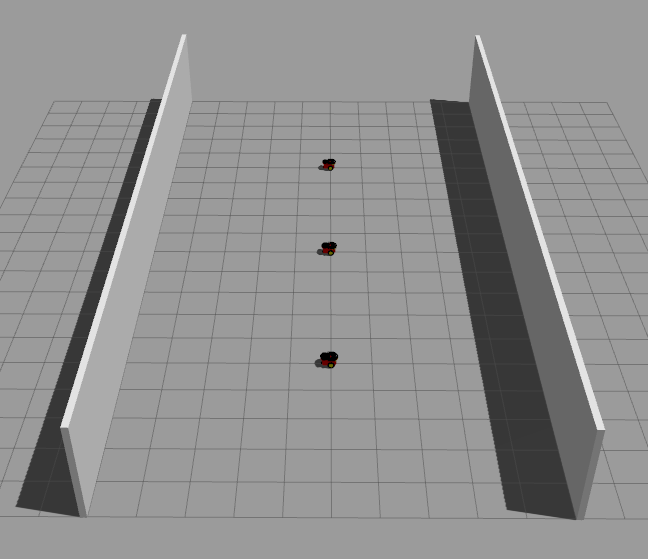
\includegraphics[clip=true, width=0.40\linewidth]{imagenes/sim/gazebo1.png}}
  \qquad
  \subfloat[Webots.]{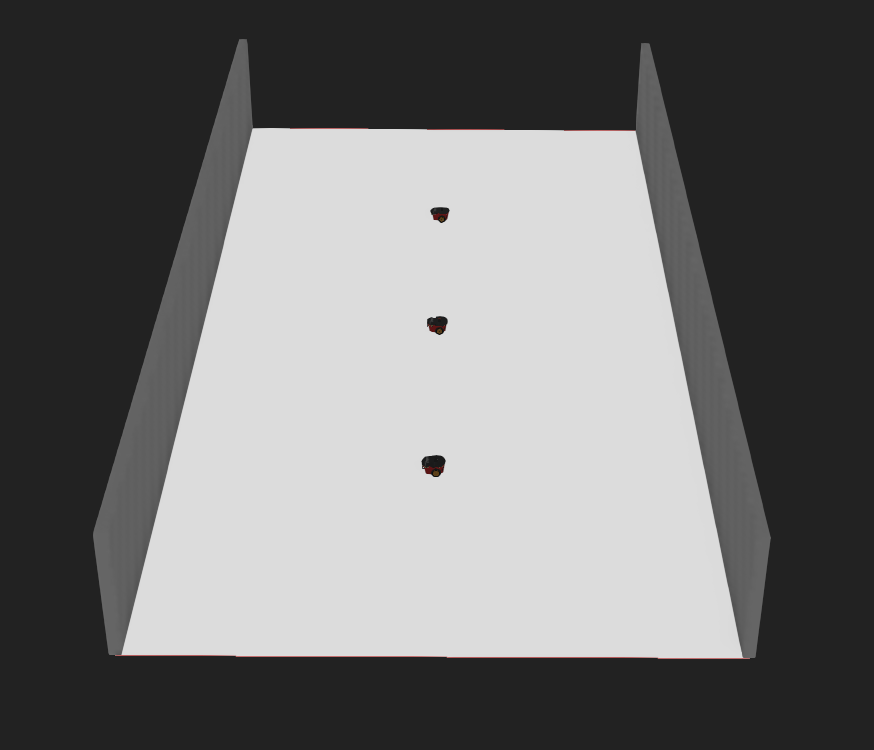
\includegraphics[clip=true, width=0.40\linewidth]{imagenes/sim/webots1.png}}
  \caption{Implementaciones del escenario de simulación.}\label{fig:impsim}
\end{figure}

Al ejecutarse la simulación los robots deben avanzar hasta una de las paredes
cuando se encuentran a un metro de esta (información obtenida usando un LiDAR)
estos cambian de dirección repitiendo el comportamiento por cinco minutos.

El proceso de replicar el escenario en cada simulador utilizando ROS será el
insumo para evaluar su usabilidad, mientras que para evaluar el rendimiento y
comportamiento se ejecutará una vez ambas simulaciones acelerando el tiempo
tanto como sea posible, siendo $R_{sim}$ (\ref{ec:R}) el indicador de
rendimiento resultado de dividir el tiempo dentro de simulación $ts$ entre el
tiempo real que tome ejecutarla $tr$. A mayor $R_{sim}$ mayor rendimiento.
\begin{equation}\label{ec:R} R_{sim} = \frac{ts}{tr} \end{equation}

El software utilizado fue Ubuntu \emph{20.04}, ROS \emph{Noetic}, Gazebo \emph{11.4.0} y Webots \emph{R2021a}. 

El hardware consiste de un procesador Intel Core i3-9100F, un procesador
gráfico GeForce GTX 660 y 16GB de memoria RAM.

\subsubsection{Resultados}
%\cite{gazebo_benchmark}
Las implementaciones del escenario de prueba en Gazebo y Webots se encuentran
disponible en linea\footnote{\url{http://gitlab.fing.edu.uy/federico.ciuffardi/gazebo_benchmark}}
\footnote{\url{http://gitlab.fing.edu.uy/federico.ciuffardi/webots_benchmark}}. 

La construcción del entorno fue similar en ambos simuladores siendo
más cómoda en Webots ya que este dispone por defecto del modelo de robot a
utilizar, por otro lado en Gazebo fue necesario usar un modelo creado por un
tercero.

En términos de integración con ROS, en Gazebo se logró sin inconvenientes,
Webots requirió más trabajo en tanto no integra facilidades para el control de
robots. Por ejemplo, Webots no soporta el uso del paquete de ROS
\emph{diff\_drive\_controller} \cite{diff_drive_controller} que simplifica el
control de movimiento de robots diferenciales, mientras que Gazebo sí.
\todowarn{Hay otros aspectos que Detecte como malos de Webots, como necesidad
  de usar servicios para activar los tópicos, en vez de que estén activos por
defecto pero me parece que es complicado de explicar en alto nivel}

Otro aspecto que complejizó la integración de ROS en Webots es que su sistema
de coordenadas por defecto (NUE) difiere del utilizado por ROS y Gazebo (ENU).
Fue posible configurar Webots para utilizar ENU pero se requirió hacer algunos
cambios como rotar los elementos  del entorno manualmente.
% - Diferentes estandares en los sistemas coordenadas entre ROS("ENU") y Webots("NUE") que aunque Webots permite cambiarlo esto solo altera las traslaciones pero no las rotaciones, por lo tanto, ademas de tener que rotar todos los objetos en el mapa, otras consideraciones pueden ser necesarias. El ejemplo que se presenteo durante el desarrollo del bechmark fue la necesidad rotar los frames de referencia de los datos un lidar para visulaizarlos correctamente en rviz.

Al ejecutar las simulaciones en Gazebo el comportamiento fue el esperado, en
Webots los robots se balanceaban notoriamente de adelante hacia atrás al
moverse, mientras que las medidas provistas por el LiDAR no se corresponden con
las ubicaciones de la pared.

Los resultados de rendimiento fueron para Webots $R_{sim}=2.20$, para Gazebo $R_{sim}=3.58$
en su modo normal y $R_{sim}=4.70$ haciendo uso del modo \emph{headless} que Webots no dispone.

\subsection{Conclusiones}

Con respecto a la usabilidad, Webots presenta la ventaja de tener
disponible el modelo deseado, pero esto queda opacado por los inconvenientes
experimentados al integrar con ROS\footnote{La version R2021b de
Webots agrega soporte para \emph{diff\_drive\_controller}}. Gazebo resulto tener una mejor usabilidad al no presentar dichos
inconvenientes.

La simulación en Gazebo no presenta diferencias visibles al comportamiento esperado mientras
que en Webots se detecto una a nivel de actuación y otra a nivel de sensado.

En términos de rendimiento, aunque las resultados no tienen relevancia estadística,
dan indicios de que el rendimiento de Gazebo es mejor que el de Webots,
principalmente al hacer uso del modo \emph{headless}.

Por estas razones se decidió que el simulador más adecuado para utilizar en el
proyecto es Gazebo.

% Como a nivel de simulacion:
% - Los robots se tambalean hacia adelante y hacia atras mientras se mueven.
% - Las medidas del lidar estan levenemente inclinadas horizontalmente.

% Mientras que en gazebo dichos problemas no estuvieron presentes.

% Por lo tanto se tomo la decicion de utlizar gazebo.

% == Pruebas ==
% Se hicieron 2 pruebas a maxima velocidad para corroborar que la performance de webots no amerite solucionar las problematicas antes mencionadas.

% == Webots ==
% Se ejecuto el benchmark de webots por 5 minutos, deteniendolo a mano, corroborando el tiempo real segun el comando time de linux y el tiempo simulado a travez de la interfaz.
% `time roslaunch webots_benchmark benchmark.launch`
% 111.91s user 63.17s system 55% cpu 5:13.42 total

% Y en dicho timepo real se alcanzo un tiempo de simulacion de 11 minutos y 30.4.
% por lo tanto la aceleracion de tiempo fue de (60*11+30.4)/(5*60+13.42) = 2.20279497160359900453 

% == Gazebo ==
% Se ejecuto el benchmark de gazebo por 5 minutos, deteniendolo a mano, corroborando el tiempo real segun el comando time de linux y el tiempo simulado a travez de la interfaz.
% `time roslaunch gazebo_benchmark benchmark.launch`
% entregando los siguientes resultados
% 357.46s user 168.51s system 161% cpu 5:26.20 total

% Y en dicho timepo real alcanzo un tiepo de simulacion de 19 minutos y 39.882 segundos
% por lo tanto la aceleracion de tiempo fue de (19*60+30.882)/(60*5+26.20) = 3.58946045370938074801 

% == Gazebo Headless ==
% Se ejecuto el benchmark de gazebo En modo headless por 5 minutos, deteniendolo a mano, corroborando el tiempo real segun el comando time de linux y el tiempo simulado con el comando `gz stats`.

% `time roslaunch gazebo_benchmark benchmark.launch`
% entregando los siguientes resultados
% 405.09s user 212.40s system 203% cpu 5:04.04 total

% Y en dicho timepo real alcanzo un tiempo de simulacion de 1429.75 segundos
% por lo tanto la aceleracion de tiempo fue de 1429.75/(5*60+4.04) = 4.70250624917773977108

% == Webots Headless ==
% No tiene modo headless

% == Juicio de rendimiento ==
% Gazebo obtuvo un rendimiento superior que webots (1.6 veces mas rapido). Adicionalmente gazebo tiene un modo headless que le permite correr la simulacion sin necesidad e un interfaz grafica (GUI) mientras que webots no tiene dicho modo, lo cual hace la diferencia de rendimiento aun mas grande (2.1 mas rapido).

% flata de modo headless y rendimiento peor que gazebo siendo mucho peor si se compara con gazebo corriendo en modo headless

% == Jucio final ==
% Dadas los problemas expermientados en webots tanto a nivel de implementacion como a nivel de simulacion sumado a que segun las pruebas realizadas su rendimiento es peor que el de Gazebo, se tomo la decicion de utilizar a gazebo como el simulador del proyecto.



% \subsection{Benchmark}
% Dado un mapa con las siguientes características:
% \begin{itemize}
%   \item Piso sin textura
%   \item 2 paredes sin textura de 20m de largo, paralelas entre si con 10m entre medio de ellas
%   \item 3 robots pionieer 3dx con un sensor lidar de 360 grados, que:
%   \begin{itemize}
%       \item se encontraran equidistantes a las paredes (a 5m de ambas)
%       \item las orientaciones de las ruedas de los robots serán perpendiculares a la pared
%       \item el robot p3dx\_2 se encuentra en el $(0,0,0)$ y los demás estarán separados 5m entre si, habiendo un robot a cada lado de p3dx\_2  
%   \end{itemize}
% \end{itemize}

% Los robots entonces deberán avanzar hasta estar a 1 metro de la pared, para luego cambiar el sentido de su movimiento hasta estar nuevamente a 1 metro de una pared, repitiendo este comportamiento hasta pasar cierto tiempo u otra condición (por ejemplo cierto desviamiento de la linea de movimiento ideal).

% Los objetivos que pensé para el benchmark son probar:
% \begin{itemize}
%   \item la aceleración del tiempo 
%   \begin{itemize}
%     \item que tanto acelera (valor que puedo mirar a ojo o buscar si se puede obtener el valor de forma programática y promediar o algo así)
%     \begin{itemize}
%       \item Maxima velocidad (sin degradar)
%       \begin{itemize}
%         \item para ver resultados grabar el tiempo de simulación total para un tiempo real fijo
%       \end{itemize}
%       \item ver si se puede forzar a una velocidad (degradando)
%       \begin{itemize}
%         \item concentrarse en la evaluación la precision
%       \end{itemize}
%     \end{itemize}
%     \item la precision, algunas posibilidades:
%     \begin{itemize}
%       \item mirar el desviamiento de los robots de la linea de movimiento ideal
%       \item reducir la distancia de cambio de movimiento de forma de dar poco margen de cambio de dirección y forzar a que si la simulación 
%            es imprecisa los robots se choquen, contar estos choques con perturbaciones de la altura o de la rotación
%       \item distancia recorrida (mas distancia peor precision)
%       \item grabar todo con un bag para luego hacer un estudio posterior
%     \end{itemize}
%   \end{itemize}

%   \item Simular usando robots iguales (mismos tipos de sensores y características de los mismos) y trabajar con ros para poder predecir que problemas que se pueden tener al adaptar
    
%   \item Lograr tener la misma información que se tenia en el trabajo anterior:
%   \begin{itemize}
%     \item la Pose del robot
%     \item la misma info provista por los sensores en el mismo formato
%   \end{itemize}

%   \item poder visualizar todo en rviz 

%   \item considerar que tan automatizarle es la simulación, se puede correr con un comando? Se puede parametrize para por ejemplo indicar el numero de robots a simular? 
%   \begin{itemize}
%     \item ver de poder reiniciar la simulación dentro de la misma  
%   \end{itemize}
% \end{itemize}


% \subsubsection{Proceso}
% \paragraph{Gazebo}
% \begin{enumerate}
%   \item Instalar ros desktop full (incluye a gazebo)
    
%      En mi distro (arch): yay -S ros-noetic-desktop-full

%   \item descargar modelo pionieer 3dx: \href{https://github.com/mario-serna/pioneer_p3dx_model}{link}
%   \item modificar características de lidar en

%         $p3dx\_description/urdf/pioneer3dx.gazebo$
%   \begin{itemize}
%        \item rango  
%        \item min\_angle y max\_angle  
%        \item ver bien en git 
%   \end{itemize}
%   \item Como levantar el entorno a simular con los robots
%   \begin{enumerate}
%     \item hacer paquete gazebo\_benchmark con launch que permite indicar:
%     \begin{itemize}
%        \item Que se utilizara gazebo, algunos parámetros para este y el mundo que debe cargar
%        \item Los robots a utilizar y sus posiciones
%     \end{itemize}
%     \item también es posible correr el launch correspondiente a un mundo de gazebo sin robots y de forma independiente correr los launch de los robots a utilizar
%     \item NOTA: Esto hace fácil hacer un script que posicione un numero arbitrario de robots en un mapa
%   \end{enumerate}
%   \item El mundo correspondiente al benchmark fue generado a partir de el mundo vació por defecto, siendo las paredes posicionadas con la herramienta `building editor` que permite generar las paredes como si se tratara de un plano (también permite puertas, ventanas y hasta escaleras que llevan a distintas plantas)
% \end{enumerate}

% \paragraph{Webots}
% \begin{enumerate}
%   \item Instalar webots
%      en mi distro (arch): yay -S webots

%   \item Modelo del robot ya incluido
%   \item Al modelo le falta lidar pioneer3dx en este simulador por defecto viene con 16 sonares como se indica en \href{https://cyberbotics.com/doc/guide/pioneer-3dx}{link} por lo tanto el lidar debió ser agregado a mano:
%   \begin{itemize}
%     \item Descomponer el nodo que correspondiente al robot 
%     \item agregando un sensor lidar de los incluidos
%     \item Descomponer el nodo correspondiente al sensor
%     \item Cambiar el nombre (se utiliza para la integración con ros)
%   \end{itemize}
%   \item compatibilidad con ros:
%   \begin{enumerate}
%     \item Cambiar el controlador del robot al controlador estándar de ROS, que esta disponible para todos los modelos robots y levanta un nodo que actúa como una capa de compatibilidad entre ros y webots. (provee servicios y tópicos para interacción webots-ros)
%     \item establecer  el argumento name de este controlador para indicar el identificador del robot dentro del namespace de ros
%     \item Instalar el paquete $webots\_ros$
%   \end{enumerate}
%   \item Como levantar el entorno a simular con los robots
%   \begin{enumerate}
%     \item Es necesario configurar cada robot a mano en la interfaz lo mas rápido es:
%     \begin{itemize}
%       \item hacer uno y luego copiar lo las veces que se requiera
%       \item cambiando el argumento name del controlador y su posición
%     \end{itemize}
%     \item dado que el formato en el que se guarda un mundo es de texto plano existe la posibilidad de hacer un script que genere a partir de un mapa vació un mapa con n robots copiando descripciones bas del robot (texto plano) en las cuales se permita establecer el argumento name el controlador y posición en un mundo. 
%     \item NOTA: la scriptiablidad es cuestionable habría que indagar que tan factible es lo descripto en 5.b 
%   \end{enumerate}
%   \item El mundo correspondiente al benchmark fue generado a partir de el mundo vació por defecto, las paredes se agregan de igual manera que se agrega el robot, luego su posición y dimensiones se modifican dentro del programa, se debe agregar el piso, y también modificar sus dimensiones.
% \end{enumerate}

% \subsubsection{Juicio sobre implementación}
% \paragraph{webots} La integración con ros parece ser buena pero la documentación no es es muy buena, a pesar de esto a partir de los ejemplos que se encuentran en el paquete de ros $webots\_ros$ (que es necesario instalar para poder crear un nodo de ros que se integre con ros), se puede lograr llegar deducir ciertos aspectos que no son incluidos en la documentación:
% \begin{itemize}
%   \item Por ejemplo cada sensor debe ser encendido a partir de un servicio con le formato $[robot]/[sensor]/enable$ y esto no esta indicado en la documentación de como integrar con ROS (en esta se especifica el estándar a partir del cual se nombran los tópicos y servicios) y a partir de este enable se activan los tópicos que dan la información pertinente de los sensores. (esto se encuentra en la referencia que explica cada función de los sensores que también incluye los servicio y tópicos de cada sensor)
%   \item En el código no se explica ciertas cosas que se hacen. Por ejemplo el control del tiempo.
% \end{itemize}


% Después de leer la documentación mas a fondo (cosas que no son de ros) comencé a ver una correspondencia entre el código de $webots\_ros$ y los ejemplos/conceptos que se documentan para las librerías "nativas" de we bots. Que me facilito la búsqueda de información, esto es porque puede buscar conceptos genéricos de webots para luego relacionarlos con los de webots-ro así solucione las dudas anteriores (enable de los sensores/actuadores y el control de tiempo).

% Los motores se comandan a partir de servicios (uno para cada motor) y donde es posible establecer la velocidad angular para cada uno.

% Algunos errores en $webots\_ros$ por ejemplo
% \begin{itemize}
%   \item usan names relativos para cosas que son globales
%   \item si se ejecutaba la llamada de un servicio muy ripio este falla, esto no se contemplaba matando a los nodos incorrectamente
% \end{itemize}

% Funcionamiento de la integración con ros:

% $NODOS\_ROS$

% $<->$ (tópicos/servicios)

% $CONTROLADOR\_WEBOTS\_ROS$

% $<->$ (librería de webots en c++)

% $WEBOTS$ 

% TODO: explicar como es maso el flujo


% \paragraph{Gazebo}
% La integracion con ros es buena y simple, 

%   - los topicos de los sensores se encuentran desde el principio activos sin necesidad de ser activados con un llamado a un servicio como en webots.

%   - Existe un topico $cmd\_vel$ donde  se publica la velocidad lineal y angular que se desea que el robot tenga y esa informacion llegara a un controlador diferencial que movera los motores de forma de lograr dichas velocidades.

% \paragraph{Conclusion}
% En comparacion el uso de topicos ante servicios en el caso de los motores y el hecho de que los topicos estan activos desde un principio hacen que el codigo en el  caso gazebo sea mas simple.


% \subsubsection{Adaptando la velocidad}
% \begin{itemize}
%   \item gazebo usa $m/s$
%   \item webots usa $rad/s$ (wb\_motor\_set\_velocity(motor, 6.28);  // 1 rotation per second)
% \end{itemize}

% para lograr la correspondecia busque las dimiensiones de las ruedas en la documentacion del oficial del robot (esperando que el simulador sea realista en las dimensiones) \href{https://www.generationrobots.com/media/Pioneer3DX-P3DX-RevA.pdf}{link}. La informacion que encontre en dicha documentacion es que el diametro de las ruedas es de $0.195$ metros.

% Y esto lo pude confirmar en el simulador, en la composicion del robot indica que para cualquiera de las ruedas el BoundingObjec (que indica las dimensiones para determinar colisiones) de las mismas es el grupo BOUNDING\_WHEEL y este consiste de un cilindro de radio 0.0975, osea diametro 0.195 siendo la unidade de estos valores metros.

% \subsubsection{Obteniendo pose}
% \paragraph{Gazebo}

% \href{http://docs.ros.org/en/electric/api/gazebo_plugins/html/group__GazeboRosP3D.html}{GazeboRosP3D}

% Es un plugin de gazebo que permite publicar la pose del robot a partir de un mensaje nav\_msgs::Odometry, configurandolo publique esta info en /[nombre\_robot]/pose

% Notar que no es un mensaje de tivo geometry\_msgs::Pose pero se podria convertir en uno extrayendo la pose del mensaje de odometrai

% \paragraph{Webots}
% Para publicar la pose del robot se modifico el controlador intermedio entre webots y ros esta decicion se tomo porque de las otras alternativas que fuer on descartadas:
% \begin{itemize}
%   \item usar servicios de ROS ya provistos, fue descartada porque era necesario utilizar varios servicos y luego ensamblar la Pose:
%   \begin{itemize}
%     \item uno para obtener un ID a partir de un nombre
%     \item otro para obtener la posicion a partir del ID 
%     \item otro para obtener la orientacion a partir de la ID
%     \item luego pasar la orientacion de matriz de rotaciones a quaterniones
%     \item combinar posicion y orientacion en una Pose 
%   \end{itemize}
% \item usar un GPS, esto podria generar un punto extra de falla, por lo que intento primero modificar el controlador 
% \end{itemize}

% Para modificar el controlador se copio el original y se agrego al proyecto, dentro de la carpeta controllers.

% Para lograr la publicar la pose en el cotnrolador se hizo un proceso similar al necesario al utilizar servicos de ROS provsitos por webots, la diferencia es que esto se hace de forma interna en el controlador utilizando funciones de la biblioteca de webots evitando asi el overhead del uso de servicios  y el codigo extra necesario para que nodo utilizando los servicois compile una pose.

% Es darle al controlador la capacidad de proveer de forma nativa la pose como la queremos.

% \subsubsection{rviz}
% \paragraph{Gazebo}
% El paquete que permite generar robots p3dx ya publica los tf que son marcos de referecia, que permiten ubicar a los robots en el mundo (?), necesarios para lograr visualizar al robot en rviz.

% Fue necesartrio cambiar el parametro <frameName>map</frameName>\\ recomendado por la doc a el siguiente valor <frameName>/map</frameName>\\ (esto es porque solo map es un camino relativo y esto causa que al usar muchos robots se haga referencia a `/robot\_name/map` en lugar de `/map` como se deberia)

% Para evitar warnigs de tf repetidos (TF\_REPEATED\_DATA) se cambio a false la parametro	<publishWheelTF>  del plugin diff\_drive de gazebo, porque hay un nodo que ya publica el tf de las ruedas

% Observaciones: A pesar de esto quedan warnings de tf repetidos, en tiempo real son ocacionales (antes eran constantes) y en tiempo acelerado son constanes.

% \paragraph{Webots}
% En este caso los tf deben ser publicados a mano, para esto se modifico nuevamente el controlador de ros, para publicar los tf haciendo algo similar a los motrado en el siguiente tutorial:
% \url{http://wiki.ros.org/tf/Tutorials/Writing%20a%20tf%20broadcaster%20%28C%2B%2B%29}

% para lo cual fue necesario agregar la flag `-ltf` a la variable LIBRARIES del makefile del controlador de webots-ROS (si no el linker no encontraba las funiciones de tf)

% Al lograr visualizar por primera vez en rviz se noto que los ejes estaban cambiados, esto es porque el sistema de coordenadas de webots estaba configurada como "NUE" mientras que "ENU" es la convencion mas usada en ros

% Para esto fue de utilidad un script provisto por webots \url{https://github.com/cyberbotics/webots/tree/master/scripts/converter} que permite rotar el entorno de simulacion entero para que este quede bien al cambiar de una convencion a otra (para visualizar, si no se rotara la gravedad seria se veria horizontal)

% La misma rotacion fue necesaria en la orientacion del robot, ya que el cambio de NUE a ENU no altero la forma de medir rotaciones

% Observaciones: Se nota que el lidar capta la pared levenmente inclinada aunque no deberia, probe a rotarlo de forma que el lidar pueda sensar al piso y siguio pasando algo similar. Inspeccionanod el topico tambien se puede notar la diferencia entre las medidas de una parte de la "simetria" y la otra
% Observaciones: El robot se mece (fisicamente se inclina hacia adelante y hacia atras mientras se mueve)



% Cuidado con obteniend pose y tf en webots. En julio 16 (yo probe antes por lo que no pude aprovechar, capaz la wiki cambio) el \href{https://www.cyberbotics.com/doc/reference/changelog-r2021?tab-language=ros}{change log} dice esto:

% Integrated ros\_control (activated through the --use-ros-control flag) to allow the usage of a $diff\_drive\_controller$ and $joint\_state\_controller$ from the $ros\_controllers package$.

% Con lo que se propria facilitar el proceso de interactuar con el robot y obtener tf y pose/odom

% También menciona la flag --auto-publish  que arranca todos los servicios de una.

% Muy bueno, hace que webots se ponga interesante.

% \subsection{No olvidarse de pasar lo que quedo en las notas}
% == Jucio de usabilidad ==

% En webots se experimentaron problemas, tanto a nivel de implementacion debido a las dificultades que dio con la integracion de ros:
% - La documentacion sobre la integracion con ROS es brave, mas que nada menciona como cargar el controlador estandar de ros en un robot, menciona el estandar que dicho controlador utiliza nombrar topicos y servicios, y dirige al usuario a ejemplos de codigo que estan disponibles en github. Ademas de esto se cuenta con el Manual de Refencia que cuenta con las funciones de webots que, aunque tiene como foco el uso de C tambien se muestran las funciones correspondientes en varios otros lenguajes y adicionalmente el topico/servicio de ROS que provee la misma funcionalidad de la funcion.
% Como punto final de la documentacion se menciona la posibilidad de un controlador personalizado dada la posibilidad de que con dicho controlado no sea posible cumplir con alguna tarea o que el cumplirla sea muy ineficiente.

